% do not remove the following lines, and edit the definition of \main if needed
\documentclass[../report.tex]{subfiles}
\providecommand{\main}{..}
\IfEq{\jobname}{\currfilebase}{\AtEndDocument{\biblio}}{}
\IfEq{\jobname}{\currfilebase}{%file for shortcuts

\newcommand{\nch}{\ensuremath{N_{\mathrm {ch}}\xspace}}
\newcommand{\Ncoll}{\ensuremath{N_{\mathrm {coll}}}}
\newcommand{\Npart}{\ensuremath{N_{\mathrm {part}}}}
\newcommand{\dNdeta}{\mathrm{d}N_\mathrm{ch}/\mathrm{d}\eta}
\newcommand{\snn}         {\ensuremath{\sqrt{s_{\mathrm {NN}}}}}
\newcommand{\kT}          {\ensuremath{k_{\mathrm {T}}}}

\newcommand{\pp}          {pp}
\newcommand{\pPb}         {pPb}
\newcommand{\pA}          {pA}
\newcommand{\PbPb}        {PbPb}
\newcommand{\AuAu}        {AuAu}
\newcommand{\CuCu}        {CuCu}
\newcommand{\pAu}         {pAu}
\newcommand{\dAu}         {dAu}
\newcommand{\lsim}        {\,{\buildrel < \over {_\sim}}\,}
\newcommand{\gsim}        {\,{\buildrel > \over {_\sim}}\,}
\newcommand{\co}[1]       {\relax}
\newcommand{\nl}          {\newline}
\newcommand{\el}          {\\\hline\\[-0.4cm]}}{}
% until here
\def\snn{snn}
\emergencystretch=1em
\raggedbottom

\begin{document}

\section{Emergence of hot and dense QCD matter in small systems}
\label{chapter:smallsystems}

{ \small
\noindent \textbf{Coordinators}: Jan Fiete Grosse-Oetringhaus (CERN) and Constantin Loizides (Oak Ridge National Laboratory)

\noindent \textbf{Contributors}:
R.~Bi (Massachusetts Institute of Technology),
C.~Bierlich (University of Copenhagen),
E.~Bruna (University and INFN Torino),
C.~Cheshkov (CNRS),
Z.~Citron (Ben-Gurion University of the Negev),
A.F.~Dobrin (CERN),
M.~Guilbaud (CERN),
P.~Jacobs (Lawrence Berkeley National Laborabory),
J.~Jia (Stony Brook University and Brookhaven National Lab),
A.~Kalweit (CERN),
F.~Krizek (Nuclear Physics Institute CAS),
A.~Kurkela (CERN),
Y.~Lee (Massachusetts Institute of Technology),
N.~Mohammadi (CERN),
R.~Rapp (Texas A\&M University),
B.~Schenke (Brookhaven National Lab),
K.~Tatar (Massachusetts Institute of Technology),
M.~Weber (Austrian Academy of Sciences),
H.~Zanoli (Universidade de Sao Paulo),
M.~Zhou (Stony Brook University)
}

\subsection{Introduction}

In the program of proton--proton collisions at the LHC, the main effort is focused on hard processes which are embedded in an underlying event consisting of a large number of soft low-\pT particles. The underlying event is subtracted using models, such as Pythia~\cite{Sjostrand:2014zea} or HERWIG~\cite{Bellm:2015jjp}, based on essentially free streaming of the produced particles, supplemented by a non-perturbative cluster or string fragmentation picture~\cite{Andersson:1983ia,Webber:1983if} to model the non-perturbative soft particle production.
In the past years at LHC, during Run 1 and 2, this picture was challenged by several observations that qualitatively differ from the model expectations and cannot be accommodated by tuning of the existing models used to describe the underlying event~\cite{Fischer:2016zzs}.

The first such observation was the unexpected discovery in 2010 of azimuthal correlations of final-state hadrons in very high multiplicity proton--proton (\pp) collisions.\footnote{Details and experimental references are given in Sect.~\ref{sect:smallsystems_historicoverview}.} These persist even at large separation in rapidity surrounding the jet-like peak. A few years later, a similar observation was made in high multiplicity \pPb collisions. By subtracting the jet-like contribution in \pPb collisions, a second long-range rapidity correlation, back-to-back in azimuth to the first observed correlation, was extracted. Even later, the procedure was adapted to \pp collisions, allowing one also to identify two long-range contributions also in high-multiplicity \pp collisions. Under certain assumptions even lower multiplicity \pp collisions show the same features. With these observations the similarity of small and large collision systems with respect to azimuthal correlations had been clearly demonstrated.

The second observation was that of enhanced production of multi-strange hadrons in high-multiplicity \pp collisions extending the discrepancy from final-state particle kinematics to include also hadrochemistry. Already after Run 1, several experiments reported that ratios of strange to non-strange particle yields, in minimum-bias collisions, could not be described using model fits obtained from LEP data. After systematic studies of this discrepancy, it was found that not only does strangeness increase smoothly with particle density at mid-rapidity in \pp collisions, the dependence on this observable continues smoothly to \pPb and \PbPb collisions.

These observations have shed a different light on the study of heavy-ion phenomena in \pp and \pPb collisions. Initially, these collision systems were thought as a reference for the effects observed in \PbPb collisions. Instead their study has become a field on its own, with significant interest in both the heavy-ion and the high-energy physics community.

Turning the focus to ultra-relativistic nucleus--nucleus collisions, ranging from early SPS experiments at CERN through the Relativistic Heavy-Ion Collider (RHIC) at Brookhaven National Laboratory (BNL) to LHC, similar observations have been interpreted as evidence of formation of a droplet of thermalised Quark--Gluon Plasma. The long-range azimuthal correlations, and in particular their lowest harmonic component $v_2$, have been used in combination with relativistic fluid-dynamical modeling to constrain the material properties of the plasma.  The striking result from RHIC was that the plasma formed in central nucleus--nucleus (\AOnA) collisions flows as a liquid nearly without dissipation such that its specific shear viscosity $\eta/s$ -- quantifying the dissipative properties of the medium -- was found to be smaller than that of any other known substance. The inferred value of the specific shear viscosity $\eta/s\sim 0.07-0.16$ was found to be significantly smaller than the expectation from perturbative QCD and other quasiparticle models, and closer to the expectation of holographic model calculations of strongly coupled (maximally supersymmetric $N=4$) gauge theories in the limit of large number of colors $N_c \rightarrow \infty$. These models can be seen as models of fluids with minimal dissipation allowed by basic principles of quantum mechanics thus giving rise to the paradigm of Quark--Gluon Plasma as a perfect liquid. The models of perfect fluid do not have a quasiparticle structure, and as such they are incompatible with free streaming. Therefore, the observation of fluid-like signatures as a small modification of free streaming evolution in small systems also challenges the perfect-fluid paradigm.

There are several theoretical pictures that have been suggested to explain the smooth onset of signals of collectivity in small systems. The \pp event generators have been supplemented on the one hand with elements describing string or cluster fragmentation in a dense medium~\cite{Bierlich:2014xba,Gieseke:2017clv} to address the hadrochemistry, and on the other hand with final-state interactions between the fragmenting strings to account for the final-state kinematical correlations~\cite{Bierlich:2017vhg}. The models underlying \pp event generators can then in turn be extrapolated to cover \pPb and \PbPb collision systems, which is an approach used since the 1980's~\cite{Andersson:1986gw,Wang:1991hta}. Recent theoretical developments~\cite{Bierlich:2018xfw,Bellm:2018sjt} have improved the state of such extrapolations to a degree where also the supplemented hadronisation models can be extrapolated in order to provide a microscopic picture of the QGP even in large systems. The question whether such extrapolations will give even a qualitative description of the desired features is still open.

At the same time, and starting from the description of large systems, the models of perfect fluid have been brought to their extreme and applied down to proton--proton collisions~\cite{Werner:2007bf,Weller:2017tsr,Aidala:2018mcw} suggesting a formation of a nearly perfect liquid even in the smallest collision systems. Furthermore, pQCD based saturation models can describe the emergence of $v_2$~\cite{Schenke:2016lrs}. In these models the final-state azimuthal correlations can arise either from the intrinsic correlations in the nuclear wave function (initial-state correlations) as correlated anisotropic particle production or as a final-state interaction after the initial particle production.
Regardless whether the desired approach is to extrapolate from \pp to \PbPb or the other way around, it is crucial to establish that any such model can capture the essential features of intermediate systems. Asymmetric collision system such as \pPb, provides a challenge for both approaches. On one hand as a necessary intermediate stepping stone for \pp to \AOnA extrapolations, on the other hand as important control systems for saturation vs. fluid approaches~\cite{Mace:2018vwq,Nagle:2018ybc}, where asymmetric collision systems are a possible point of tension. For hadrochemistry, the situation is somewhat similar. In heavy-ion collisions, statistical models~\cite{BraunMunzinger:2003zd} have been very successful in describing particle yields. Their extension to \pp collisions shows promise, but similarly with points of tension~\cite{Vislavicius:2016rwi}.

A question remains to what extent these different models are describing qualitatively different physical phenomena or to what extent they are different prescriptions of the same underlying physics of final-state interactions. An attempt to reconcile this comes from transport theory, which can describe microscopic interactions but in the limit of large number of final-state interactions has a coarse grained effective description in terms of fluid dynamics. Transport theory has the potential to bridge the gap between small systems, where final-state interactions act as small modification to the free streaming evolution, and central nucleus--nucleus collisions where the final-state interactions bring the matter to the fluid-dynamical limit~\cite{Kurkela:2018qeb}.

The experimental program in the large intermediate region --- spanning from mid-central \PbPb and \XeXe collisions, through \pPb collisions down to minimum-bias \pp collisions --- offers a possibility to reconcile the difference in the two limits by providing a setup where the microscopic final-state interactions that lead in central \PbPb collision to the formation of a QGP may be studied in isolation in the limit of small number of final-state interactions.

The suggested theoretical pictures may have implications for high-energy physics analyses, which depend on reliable models of the underlying event. As an example, it has been recently shown that the discussed long-range correlations are also present in the underlying event of $Z$-tagged pp collisions~\cite{ATLAS:2017nkt}. The direct implication is the necessity for questioning the subtraction procedure for underlying events using MC models. As the usual models used to describe the underlying event do not describe such long-range correlations, even qualitatively, the uncertainty introduced by imposing a model dependence in the subtraction, might be larger than expected. As such, better descriptions of collective effects in small systems could also probe vital for reducing uncertainties in high-energy physics analyses.

The main experimental task in future years is a detailed examination and characterization of the observed effects in \pp, \pPb and \PbPb collisions, in order to understand whether such effects are different or similar in origin. For such a task to be successful, all three types of collision systems, \pp, \pPb and \PbPb must be utilized, as they each offer unique features not obtainable from the other systems. The central \PbPb collision system is so far the only one where all features of collectivity have been observed. For the study of small collision systems, central \PbPb offers the only viable \emph{true collective} reference. Conversely, \pp is so far the smallest collision system where collective effects have been observed, and the only system where a smooth transition to the \Pepem expectation could be reasonably expected. In the intermediate region \pPb collisions are the only one of the three collision systems which offer, both, a saturation dominated initial state with a well known geometry, and, in a single event the Pb-going and p-going direction allowing the study between both regimes.
The potential study of \OO collisions provides an interesting system with smaller fluctuations in the number of participating nucleons.
% which in addition is a stepping stone between \pp and \pPb.
Furthermore, detailed study of asymmetric collision systems provides valuable input both to models extrapolating \pp dynamics to \PbPb, and for providing quantitative distinction between initial-state saturation effects and final-state interactions.

This chapter is structured as follows: Section~\ref{sect:smallsystems_historicoverview} gives an overview presenting the observations that have been made and comparing them between pp, \pPb and \PbPb collisions. Subsequently, Sect.~\ref{sect:smallsystems_openquestions} summarizes the open questions and discusses how these can be addressed at HL-LHC. 
For this purpose a set of performance studies are introduced in Sect.\ref{sect:smallsystems_global}--\ref{sect:smallsystems_thermalradiation} ranging from correlation measures, over hadrochemistry to signatures of energy loss and thermal radiation. These sections are preceded by a discussion in Sect.\ref{sect:smallsystems_multiplicity} of the multiplicity distribution which needs to be extrapolated to be used in the presented performance studies, the expected energy densities and the data-taking conditions assumed.

\subsection{Overview of experimental results and critical assessment}
\label{sect:smallsystems_historicoverview}
% Comments wrt initial LHC program

\afterpage{%
\begin{landscape}
\begin{table}[h!]
\begin{center}
  \small
  \begin{tabular}{p{5.7cm}|p{3.6cm}|p{3.6cm}|p{3.6cm}| p{4cm} }
    Observable or effect                             & \PbPb                                             & \pPb (high mult.)                              & \pp (high mult.)                         & Refs.\\
    \hline
    \hline
    Low \pT spectra (``radial flow'')              & yes                                              & yes                                           & yes                            & \cite{Abelev:2012wca,Abelev:2013vea,Chatrchyan:2013eya,Chatrchyan:2012qb,Andrei:2014vaa,Abelev:2013haa,Acharya:2017dmc,Adam:2016bpr,Adam:2015vsf,Adam:2017zbf} \el
    Intermed. \pT (``recombination'')             & yes                                              & yes                                           & yes                            & \cite{Andrei:2014vaa,Abelev:2013xaa,Abelev:2013haa,Abelev:2014uua,Khachatryan:2016yru,Adam:2015jca,Adam:2016dau,Adam:2017zbf} \el
    Particle ratios                                  & GC level                                         & GC level except $\Omega$                      & GC level except $\Omega$       & \cite{Adam:2016emw,Adam:2016bpr,Adam:2015vsf,ABELEV:2013zaa} \\
    Statistical model                                & $\gamma^{\rm GC}_s=1$, 10--30\%                  & $\gamma^{\rm GC}_s\approx1$, 20--40\%         & MB: $\gamma^{\rm C}_s<1$, 20--40\%  & \cite{Floris:2014pta,Adam:2015vsf,ALICE:2017jyt} \el
    HBT radii ($R(\kT)$, $R(\sqrt[3]{\nch})$)        & $R_{\rm{out}}/R_{\rm side}\approx1$          & $R_{\rm out}/R_{\rm side}\lsim1$              & $R_{\rm out}/R_{\rm side}\lsim1$       & \cite{Adam:2015vna,Adam:2015vja,Abelev:2014pja,Adam:2015pya,Aamodt:2011kd,CMS:2014mla,Acharya:2017qtq,Aaboud:2017xpw} \el
    Azimuthal anisotropy (\vn)\nl
    (from two particle correlations)                 & \vone--\vseven                                    & \vone--\vfive                                 & \vtwo--\vfour                  & \cite{CMS:2012qk,Abelev:2012ola,Aad:2012gla,Aamodt:2011by,Chatrchyan:2011eka,Chatrchyan:2012wg,ATLAS:2012at,Aad:2014lta,Aad:2015gqa,CMS:2015zpa,Khachatryan:2016txc,Acharya:2017ino,Adam:2016ows,Adam:2016nfo,Acharya:2018zuq,Sirunyan:2017uyl,Aaboud:2017acw,ATLAS:2017nkt} \el
    Characteristic mass dependence                   & \vtwo--\vfive                                   & \vtwo, \vthree                                  & \vtwo                         & \cite{Abelev:2014pua,Abelev:2012di,Adam:2016nfo,Khachatryan:2014jra,ABELEV:2013wsa,CMS:2015kua,Khachatryan:2016txc,Acharya:2018zuq} \el
    Directed flow (from spectators)                  & yes                                              & no                                            & no                            & \cite{Abelev:2013cva}\el
%   Charge dependent azimuthal \nl correlations (CME, CMW)                                              & yes                                           & yes                                       & not measured                            & \cite{Adam:2015vje,Sirunyan:2017tax,Acharya:2017fau,Sirunyan:2017quh,Khachatryan:2016got}\el
    Charge dependent correlations                    & yes                                              & yes                                           & yes                            & \cite{Abelev:2013csa,Adam:2015vje,Adam:2015gda,Sirunyan:2017tax,Acharya:2017fau,Sirunyan:2017quh,Khachatryan:2016got}\el
    Higher order cumulants \nl(mainly $v_{\rm 2}\{n\}$, $n\ge4$)                                              & \mbox{``$4\approx6\approx8\approx$ LYZ''} \mbox{+higher harmonics}&\mbox{``$4\approx6\approx8\approx$ LYZ''} \mbox{+higher harmonics}  & \mbox{``$4\approx6$''}  & \cite{Aad:2013fja,Chatrchyan:2013nka,Khachatryan:2016txc,Aamodt:2010pa,ALICE:2011ab,Chatrchyan:2012ta,Abelev:2014mda,Chatrchyan:2013kba,Aad:2014vba,Khachatryan:2015waa,Adam:2016izf,CMS:2015ica,Sirunyan:2017pan,Sirunyan:2017igb,Aaboud:2017acw,Aaboud:2017blb} \el
     Symmetric cumulants                              & up to $\rm{SC}(5,3)$                            & only $\rm{SC}(4,2), \rm{SC}(3,2)$             & only $\rm{SC}(4,2), \rm{SC}(3,2)$                                   & \cite{Aad:2014fla,Aad:2015lwa,ALICE:2016kpq,Sirunyan:2017uyl,Acharya:2017gsw,Aaboud:2018syf}  \el
    Linear and non-linear flow modes                 & up to \vsix                                    & not measured                                  & not measured & \cite{Acharya:2017zfg} \el
    Weak $\eta$ dependence                           & yes                                              & yes                                           & not measured                  & \cite{Adam:2016ows,Aad:2014eoa,ATLAS:2011ah,Khachatryan:2016ibd,Adam:2015bka,Aaij:2015qcq,CMS:2015ica,Aaboud:2016jnr,Sirunyan:2017igb} \el
    Factorization breaking                           & yes ($n=2,3$)                                    & yes ($n=2,3$)                                 & not measured                  & \cite{Aad:2014lta,Khachatryan:2015oea,Sirunyan:2017gyb,Acharya:2017ino,Aaboud:2017tql}\el
    Event-by-event \vn distributions               & $n=2$--$4$                                       & not measured                                  & not measured                  & \cite{Aad:2013xma,Sirunyan:2017fts,Acharya:2018lmh} \el
    Direct photons at low \pT                      & yes                                              & not measured                                  & not observed                            & \cite{Adam:2015lda,Acharya:2018dqe}\el
%    Thermal dileptons                                & \multicolumn{3}{c|}{not accessible with current detectors}                                                                       &  \el %\cite{Acharya:2018ohw}
    Jet quenching through dijet asymmetry            & yes 						& not measured   				& not observed 					& \cite{Aad:2010bu,Chatrchyan:2011sx,Sirunyan:2018jju,Khachatryan:2016tfj,Sirunyan:2017bsd}\el
    Jet quenching through \RAA                       & yes                                              & not observed                                  & not observed                  & \cite{Aamodt:2010jd,CMS:2012aa,Abelev:2012hxa,ALICE:2012ab,Aad:2014bxa,Adam:2015ewa,Aad:2015wga,Adam:2016jfp,Sirunyan:2016fcs,Acharya:2018qsh,Acharya:2018njl}\el
    Jet quenching through correlations               & yes ($Z$+jet, $\gamma$+jet, h+jet)               & not observed (h+jet)                          & not measured                  & \cite{Sirunyan:2017jic,Sirunyan:2017qhf,Adam:2016jfp,Adam:2015doa,Acharya:2017okq,Adam:2016xbp,Sirunyan:2018jqr,Sirunyan:2018qec,Aaboud:2017bzv,Aaboud:2017eww}\el
    Heavy flavor anisotropy                          & yes                                              & yes                                           & not measured                  & \cite{ALICE:2013xna,Abelev:2013lca,Abelev:2014ipa,Adam:2015pga,Acharya:2017tfn,Adam:2016ssk,ALICE:2016clc,Acharya:2017qps,Sirunyan:2017plt,Acharya:2017tgv,Khachatryan:2016ypw,Acharya:2018dxy,Sirunyan:2018toe}\el
    Quarkonia                                        & suppressed$^\dagger$         & suppressed                                    & not measured                  & \cite{Abelev:2012rv,Adam:2015rba,Chatrchyan:2012lxa, Chatrchyan:2013nza, Abelev:2014zpa, Adam:2015jsa, Adam:2016ohd, Adam:2015rta, Adam:2015isa, Adam:2015gba, Adam:2016rdg, Adamova:2017uhu, Acharya:2017tfn, Acharya:2017hjh, Sirunyan:2017lzi, Khachatryan:2016ypw, Sirunyan:2017mzd, Sirunyan:2017isk, Khachatryan:2016xxp, Sirunyan:2016znt, Aaboud:2017cif, Aaij:2017cqq} \\
    \hline
    \hline
  \end{tabular}
\begin{minipage}[l]{22.5cm}
\begin{flushleft}
\footnotesize
\vspace{5pt}
$\dagger$ J/$\psi \uparrow$, $\PGUP \downarrow$ w.r.t. RHIC energies.
\end{flushleft}
\end{minipage}
\caption{\label{table:smallsystems} Summary of bulk observables or effects in \PbPb collisions, as well as in high multiplicity \pPb and \pp collisions at the LHC. References to key measurements for the various observables and systems are given. See text for details. Table adapted from Ref.~\cite{Loizides:2016tew}.}
\end{center}
\end{table}
\end{landscape}
}

The characterisation of the QGP produced in \PbPb collisions at the LHC is ongoing with numerous observables which focus on different aspects of the medium behaviour and evolution. Some of these observables have also been measured in smaller systems such as proton--proton and proton--lead collisions either to provide a reference for \PbPb collisions or as standalone studies. This section will give an overview where the measurements in different systems provide a consistent picture and where differences emerge. In addition, it is pointed out where measurements are missing and where additional data is needed which forms the basis for the projections given in the subsequent sections of this chapter. Table~\ref{table:smallsystems} lists the different observables and if they have been measured in the \PbPb, \pPb and \pp collision systems. In the following a critical assessment of the findings is performed.

\textbf{Particle Spectra}
In all three systems, the \pT spectra of identified particles harden with increasing multiplicity. If this is interpreted by using a combined blast-wave parametrisation in \PbPb collisions\footnote{A combined blast-wave parametrisation model is a blast-wave model that fits charged pions, kaons and (anti-)protons simultaneously. In \cite{Abelev:2012wca}, combined blast-wave parametrisation perfectly describes $\pi^{\pm}$ ($ 0.5 < \pT < 1$ \UGeVc), $K^{\pm}$ ($ 0.2 < \pT < 1.5$ \UGeVc) and ${\rm p}+\overline{\rm{p}}$ ($ 0.3 < \pT < 3$ \UGeVc).} a larger radial flow is observed in \pp and \pPb collisions at the same multiplicity~\cite{Acharya:2018orn} as expected by Ref.~\cite{Shuryak:2013ke}. In the intermediate \pT region ($2 < \pT < 5 $~\UGeVc), enhancement of baryon-to-meson ratios is observed in all three systems. Recombination models suggest that the number of constituent quarks of the hadrons determine this enhancement~\cite{Andrei:2014vaa,Abelev:2013xaa,Abelev:2013haa,Abelev:2014uua,Khachatryan:2016yru,Adam:2015jca,Adam:2016dau,Adam:2017zbf}. Particle ratios and yields are described as in the Grand Canonical ensemble by the statistical model with the strangeness undersaturation factor $\gamma_{S}\approx 1$ at an approximate level of 10--30\% for \PbPb collisions and at 20--40\% level for \pPb collisions (except for the $\Omega$ meson). The statistical model has been so far applied to minimum-bias \pp collisions and when treated as a canonical ensemble, was found to describe the yields with $\gamma^{C}_{S} < 1$ and deviations of only about 20--40\% from the expected yields~\cite{Adam:2016emw,Adam:2016bpr,Adam:2015vsf,ABELEV:2013zaa}.

\textbf{Expansion and Anisotropies}
Assuming that the pressure gradients build up early in the evolution of the created system, initial-spatial anisotropies ($\varepsilon_{\rm{n}}$) translate into final momentum anisotropies, namely anisotropic flow (\vn) in a system with small viscosity. Hydrodynamic models are able to describe the average radial velocity in all collision systems. In addition, a large number of detailed studies have been done on higher-order anisotropic flow. Higher-flow harmonics are more sensitive to initial-state fluctuations and therefore can constrain the initial conditions of the system. Anisotropic flow has been measured with two-particle correlation techniques up to \vseven in \PbPb collisions, \vfive in \pPb and \vfour in \pp collisions for charged particles. These $\vn$ coefficients exhibit weaker multiplicity dependence in \pp and \pPb collisions than in \PbPb collisions~\cite{CMS:2012qk,Abelev:2012ola,Aad:2012gla,Aamodt:2011by,Chatrchyan:2011eka,Chatrchyan:2012wg,ATLAS:2012at,Aad:2014lta,Aad:2015gqa,CMS:2015zpa,Khachatryan:2016txc,Acharya:2017ino,Adam:2016ows,Adam:2016nfo,Acharya:2018zuq,Sirunyan:2017uyl,Aaboud:2017acw}.

Higher-order cumulants have been measured with up to 8 particles in both \PbPb and \pPb collisions and up to 6 particles in \pp collisions~\cite{Aad:2013fja,Chatrchyan:2013nka,Khachatryan:2016txc,Aamodt:2010pa,ALICE:2011ab,Chatrchyan:2012ta,Abelev:2014mda,Chatrchyan:2013kba,Aad:2014vba,Khachatryan:2015waa,Adam:2016izf,CMS:2015ica,Sirunyan:2017pan,Sirunyan:2017igb,Aaboud:2017acw,Aaboud:2017blb}. Interestingly, for each collision system, the measurements of the cumulants at different orders ($n \geq 4$) are similar within 10\%. The presence of non-zero higher-order cumulants with similar magnitude can be interpreted as evidence for a hydrodynamically evolving system. However, some disfavor this interpretation since models that do not incorporate hydrodynamics have also been able to reproduce these results~\cite{Jia:2014pza,Gyulassy:2014cfa,McLerran:2014uka}. The \pT-differential \vn measurements for identified particles show the characteristic mass dependence of anisotropic flow up to \vfive in \PbPb collisions, \vthree in \pPb and \vtwo in \pp collisions where heavier particles are depleted at low \pT~\cite{Abelev:2014pua,Abelev:2012di,Adam:2016nfo,Khachatryan:2014jra,ABELEV:2013wsa,CMS:2015kua,Khachatryan:2016txc,Acharya:2018zuq}. In \PbPb collisions this is due to the interplay between radial flow and anisotropic flow harmonics at low \pT and recombination at higher \pT. This characteristic mass dependence has been described by hydrodynamic calculations to a good approximation in all three systems. In the intermediate \pT values in all three systems a particle-type grouping can be observed which points to a combination of hydrodynamics and quark coalescence (or recombination).

The linear and non-linear hydrodynamic response of the system produced in \PbPb collisions has been investigated up to the sixth harmonic. These new observables are very sensitive to details of the hydrodynamic modelling, i.e. initial conditions and the transport properties of the system. Current data-model comparison show this sensitivity which help to constrain the transport properties of the QGP created in \PbPb collisions~\cite{Acharya:2017zfg}. Linear and non-linear flow modes in \pp and \pPb collisions are not yet measured and can constrain the transport properties as well as initial conditions of these small systems. The correlations between different anisotropic flow harmonic amplitudes have been measured in all three systems in terms of multiparticle correlation observables dubbed symmetric cumulants up to SC(5,3) in \PbPb and SC(4,2) in \pPb and \pp collisions \cite{Aad:2014fla,Aad:2015lwa,ALICE:2016kpq,Sirunyan:2017uyl,Acharya:2017gsw,Aaboud:2018syf}. Different order harmonic correlations have different sensitivities to the transport properties of the system and the initial conditions. Based on the hydrodynamic calculations the data favour small value of shear viscosity \cite{Zhu:2016puf}.
Hydrodynamic calculations capture qualitatively "higher order" details, such as the breaking of factorization due to event-plane angle decorrelations in \pT and $\eta$ measured in both \PbPb and \pPb collisions~\cite{Khachatryan:2015oea,Sirunyan:2017gyb,Acharya:2017ino}. With the present data such measurements are not yet possible in \pp collisions. Similarly, event-by-event \vn measurements have only been done in \PbPb collisions~\cite{Aad:2013xma,Sirunyan:2017fts,Acharya:2018lmh} and it would be interesting to study those in both \pPb and \pp collisions. 

Directed flow, for the rapidity-odd as well as the rapidity-even components, of charged particles at mid-rapidity was measured relative to the collision symmetry plane defined by the spectator nucleons, and evidence for dipole-like initial-state density fluctuations in the overlap region was found in \PbPb collisions~\cite{Abelev:2013cva}. In small systems, the concept of directed flow is not very clear, especially in \pp collisions. If there is collectivity in \pp collisions one could also expect a non-zero directed flow measurement. Since no spectator plane is expected in small systems, \vone could only be calculated using higher order ($n\geq 4$) cumulants. However, charge dependent \vone could not be expected as there is no spectator plane to create a magnetic field in the system. The width of the balance functions, $\langle\Delta\eta\rangle$ and $\langle\Delta\varphi\rangle$, have been measured for charged particles in \pp, \pPb and \PbPb collisions \cite{Abelev:2013csa,Adam:2015gda}. Balance function probes the charge creation time and the development of collectivity in the produced system. These measurements are consistent with the picture of a system exhibiting larger radial flow with increasing multiplicity but also whose charges are created at the later stages of the collision. The charge dependent azimuthal correlations are measured in both \PbPb and \pPb collisions \cite{Abelev:2014pja,Adam:2015pya,Aamodt:2011kd,CMS:2014mla,Aaboud:2017xpw}. These correlations quantify the influence of the chiral magnetic effect (CME) and the chiral magnetic wave (CMW) on the produced particles. These correlators are also sensitive to strong background contributions, for example from local charge conservation and possibly radial and anisotropic flow. %Therefore, different methods, e.g. differential correlators that reduce the background effects could be used instead. 

The freeze-out radii in three orthogonal directions ("out", "side", "long") can be deduced from measurements of quantum-statistic correlations between pairs of same-charge pions and kaons (HBT) at low momentum transfer. The HBT radii in all collision systems are found to scale with $\sqrt[3]{\nch}$ indicating a constant density at freeze-out, and to decrease with increasing pair momentum \kT as expected from hydrodynamics. The size along the emission direction is similar to the geometric size of the system ($R_{\rm out}/R_{\rm side} \approx 1$) in \PbPb collisions~\cite{Adam:2015vna,Adam:2015vja,Abelev:2014pja,CMS:2014mla,Acharya:2017qtq,Acharya:2017qtq} and $R_{\rm out}/R_{\rm side} \leq 1$ for both \pPb and \pp collisions~\cite{Abelev:2014pja,Adam:2015pya,Aamodt:2011kd,CMS:2014mla,Aaboud:2017xpw}.

\textbf{Direct Photons}
Direct-photon measurements in the low \pT region are so far performed in \PbPb and \pp collisions. The measurements are reproduced by hydrodynamic models in \PbPb collisions \cite{Adam:2015lda}. In this measurement, one cannot discriminate between the models due to the large systematic uncertainties to the extent that models incorporating different initial temperatures, i.e. from 385 to 740 \UMeV\ in the most central \PbPb collisions, are able to reproduce the measurements. Nevertheless, the comparison among these models suggest that the initial temperature in the central \PbPb collisions must exceed about 400 MeV \cite{Adam:2015lda}. No significant direct-photon signal has been extracted in \pp collisions at current available center-of-mass energies~\cite{Acharya:2018dqe}.

\textbf{Energy Loss}
The created system in \PbPb collisions is opaque for high-\pT colored probes and due to radiational and collisional energy loss (jet quenching) high-\pT colored probes are strongly suppressed whereas the system is transparent for photons and other colorless probes~\cite{Aamodt:2010jd,CMS:2012aa,Abelev:2012hxa,ALICE:2012ab,Aad:2014bxa,Adam:2015ewa,Aad:2015wga,Acharya:2018qsh,Acharya:2018njl}. Jet quenching leads to a large asymmetry in back-to-back jet \pT and slightly modified jet fragmentation functions inside small jet cone sizes ($\rm{R} = 0.4$). Most of the radiated energy appears at large angles ($\rm{R} > 0.8$)~\cite{Aad:2010bu,Chatrchyan:2011sx,Sirunyan:2018jju,Khachatryan:2016tfj,Sirunyan:2017bsd}. 

On the contrary the picture is different in \pPb collisions: measurements of inclusive high-\pT\ hadron and inclusive jet yields in Minimum-Bias (MB) \pPb collisions at the LHC are consistent with $\RpPb = 1$; i.e. no evidence of medium-induced modification is observed~\cite{Adam:2016jfp,Sirunyan:2016fcs}.  For event classes split by event activity, no medium-induced modification is observed in inclusive hadron production~\cite{Adam:2015doa, Acharya:2017okq}; in contrast, for inclusive jet yields \RpPb is strongly suppressed relative to unity in ``central" \pPb collisions, and strongly enhanced in peripheral \pPb collisions, attributed to selection biases~\cite{Acharya:2017okq}. 

The semi-inclusive yield of jets recoiling from a high-\pT trigger hadron has been used to search for jet quenching in \pPb collisions~\cite{Acharya:2017okq}. This observable is trigger-normalized and semi-inclusive, and it therefore has greater systematic sensitivity to jet quenching effects in small systems than inclusive jet observables. Nevertheless, no significant jet quenching effects within the uncertainties of the measurement have been observed. These uncertainties can be expressed as an upper limit of \unit[400]{\UMeV} (at 90\% CL) on medium-induced energy transport outside a jet cone with $R=0.4$. This value is a factor 20 smaller than the magnitude of out-of-cone energy transport measured by a similar approach in \PbPb collisions~\cite{Adam:2015doa}.
%\cite{Aad:2010bu,Aamodt:2010jd,Chatrchyan:2011sx,CMS:2012aa,Abelev:2012hxa,ALICE:2012ab,Aad:2014bxa,Adam:2015ewa,Aad:2015wga,Adam:2016jfp,Adam:2016xbp,Sirunyan:2017jic,Sirunyan:2016fcs,Sirunyan:2018jqr,Sirunyan:2018jju,Sirunyan:2018qec,Sirunyan:2017qhf,Khachatryan:2016tfj,Sirunyan:2017bsd,Aaboud:2017bzv,Aaboud:2017eww}.

\textbf{Heavy Flavour}
Due to interactions and rescattering with the medium, also heavy-flavour particles exhibit finite anisotropies as shown with non-zero \vtwo measurements for heavy flavour particles in both \PbPb and \pPb collisions~\cite{ALICE:2013xna,Abelev:2013lca,Abelev:2014ipa,Adam:2015pga,Acharya:2017tfn,Adam:2016ssk,ALICE:2016clc,Acharya:2017qps,Sirunyan:2017plt,Acharya:2017tgv,Khachatryan:2016ypw,Acharya:2018dxy,Sirunyan:2018toe}. In addition, J/$\psi$ suppression in \PbPb collisions shows an enhancement w.r.t. RHIC energies \cite{Adam:2015isa}. Models incorporating J/$\psi$ regeneration component from deconfined charm quarks in the medium attempt to reproduce these measurements \cite{Abelev:2012rv,Adam:2015isa}. The limited understanding of cold nuclear matter effects in the open charm cross section determination, however, restricts the ability of these models to fully describe the experimental data on J/$\psi$ production in PbPb collisions \cite{Aaij:2017cqq}. The size of these effects could be quantified by measurements in \pPb collision. In \pPb collisions, J/$\psi$ is suppressed relative to \pp collisions \cite{Aaij:2017cqq}. The production of the excited charmonium state, $\Psi(2S)$ as well as different bottomonium states ($\PGUP{nS}$) have been measured in both \PbPb and \pPb collisions \cite{Adam:2016ohd,Adam:2015isa,Aaboud:2017cif,Sirunyan:2016znt,Khachatryan:2016xxp} which shows a suppression w.r.t. the ground state. 
%\cite{Abelev:2012rv,Adam:2015rba,Chatrchyan:2012lxa, Chatrchyan:2013nza, Abelev:2014zpa, Adam:2015jsa, Adam:2016ohd, Adam:2015rta, Adam:2015isa, Adam:2015gba, Adam:2016rdg, Adamova:2017uhu, Acharya:2017tfn, Acharya:2017hjh, Sirunyan:2017lzi, Khachatryan:2016ypw, Sirunyan:2017mzd, Sirunyan:2017isk, Khachatryan:2016xxp, Sirunyan:2016znt, Aaboud:2017cif, Aaij:2017cqq}.

\subsection{Open questions and addressing them at HL-LHC}
\label{sect:smallsystems_openquestions}

The previous section has extensively reviewed the state-of-the-art experimental knowledge of \pp and \pPb collisions. Certain gaps in knowledge became apparent due to either insufficient available data or shortcomings in the present detectors. The HL-LHC era of LHC can make a significant step ahead in many areas. The most relevant ones are discussed with dedicated performance projections in the remainder of this chapter.

Run 3 and 4 will allow to study unprecedented high-multiplicity \pp collisions. In order to do estimates in this regime, Sect.~\ref{sect:smallsystems_multiplicity} will establish a firm extrapolation of the multiplicity distribution based on current LHC data together with a review of the data sample to expect. The large multiplicities bring a qualitative new feature: a wide overlap between \pp and \PbPb collisions up to about 65\% central collisions allowing a unique opportunity to compare observables in a small (\pp) and large (\PbPb) system at the same multiplicity. Studies in \pPb collisions amend the picture. Given that multiplicity is not the only driving variable of a system, comparisons of estimates of the energy density in \pp, \pPb and \PbPb collisions are made. The uniqueness of these extreme multiplicity \pp collisions warrants that the study of their global-event properties are an interesting subject in itself, see Sect.~\ref{sect:smallsystems_global}.

Subsequently, a set of key observables is presented which require either the large data samples or the upgraded detectors. In particular the measurement of thermal dileptons profits from the new ALICE pixel detector with reduced material budget, and the measurement of higher-order correlations from the extended tracker acceptance in Run 4 in ATLAS and CMS. Correlations at higher orders using the subevent method will provide an essentially non-flow-free measurement of $\vn$ coefficients and their inter-correlations measured through symmetric cumulants, see Sect.~\ref{sect:smallsystems_correlations}. These measurements focus on two interesting regimes: at high multiplicity where the overlap with \PbPb collisions will be studied, and at low multiplicity to answer the question on the onset of collective phenomena.
This section also shows that the measurement of the probability distribution of event-by-event $\vtwo$ becomes for the first time feasible in small systems, a quantity presently completely unknown in \pp collisions.

The smooth increase of strange-particle production across system size is one of the key surprising findings from Run 2 \pp physics. A projection of the reach at HL-LHC is given in Sect.~\ref{sect:smallsystems_strangeness} showing that the question if the thermal limit, given by statistical models in \PbPb collisions, is reached also in \pp collisions can be answered.
A puzzling finding is the absence of jet quenching in \pPb collisions with the measurements performed in Run 1 and 2. If final-state interactions are to explain the observed collective phenomena, also energy loss of traversing partons should be measurable. 
Section~\ref{sect:smallsystems_energyloss} discusses how jet quenching can be observed in Run 3 and 4 if present, or alternatively a stringent limit can be set. Performance studies are presented for hadron--jet, jet--$\gamma$ and jet--$Z$ correlations, both, in \pPb and \pp collisions.
Finally, the potential to detect thermal radiation and extract a medium temperature in \pPb collisions is presented in Sect.~\ref{sect:smallsystems_thermalradiation}. Such a measurement would constitute a strong indication of the formation of an emitting medium. Finally, the potential of colliding smaller nuclei, in particular Oxygen, is assessed in Sect.~\ref{sect:smallsystems_OO}.

\subsection{Proton--proton collisions at extreme multiplicities}
\label{sect:smallsystems_multiplicity}

\subsubsection{Multiplicity distribution}

For the performance estimates at high multiplicity in pp, a multiplicity-distribution extrapolation has been used which is based on existing ALICE ($|\eta| < 1.5$)~\cite{Adam:2015gka} and ATLAS ($|\eta|< 2.5$)~\cite{Aad:2010ac,Aad:2016xww} data. Data from CMS~\cite{Khachatryan:2010nk} is compatible with the used distributions and is therefore not explicitly included in the extrapolation. A parameterisation with a single\footnote{At LHC energies two NBDs are needed for a good fit to the full distribution, but one is sufficient for the tail of the distribution.} negative binomial distribution is used to characterize the multiplicity distribution~\cite{GrosseOetringhaus:2009kz,ALICE:2017pcy}.

The data is shown in Fig.~\ref{fig:smallsystems_mult_data} overlaid with the fit with a single negative binomial distribution of the tail of the distribution (20--40\% of the cross-section). The three parameters of this fit are itself fit with a power-law fit to extrapolate to \unit[14]{\UTeV}.

\begin{figure}[t]
\centering
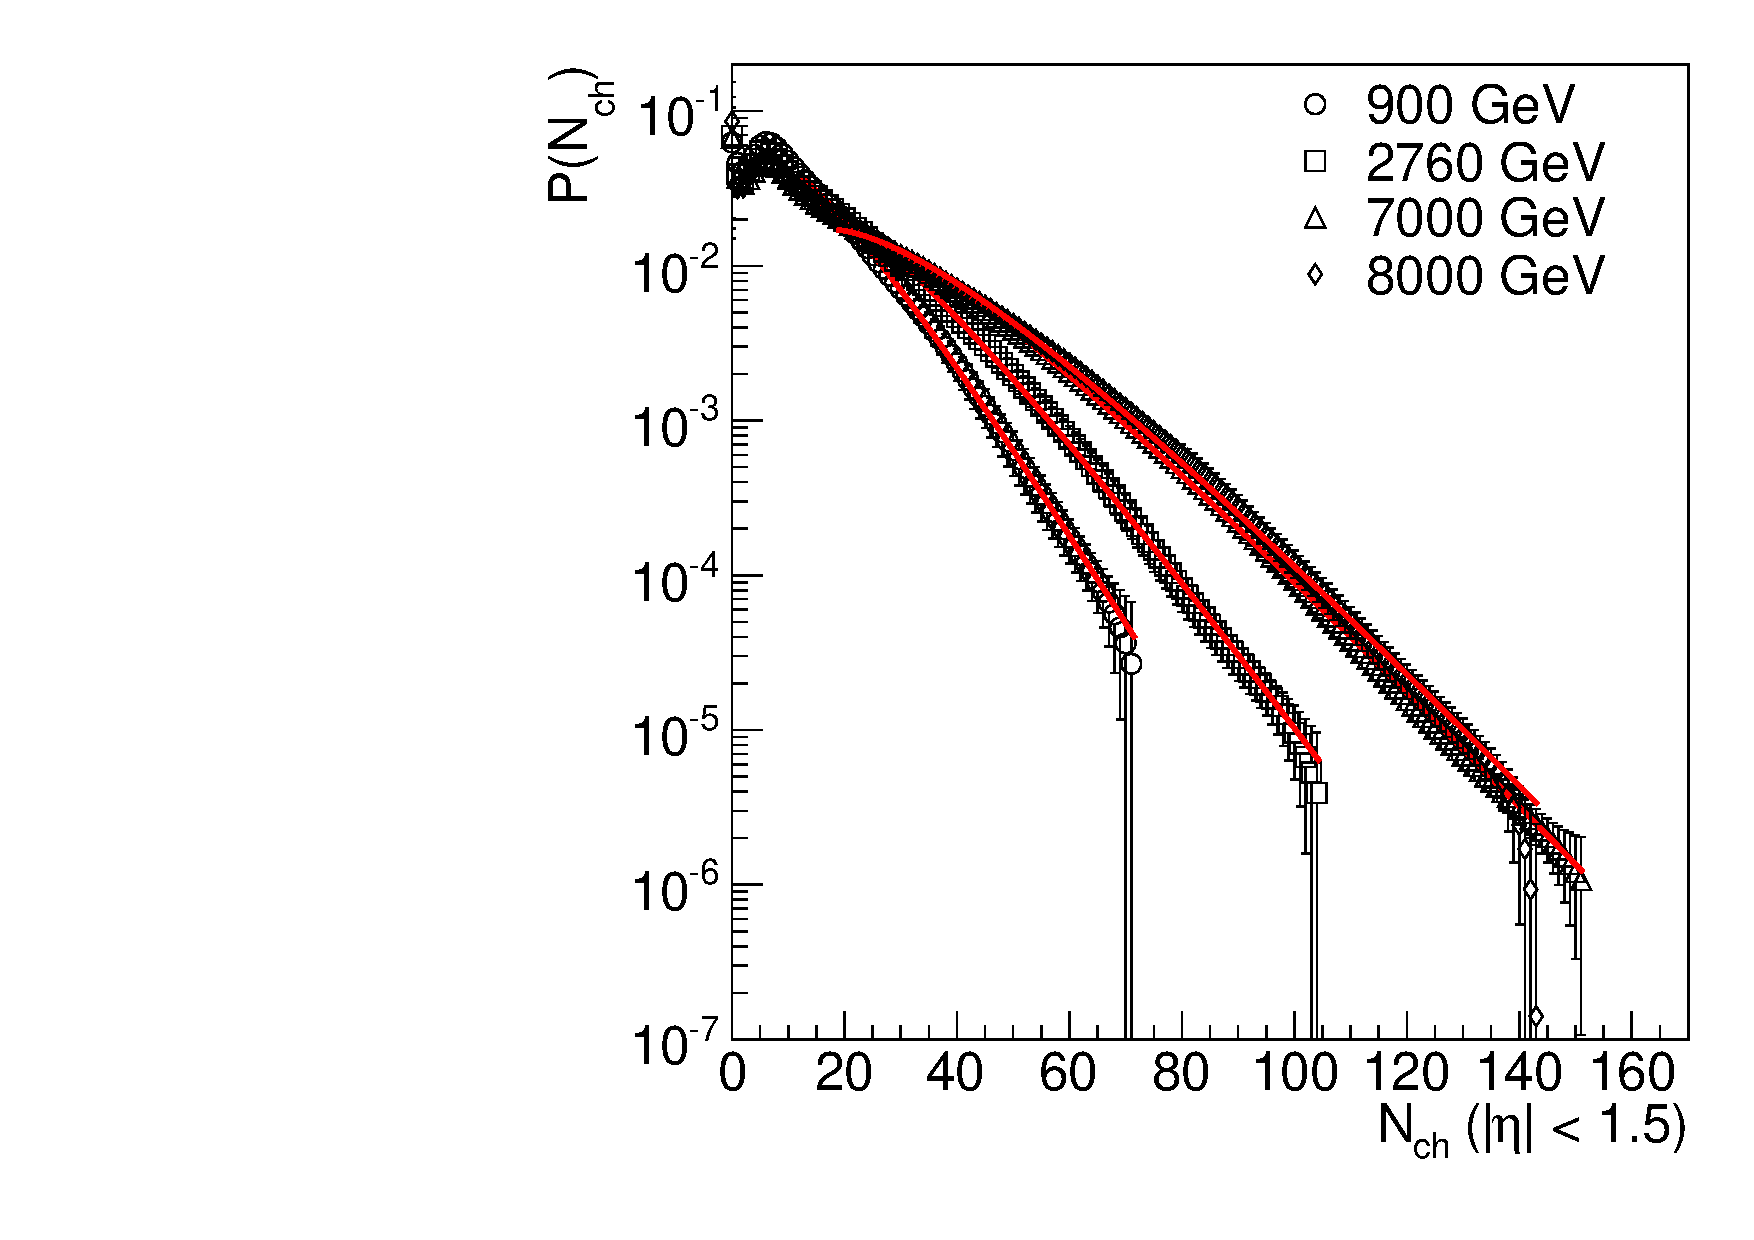
\includegraphics[width=0.49\linewidth]{\main/smallsystems/img/mult_data_1.pdf}
\hfill
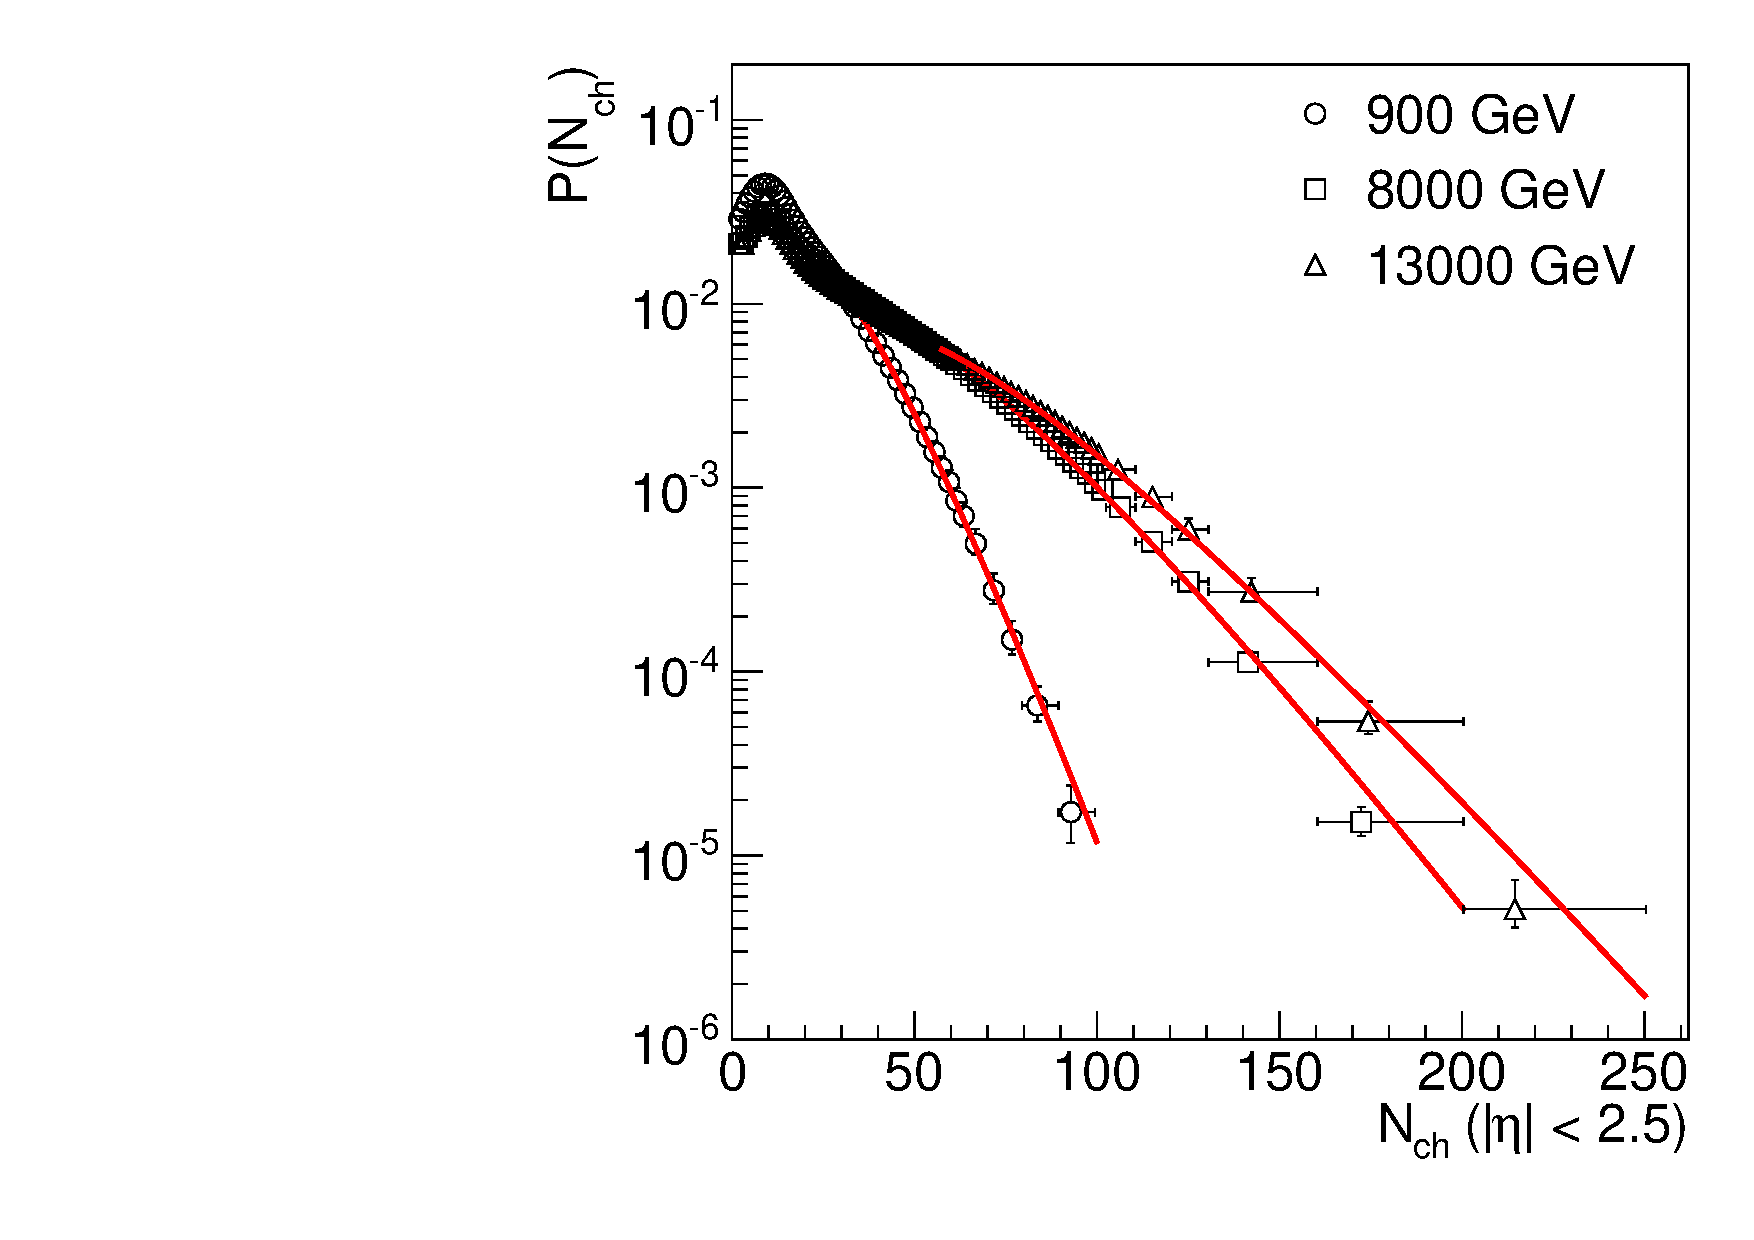
\includegraphics[width=0.49\linewidth]{\main/smallsystems/img/mult_data_11.pdf}
\caption{Multiplicity distributions measured by ALICE~\cite{Adam:2015gka} (left panel) and ATLAS~\cite{Aad:2010ac,Aad:2016xww} (right panel) overlaid by the fit with a negative binomial distribution. For details see text.}
\label{fig:smallsystems_mult_data}
\end{figure}

\begin{figure}[t]
\centering
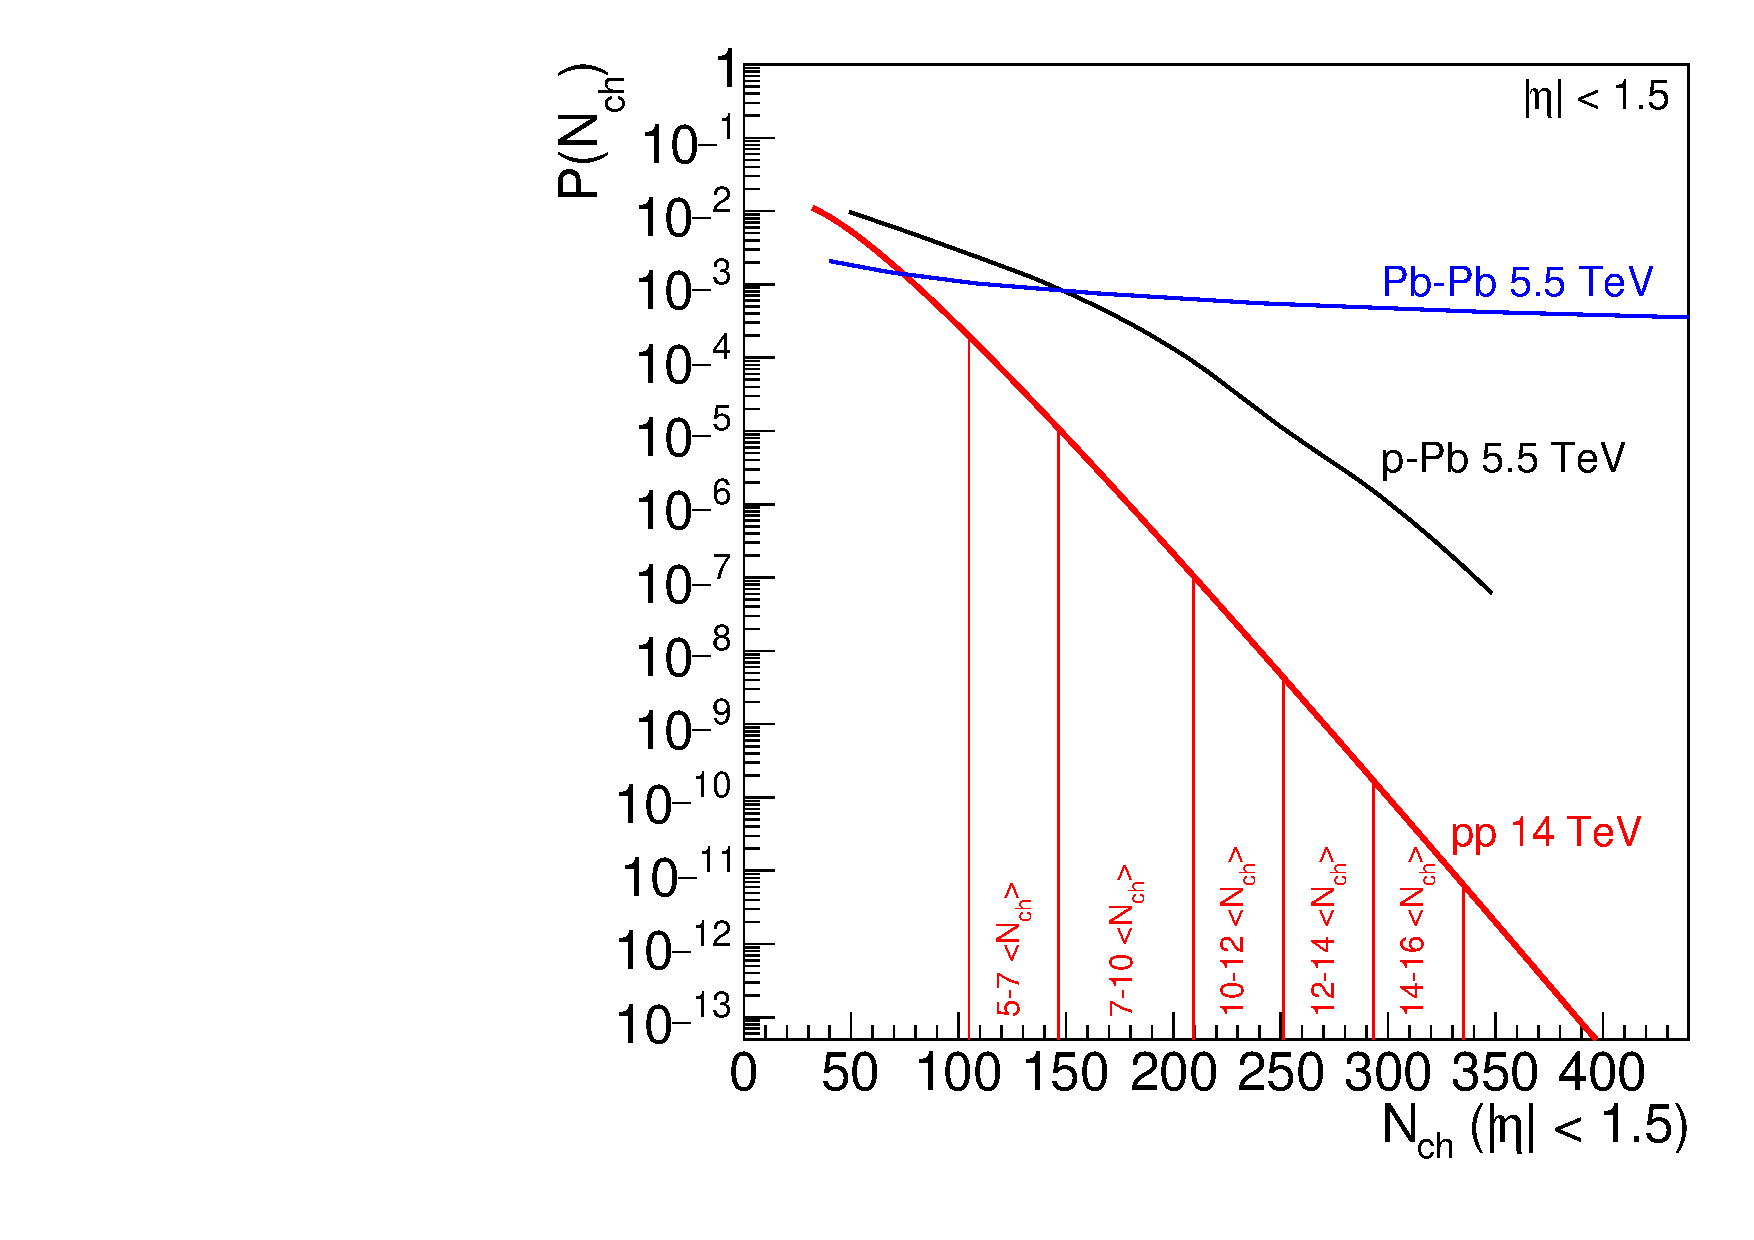
\includegraphics[width=0.32\linewidth]{\main/smallsystems/img/mult_extrapolation_alice.pdf}
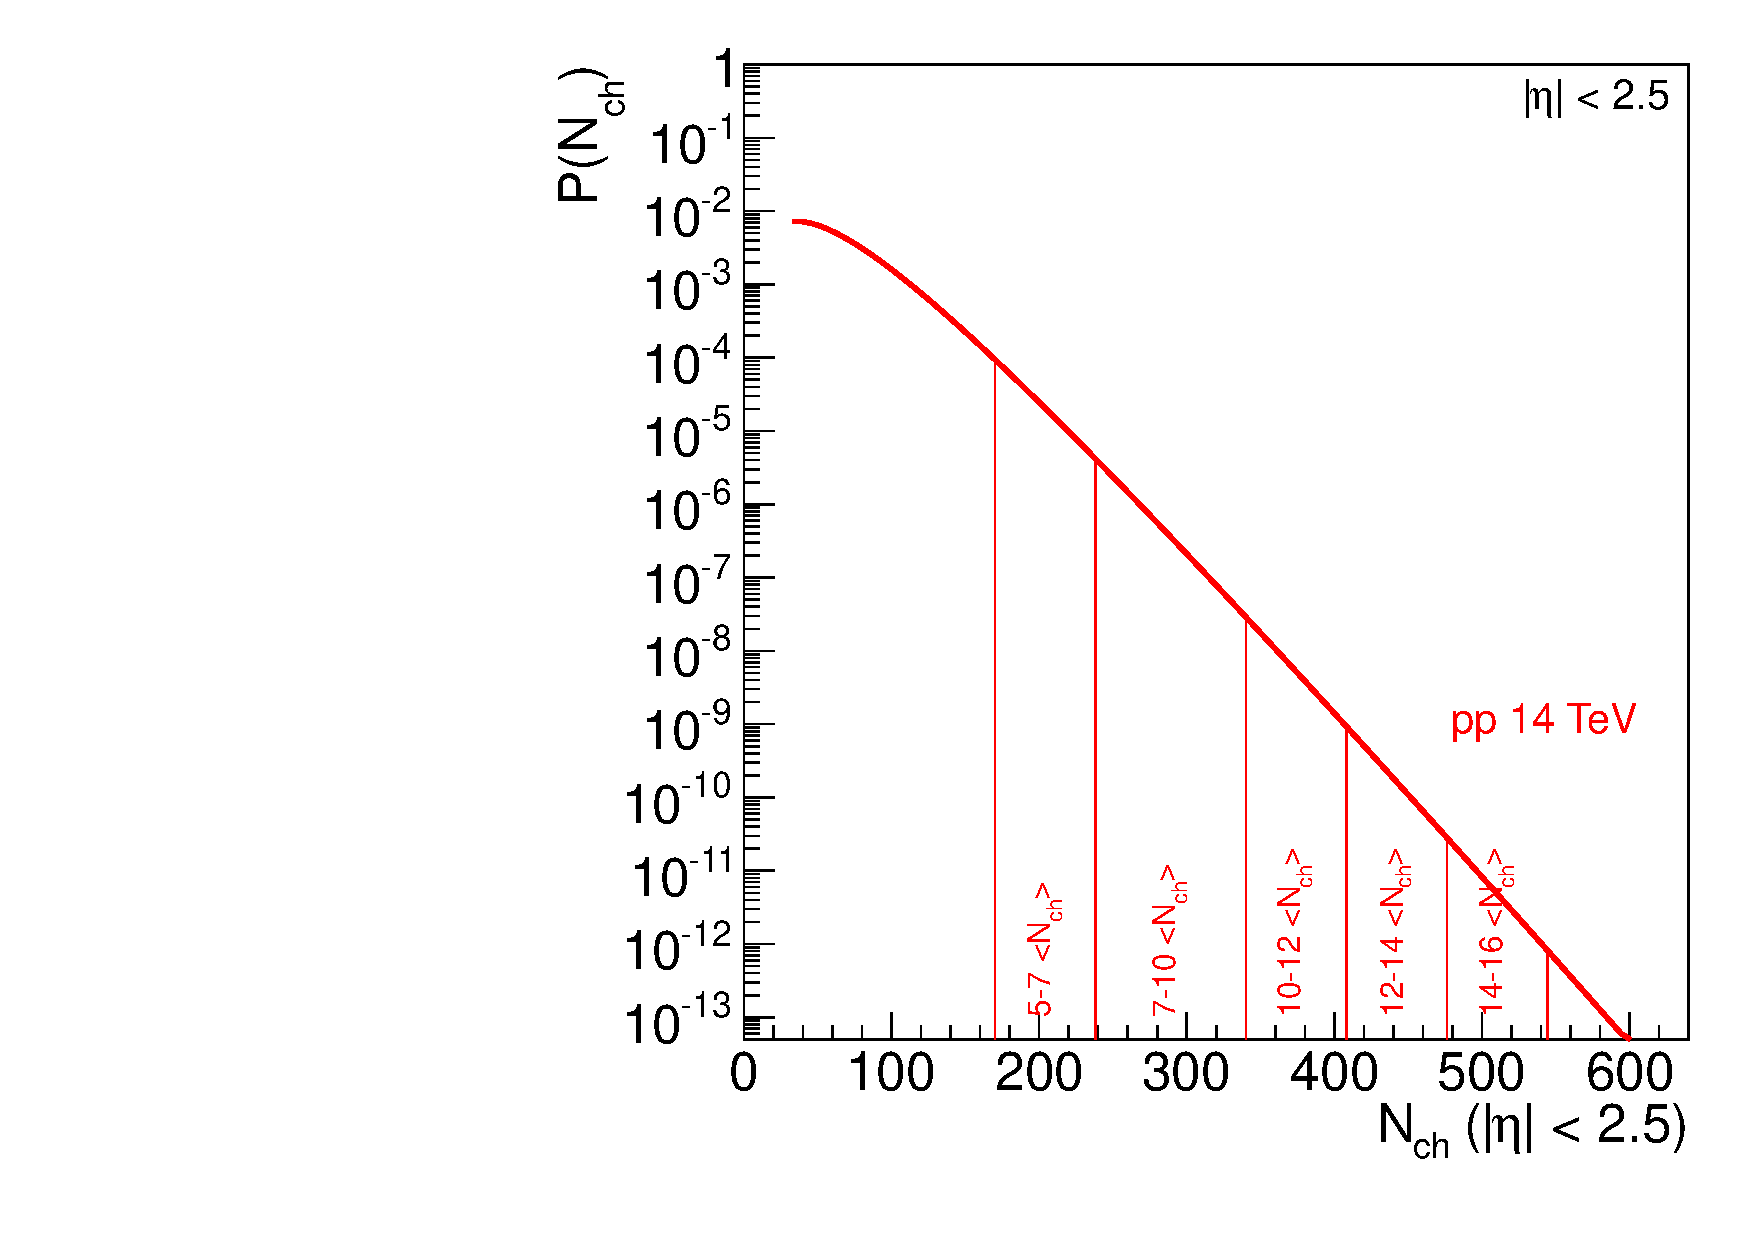
\includegraphics[width=0.32\linewidth]{\main/smallsystems/img/mult_extrapolation_atlas.pdf}
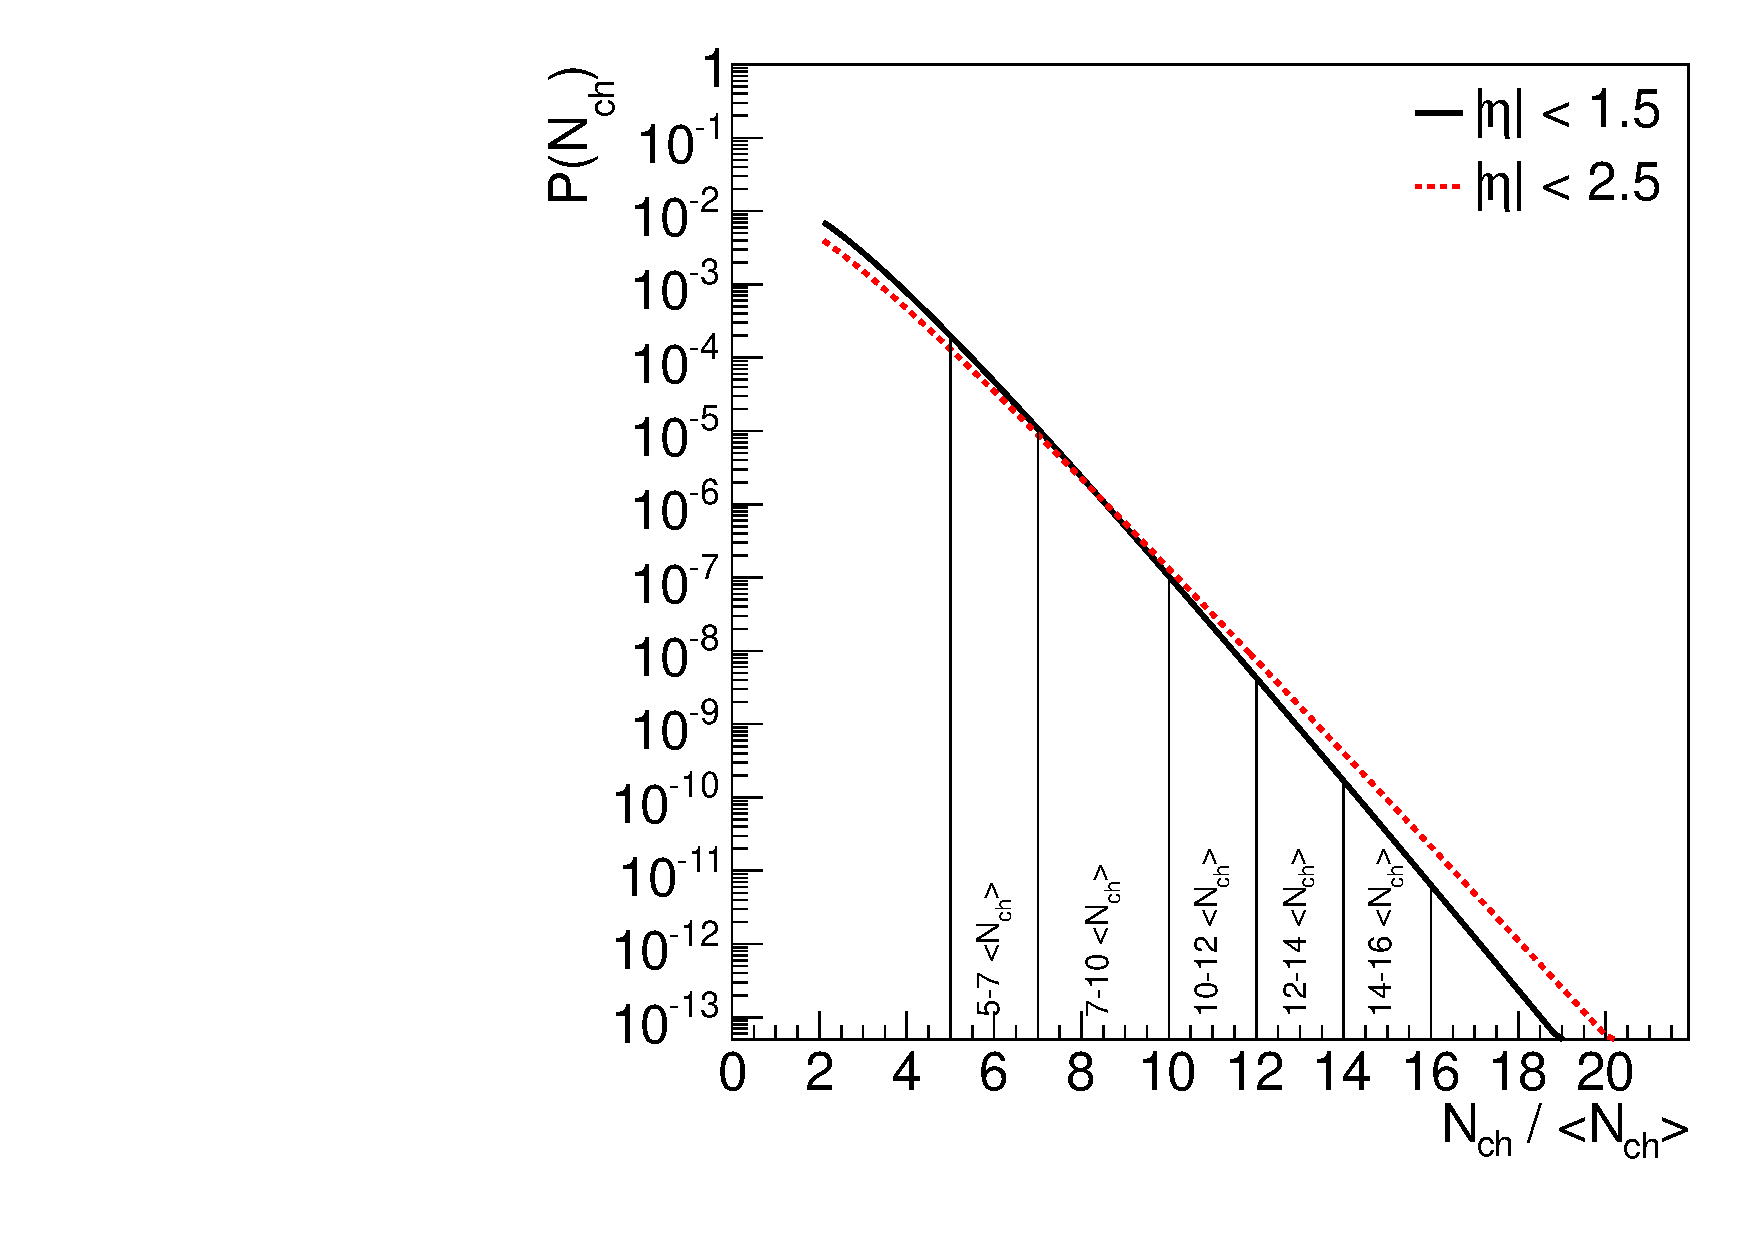
\includegraphics[width=0.32\linewidth]{\main/smallsystems/img/mult_extrapolation_comparison.pdf}
\caption{Extrapolated multiplicity distributions in pp collisions within $|\eta| < 1.5$ (left panel) and $|\eta| < 2.5$ (center panel). The indicated regions are (from left to right) 5--7, 7--10, 10--12, 12--14, 14--16 times the average multiplicity. In the left panel the multiplicity distribution of \PbPb and \pPb collisions is also plotted. The right panel compares these two distributions scaled by the average multiplicity. The extrapolation for $|\eta| < 2.5$ turns out to be a bit wider at large multiplicities; therefore the one based on $|\eta| < 1.5$ is used as baseline.}
\label{fig:smallsystems_mult_extrapolation}
\end{figure}

The resulting extrapolated multiplicity distribution for \unit[14]{\UTeV} is shown in Fig.~\ref{fig:smallsystems_mult_extrapolation} for the ALICE and ATLAS case. In addition, these are compared scaled by their respective average multiplicities. The agreement is rather good, with some discrepancy in the tail of the distribution. The extrapolation based on the smaller phase space region falls off more quickly with multiplicity, and is therefore used as the more conservative estimate for the extrapolations in this chapter.

\begin{figure}[t]
\centering
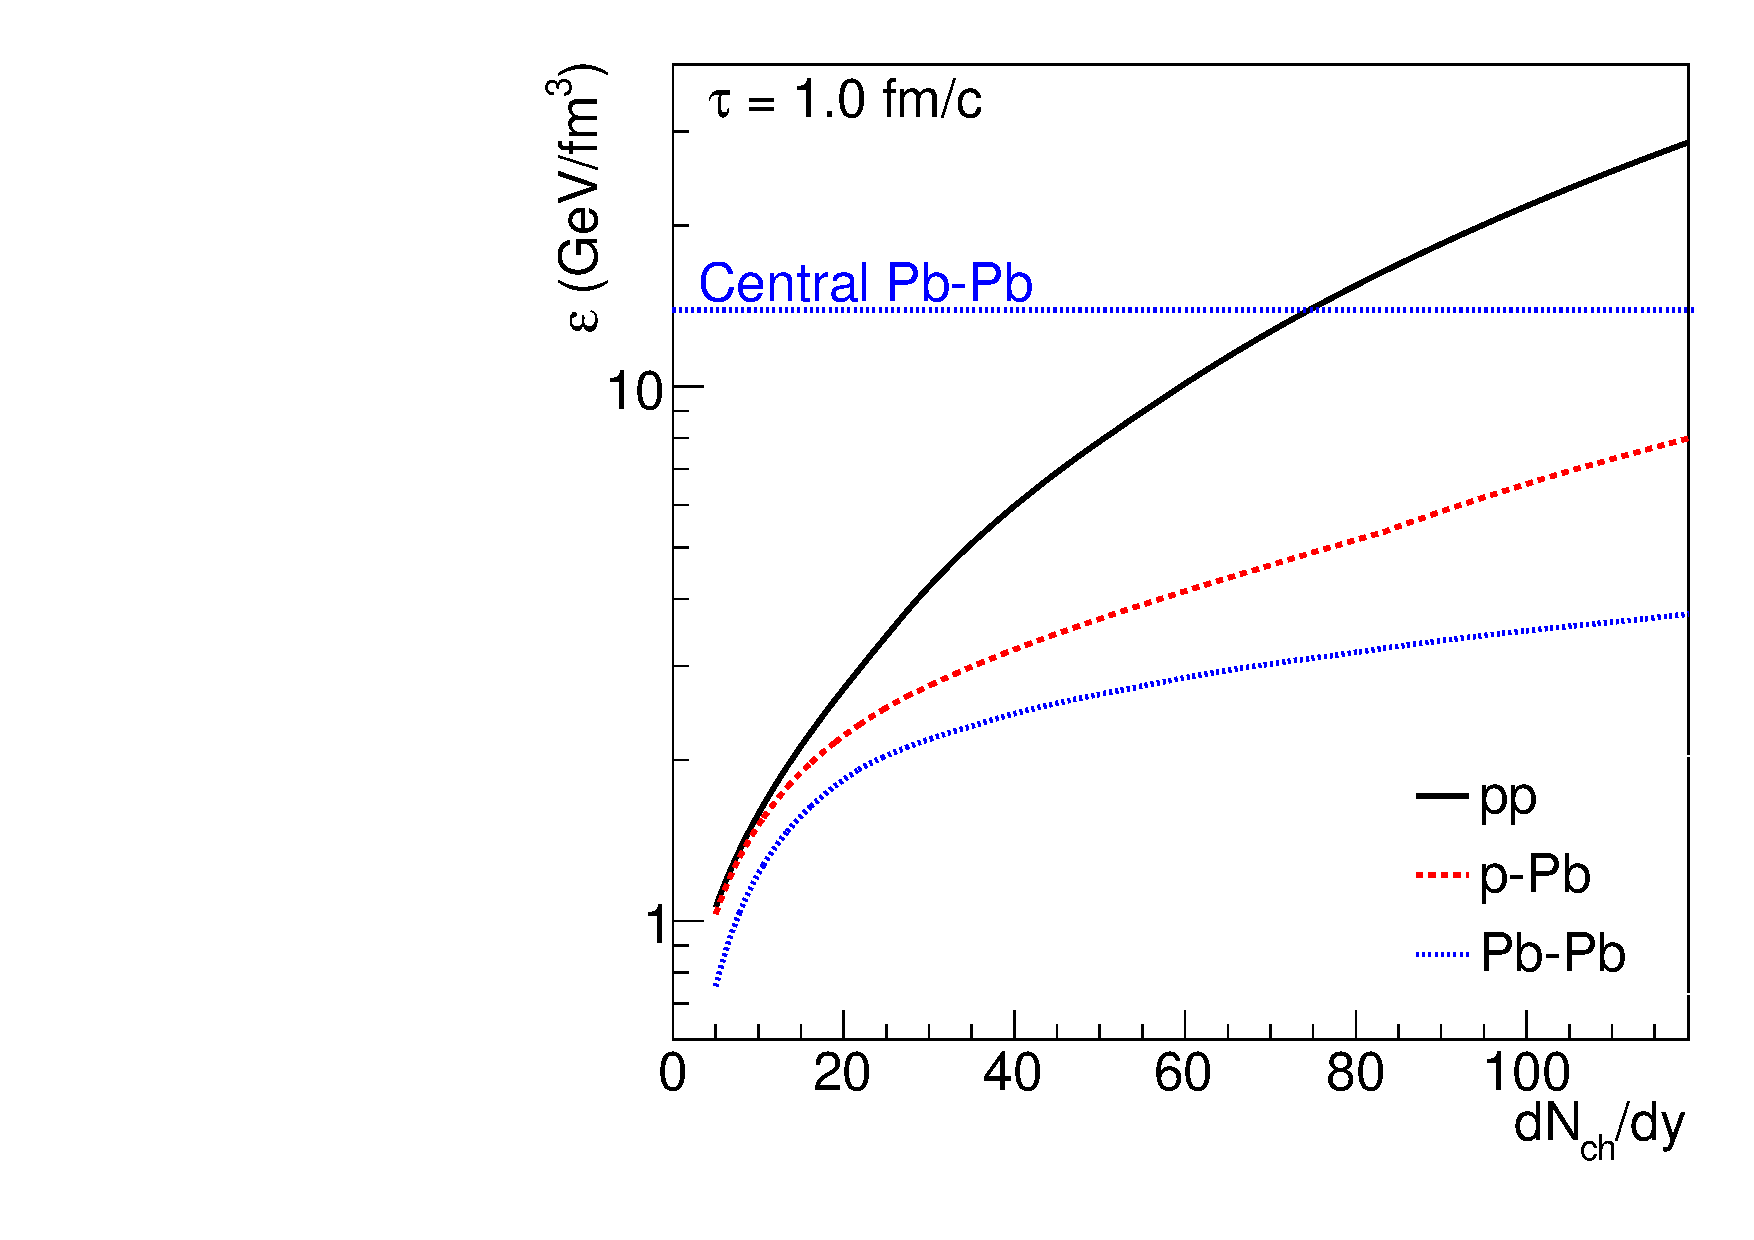
\includegraphics[width=0.5\linewidth]{\main/smallsystems/img/energy_density.pdf}
\caption{Energy density as a function of $\dNdy$ calculated by IP Glasma (solid lines) and with MC Glauber and the Bjorken formula (dashed lines); for details see text. Compared are \pp, \pPb and \PbPb collisions at $\tau = \unit[0.2]{fm/c}$. The horizontal line indicates the energy density reached in central \PbPb collisions ($\dNdy \approx 2000$).}
\label{fig:small_systems_energy_density}
\end{figure}

\subsubsection{Energy density}
While the multiplicity is a convenient and well defined observable to compare different collision systems, the underlying dynamics may be driven by other properties. In large collision systems, the energy density $\epsilon$ is often used to characterize the system and the expected effects. Figure~\ref{fig:small_systems_energy_density} shows an estimate of the energy density for \pp, \pPb and \PbPb collisions based on IP-Glasma~\cite{Bzdak:2013zma} as well as on the Bjorken estimate:
\begin{equation}
  \epsilon = \frac{1}{A \tau} \langle E \rangle \frac{3}{2} \frac{dN_{ch}}{dy}.
\end{equation}
For the latter, the input is the multiplicity-dependent $\meanpT$~\cite{Abelev:2013bla,Acharya:2018njl} as well as the multiplicity-dependent transverse overlap from a Glauber MC~\cite{Loizides:2017ack}. The energy density is calculated at fixed $\tau = \unit[0.2]{fm/c}$. It should be noted that these assumptions can be challenged and other ways to calculate $\epsilon$ are available. Here the aim is only to show that the energy density depends on the system at a fixed multiplicity, and can reach large values in \pp and \pPb collisions, of the order of central \PbPb collisions.

\subsubsection{Data-taking conditions and integrated luminosity for \pp collisions}
For the performance studies in this chapter, a high-multiplicity sample of $\Lint = \unit[200]{pb^{-1}}$ is assumed per experiment. In order to assure a clean trigger, collisions at low $\mu \approx 1$ are needed which requires special runs or special conditions at the end of fill for ATLAS, CMS and LHCb. ALICE generally runs at low $\mu$ and can collect a similar sample over a longer data-taking period.

Table~\ref{tab:smallsystems_pp} gives the fraction of cross-section and the number of events in five multiplicity classes:  5--7, 7--10, 10--12, 12--14 and 14--16 times the average multiplicity. Table~\ref{tab:smallsystems_pbpb} gives the number of events of bins with equivalent multiplicity than commonly measured multiplicity bins in \pPb and \PbPb collisions. For the calculation of the number of events $\sigma_{\rm inel} = \unit[78.4]{mb}$~\cite{Loizides:2017ack} is used. These tables are the key input for the performance figures presented in this chapter. 
The conversion of the provided $\dNdeta$ to multiplicity ranges with larger pseudorapidity coverage is done for simplicity assuming a flat pseudorapidity distribution within $|\eta| < 2.5$. For the conversion to a phase space with a lower $\pT$ cut as employed in many current measurements a set of conversation factors is used, listed in Tab.~\ref{tab:smallsystems_conversion}.

\begin{table}
\centering
\begin{tabular}{c|c|c|c|c}
Range & $\dNdeta$ & Fraction & Events per pb$^{-1}$ & Events in \unit[200]{pb$^{-1}$} \\
\hline
5--7 \meannch     & 35--49   & 2.4e-03       & 1.9e+08       & 3.7e+10 \\
7--10 \meannch    & 49--70   & 1.3e-04       & 1.0e+07       & 2.0e+09 \\
10--12 \meannch   & 70--84   & 1.1e-06       & 9.0e+04       & 1.8e+07 \\
12--14 \meannch   & 84--98   & 4.7e-08       & 3.7e+03       & 7.3e+05 \\
14--16 \meannch   & 98--112  & 1.8e-09       & 1.4e+02       & 2.8e+04 \\
\hline
\end{tabular}
\caption{Number of pp events at \unit[14]{\UTeV} in selected high-multiplicity bins.}
\label{tab:smallsystems_pp}
\end{table}

\begin{table}
\centering
\begin{tabular}{l|c|c|c}
Range & $\dNdeta$ & Events per pb$^{-1}$ & Events in \unit[200]{pb$^{-1}$} \\
\hline
0--5\% \pPb   & 41--56        & 4.9e+07       & 9.8e+09 \\
5--10\% \pPb  & 34--41        & 1.9e+08       & 3.8e+10 \\
10--20\% \pPb & 27--34        & 6.6e+08       & 1.3e+11 \\
\hline
60--65\% \PbPb    & 98--137       & 1.5e+02       & 3.0e+04 \\
65--70\% \PbPb    & 68--98        & 1.6e+05       & 3.1e+07 \\
70--75\% \PbPb    & 45--68        & 2.1e+07       & 4.2e+09 \\
75--80\% \PbPb    & 29--45        & 5.9e+08       & 1.2e+11 \\
\hline
\end{tabular}
\caption{Number of events in pp collisions at \unit[14]{\UTeV} sliced in equivalent multiplicity bins as in \pPb and \PbPb collisions.}
\label{tab:smallsystems_pbpb}
\end{table}

\begin{table}
\centering
\begin{tabular}{c|c|c|c|c|c}
\backslashbox{$|\eta|$}{$\pT$} & $> \unit[0.1]{\UGeVc}$ & $> \unit[0.2]{\UGeVc}$ & $> \unit[0.3]{\UGeVc}$ & $> \unit[0.4]{\UGeVc}$ & $> \unit[0.5]{\UGeVc}$ \\
\hline
$|\eta| < 1.5$ & 1.03 & 1.11 & 1.22 & 1.31 & 1.40 \\
\hline
$|\eta| < 2.4$ & 1.04 & 1.14 & 1.27 & 1.42 & 1.55 \\
\hline
\end{tabular}
\caption{Conversion factors between $\nch$ with a \pT threshold, and $\nch$ including particles down to $\pT = 0$. The factor shown is $\nch / \nch(\pT > X)$, extracted with Pythia 8, tune CUETP8M1~\cite{Khachatryan:2015pea}. A potential multiplicity dependence of this factor is neglected for the projections in this chapter.}
\label{tab:smallsystems_conversion}
\end{table}

\subsection{Global-event properties}
\label{sect:smallsystems_global}
  
The measurement of global-event observables in rare high-multiplicity \pp collisions are of interest in itself. The shape of the multiplicity distribution, which has been largely extrapolated in the previous section, is today a challenge for models. It is not clear which mechanisms produce very large multiplicity events and therefore the shape of the distribution is an important input. 
Furthermore, studies of $\meanpT$ as a function of multiplicity~\cite{Abelev:2013bla} have shown a strong increase with multiplicity. However, those measurements exist only up to $\dNdeta \approx 55$, while the measurements at HL-LHC promise a measurement beyond twice that value. 

The shape of the multiplicity distribution and the growth of $\meanpT$ are closely connected to the physics of multiple parton interactions: high-multiplicity collisions are understood as originating from the collision of multiple partons within the same \pp collisions. It has been shown that the number of (low momentum transfer) parton interactions increases linearly with multiplicity with a possible saturation at large multiplicity~\cite{Abelev:2013sqa}. The prospect of showing that there is a maximal number of parton interactions is an important ingredient to a revised conceptual understanding of particle production in high-energy \pp collisions. Together with the studies of symmetric cumulants (see the subsequent Section), HL-LHC will determine not only if all partons can be involved in a collision but also their structure within the proton.

\subsection{Particle correlations}
\label{sect:smallsystems_correlations}

\begin{figure}[t]
\centering
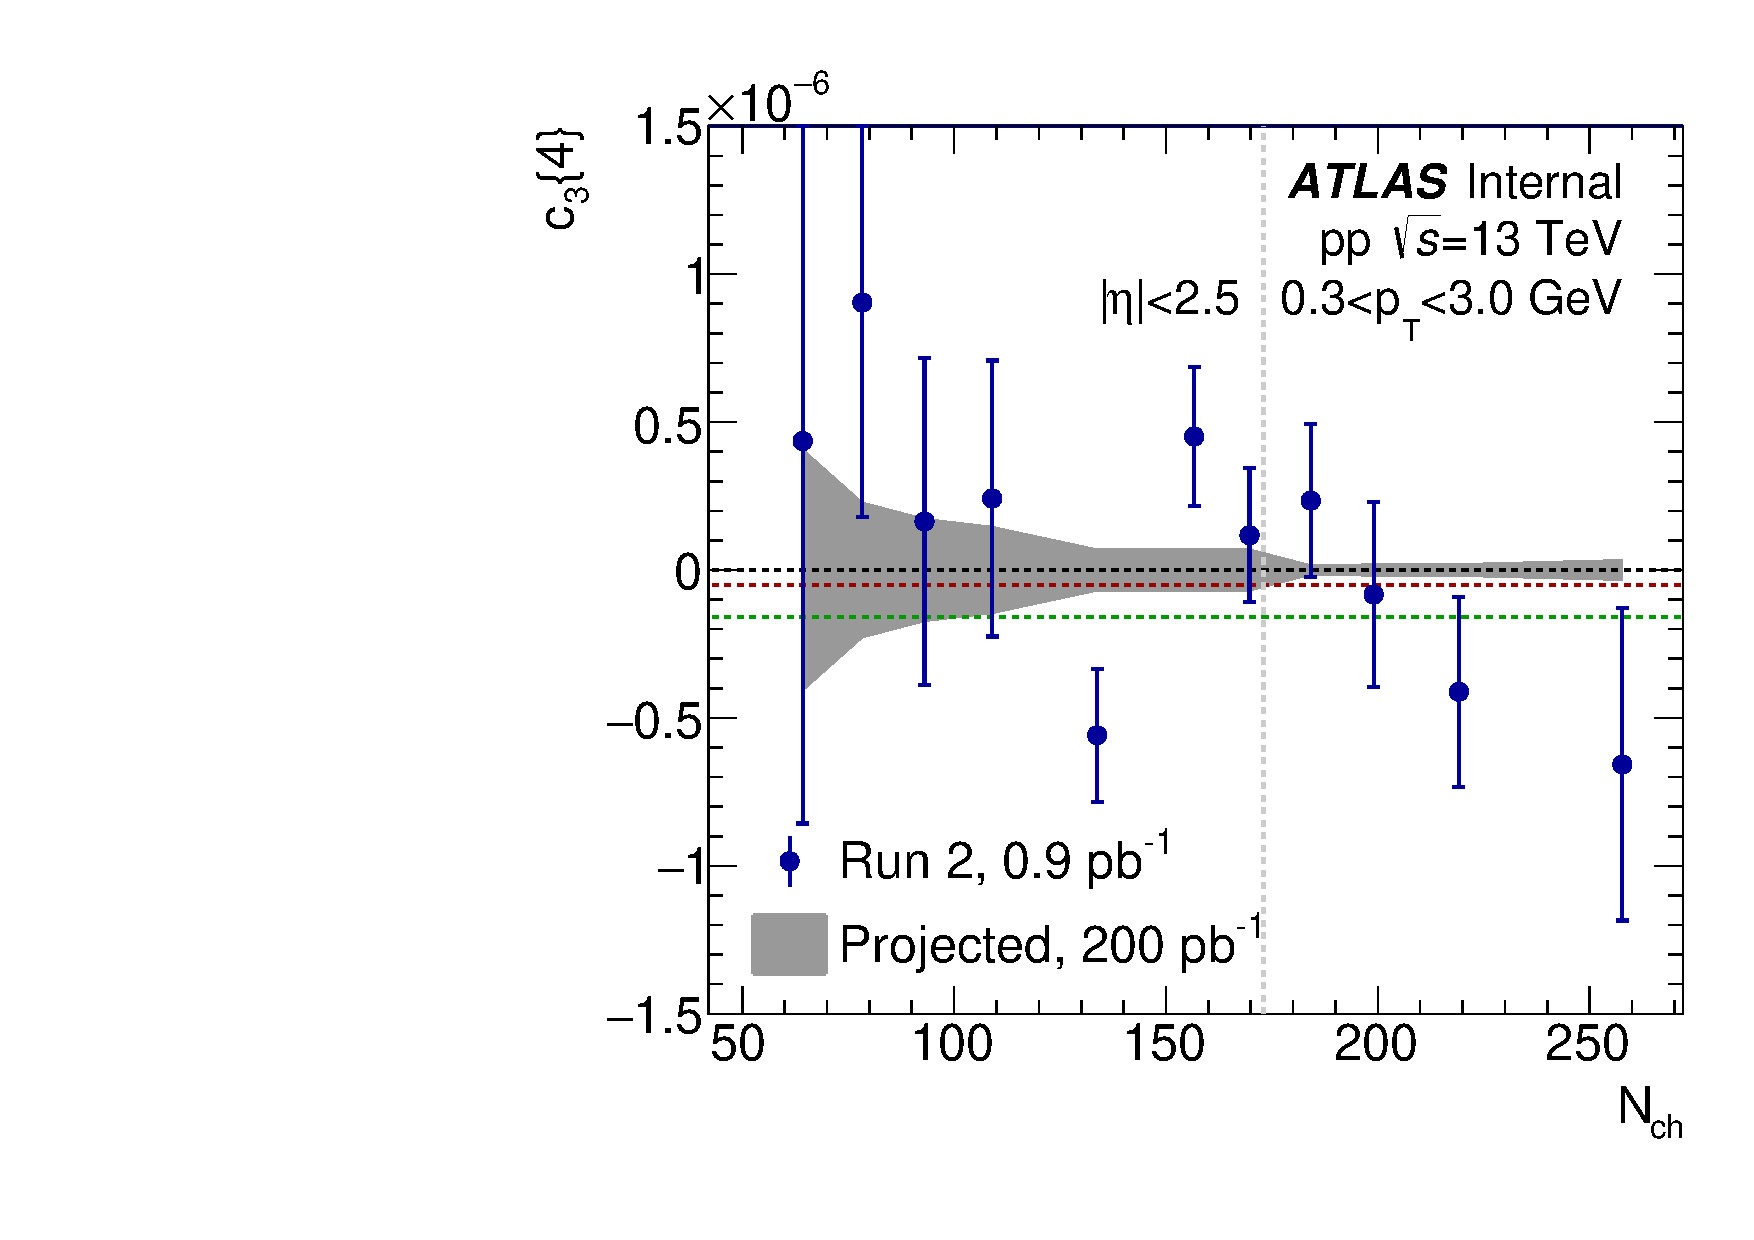
\includegraphics[width=.49\linewidth]{\main/smallsystems/img/c_3_4_pp.pdf}
\hfill
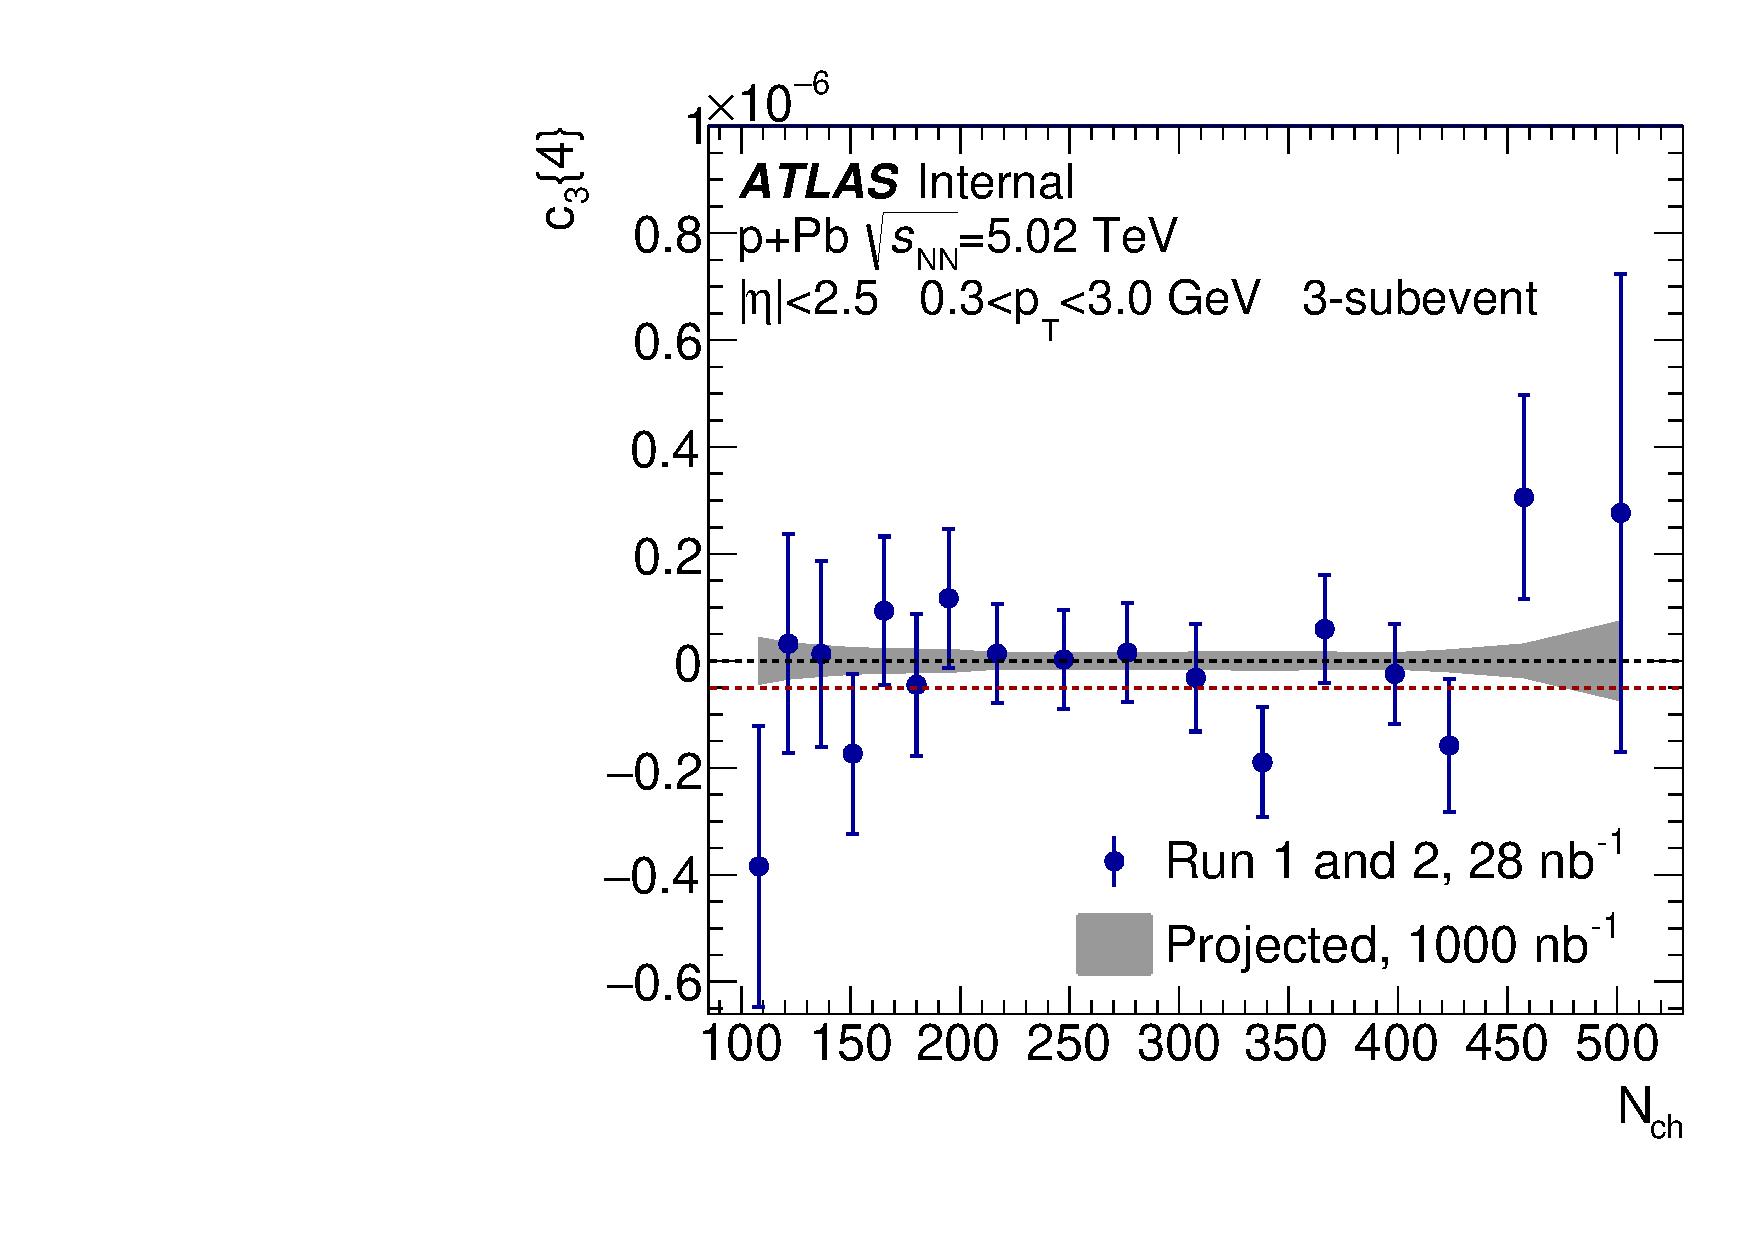
\includegraphics[width=.49\linewidth]{\main/smallsystems/img/c_3_4_pPb.pdf}
\caption{4-particle cumulants $c_3\{4\}$ measured with 3-subevent method for \pp (left panel) and \pPb collisions (right panel) as a function of $\nch$ ($|\eta| < 2.5$ and $0.3 < \pT < \unit[3]{\UGeVc}$). Only statistical uncertainties are shown in the figure and the gray band represents the projected statistical uncertainty, with $c_3\{4\}$ assumed to be zero. The red and green dash lines represent $1.5\%$ and $2.0\%$ $v_3\{4\}$ signal, respectively. The vertical line in the left panel indicates the transition between minimum-bias and high-multiplicity triggered data. Figures from Ref.~\cite{ATL-PHYS-PUB-2018-020}.}
\label{fig:smallsystems_corr_cumulants}
\end{figure}

The measurements of two-particle correlations and higher-order cumulants have been the initial observations of collective-like effects in small systems. In \pp collisions, two distinct regions are of interest at HL-LHC: the high-multiplicity tail to compare to \pPb and \PbPb collisions and the low-multiplicity regions to investigate the onset of these effects. In the following, several performance estimates are given as examples for the rich physics which can be addressed.

State-of-the-art measured 4-particle cumulants of $\vthree$ ($c_3\{4\}$) in \pp and \pPb collisions are presented in Fig.~\ref{fig:smallsystems_corr_cumulants} overlaid with the projection for HL-LHC.
In order to remove non-flow contributions, the 3-subevent method is applied. In \pp collisions, with the data collected in Run 2, the statistical uncertainties are large and the $c_3\{4\}$ values are consistent with zero in most of the $\nch$ range. On the contrary, in large systems, significant non-zero $c_3\{4\}$ up to $-0.4 \cdot 10^{-6}$ depending on centrality has been measured~\cite{Aad:2014vba}, which reflects the nucleonic fluctuations in the initial state. Whether similar behaviour is observed in small systems still needs to be confirmed. The increase in luminosity in Run 3 and Run 4 provides a great opportunity to measure $c_3\{4\}$ in pp with high precision: the statistics are sufficient to measure a signal as small as $v_3\{4\} = 1.5\%$ for $\nch \gtrapprox 170$, while 2\% are accessible with large significance over a wide multiplicity range ($\nch \gtrapprox 100$). Similarly, in \pPb collision, the current result shows that $c_3\{4\}$ is consistent with zero, but increased statistics will help to detect a potential non-zero $c_3\{4\}$ smaller than $1.5\%$ for $100 \lessapprox \nch \lessapprox 500$. Similarly, the precision of the already measured non-zero $c_2\{4\}$ will be greatly improved~\cite{ATL-PHYS-PUB-2018-020}.

\begin{figure}[t!]
\centering
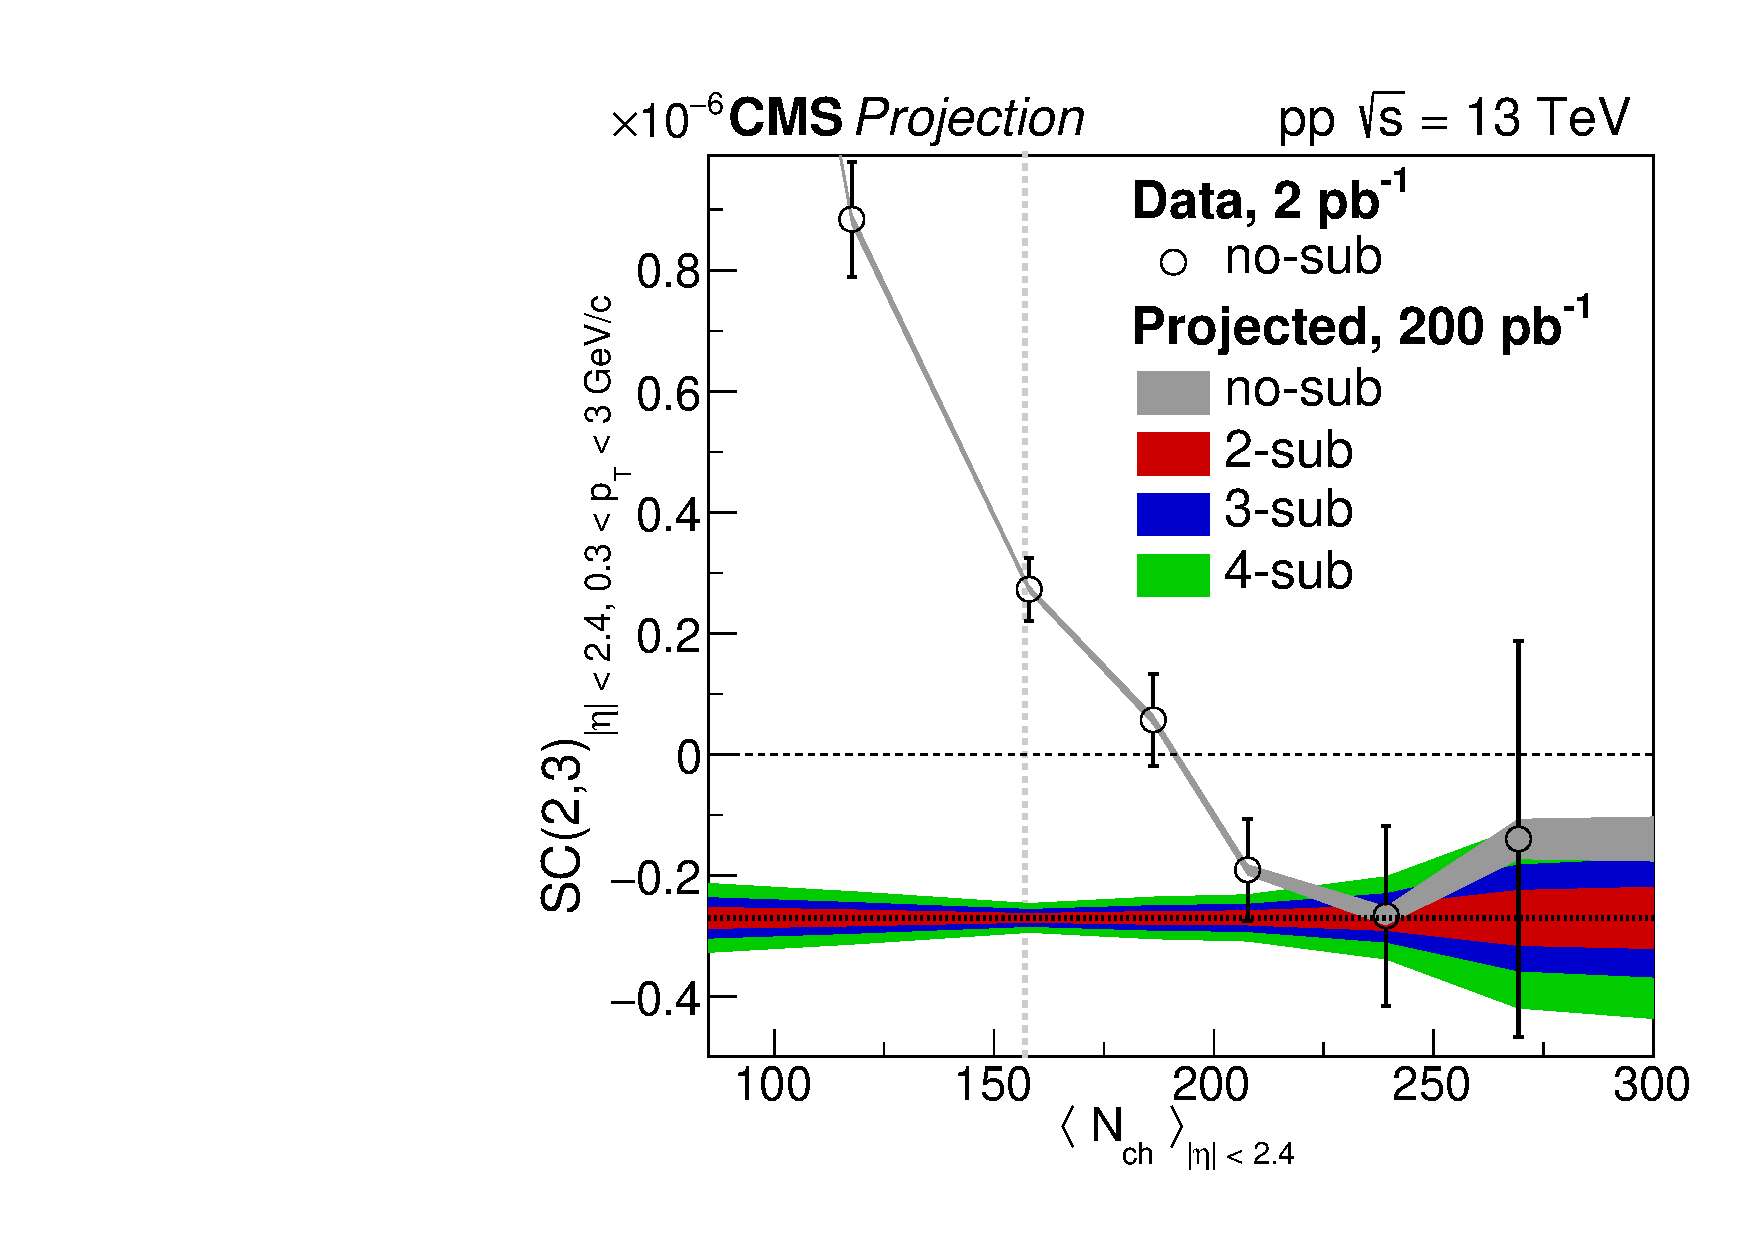
\includegraphics[width=0.48\linewidth]{\main/smallsystems/img/HLLHC_SC_pp13TeV.pdf}
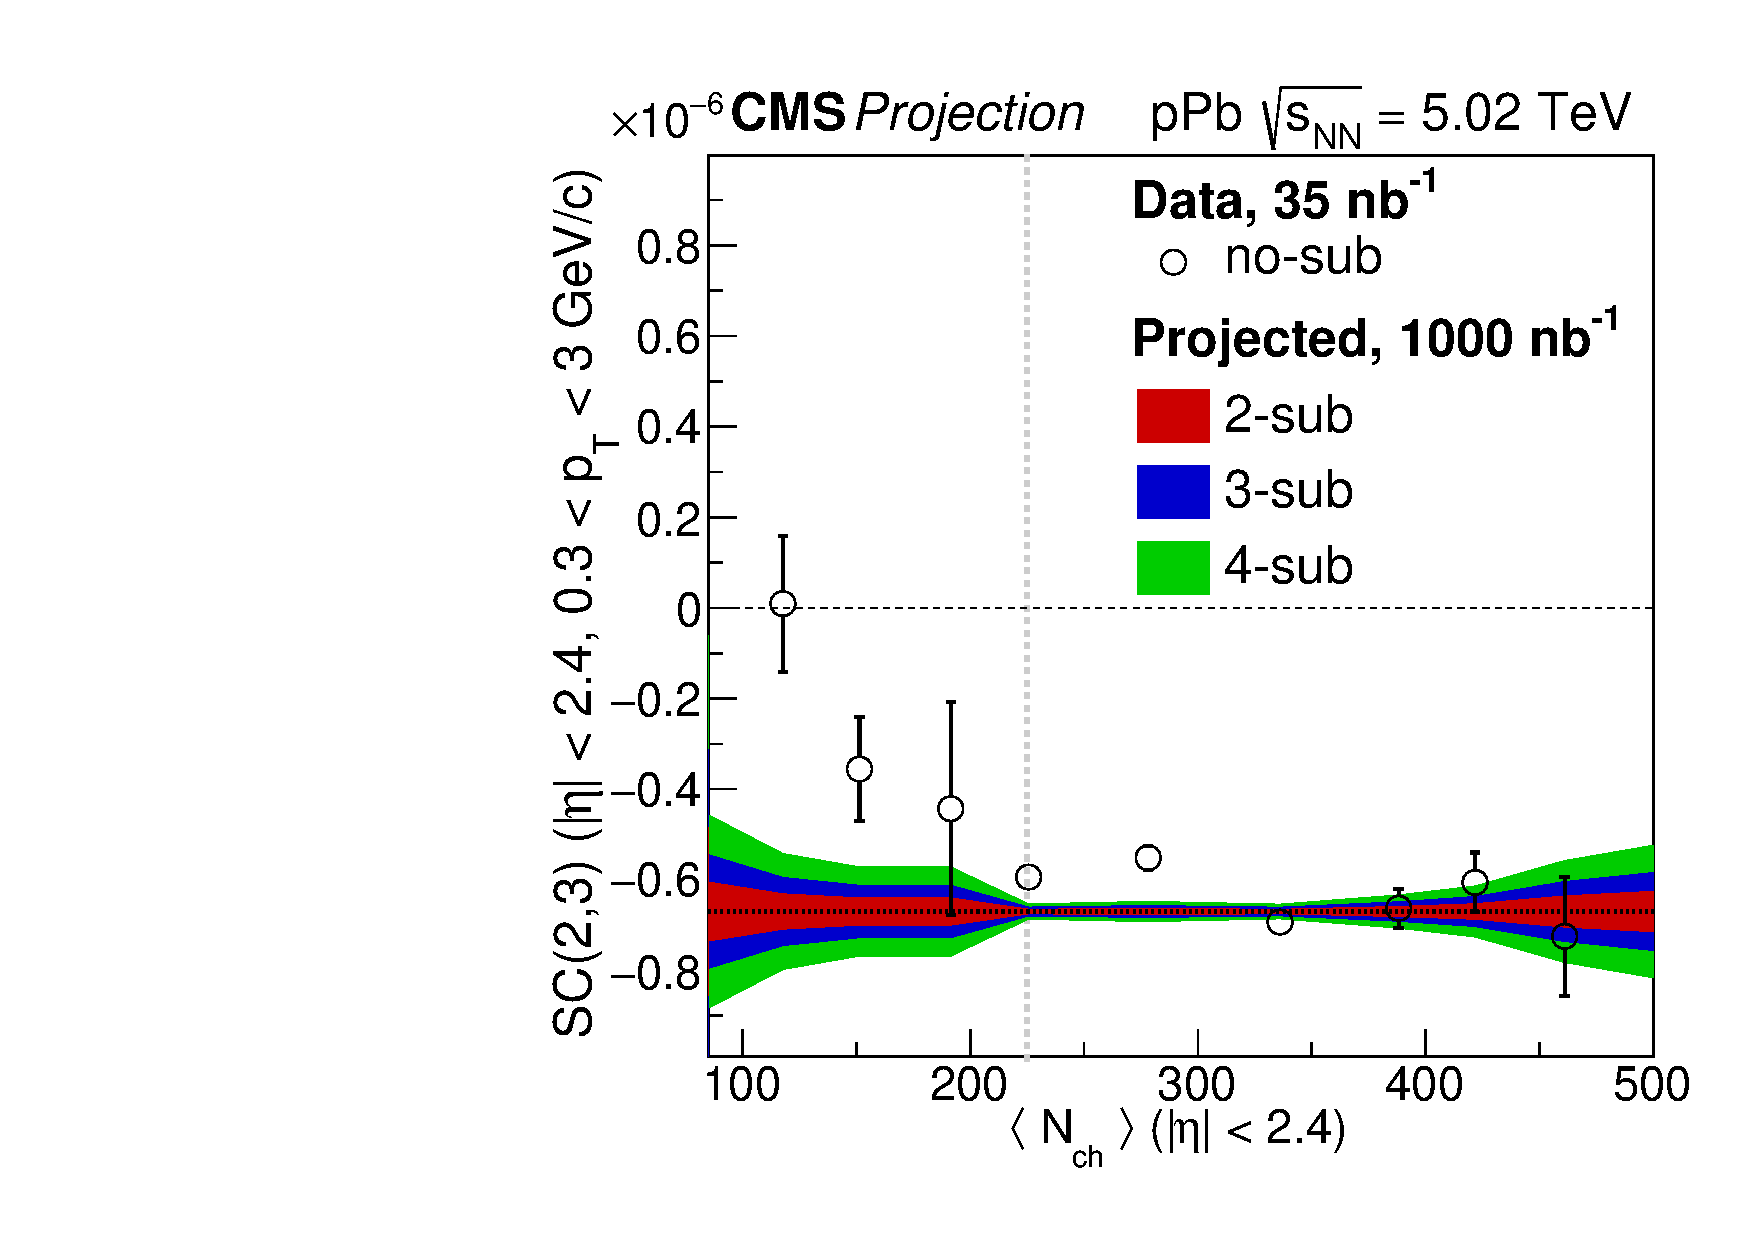
\includegraphics[width=0.48\linewidth]{\main/smallsystems/img/HLLHC_SC_pPb_5TeV.pdf}
\caption{Symmetric cumulants extracted with and without applying subevents for \pp (left panel) and \pPb collisions (right panel) as a function of $\nch$ ($|\eta| < 2.4$ and $0.3 < \pT < \unit[3]{\UGeVc}$). The projected reach is shown for the case of 2, 3 and 4 subevents assuming a constant signal as a function of multiplicity indicated by the lower horizontal line. The vertical line indicates the transition between minimum-bias and high-multiplicity triggered data. Figures from Ref.~\cite{CMS-PAS-FTR-18-026}. UNDER APPROVAL.}
\label{fig:smallsystems_corr_symmetriccumulants}
\end{figure}

\begin{figure}[t]
\centering
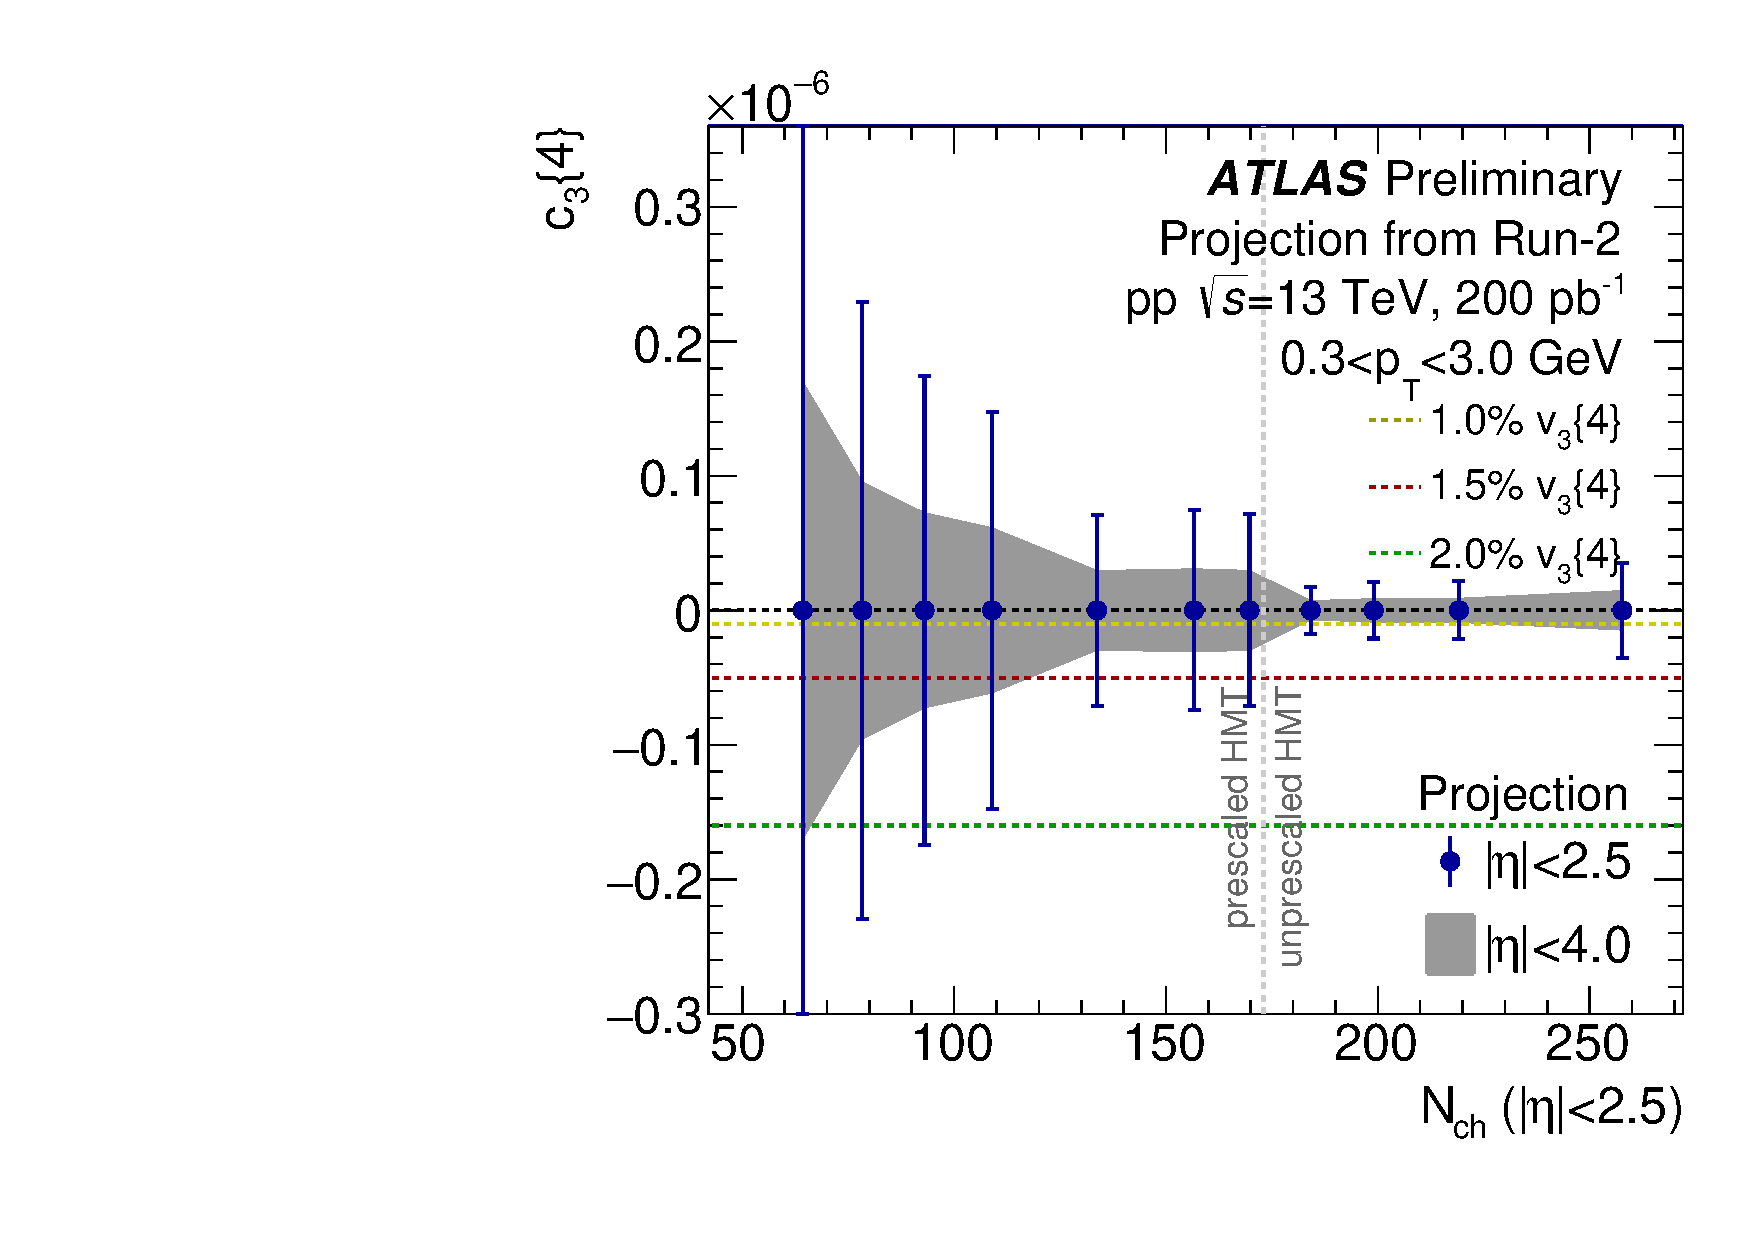
\includegraphics[width=.49\linewidth]{\main/smallsystems/img/c_3_4_pp_eta4.pdf}
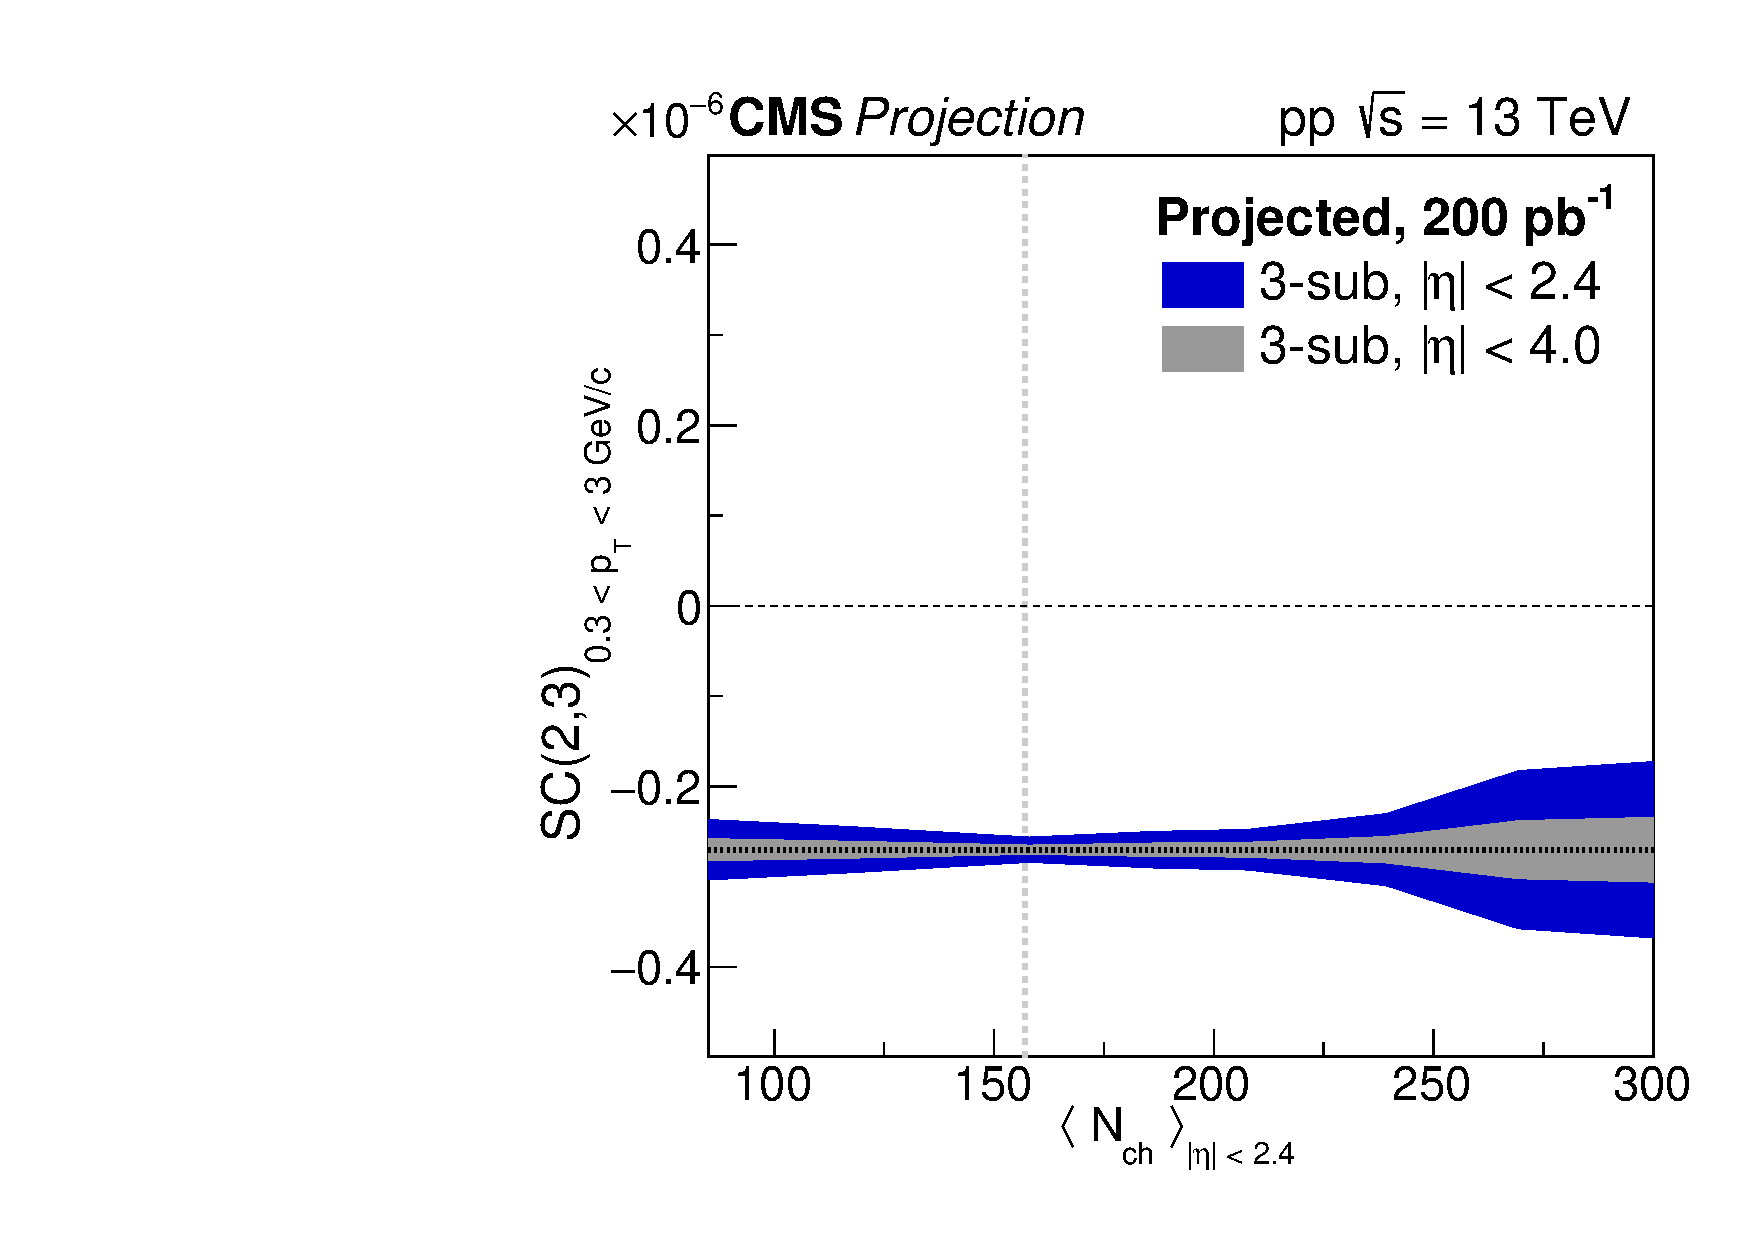
\includegraphics[width=.49\linewidth]{\main/smallsystems/img/HLLHC_SC_extcov13TeV.pdf}
\caption{Demonstration of the influence of the larger tracking acceptances for ATLAS and CMS available in Run 4. Left panel: 4-particle cumulant $c_3\{4\}$ (as in the left panel of Fig.~\ref{fig:smallsystems_corr_cumulants}) for \pp collisions with $\Lint = \unit[200]{pb^{-1}}$. The data points indicate the reach with the detector in Run 3 ($|\eta| < 2.5$) while the gray band the enlarged acceptance of $|\eta| < 4$ in Run 4. The yellow, red and green dash lines represent $1.0\%$, $1.5\%$ and $2.0\%$ $v_3\{4\}$ signal, respectively. Figure from Ref.~\cite{ATL-PHYS-PUB-2018-020}. Right panel: Symmetric cumulants with 3 subevents (as in left panel of Fig.~\ref{fig:smallsystems_corr_symmetriccumulants}) for \pp collisions with $\Lint = \unit[200]{pb^{-1}}$. Two blue (gray) area indicates the projected uncertainty for Run 3 (4). Figure from Ref.~\cite{}. UNDER APPROVAL.}
\label{fig:smallsystems_corr_eta4}
\end{figure}

\begin{figure}[t!]
\centering
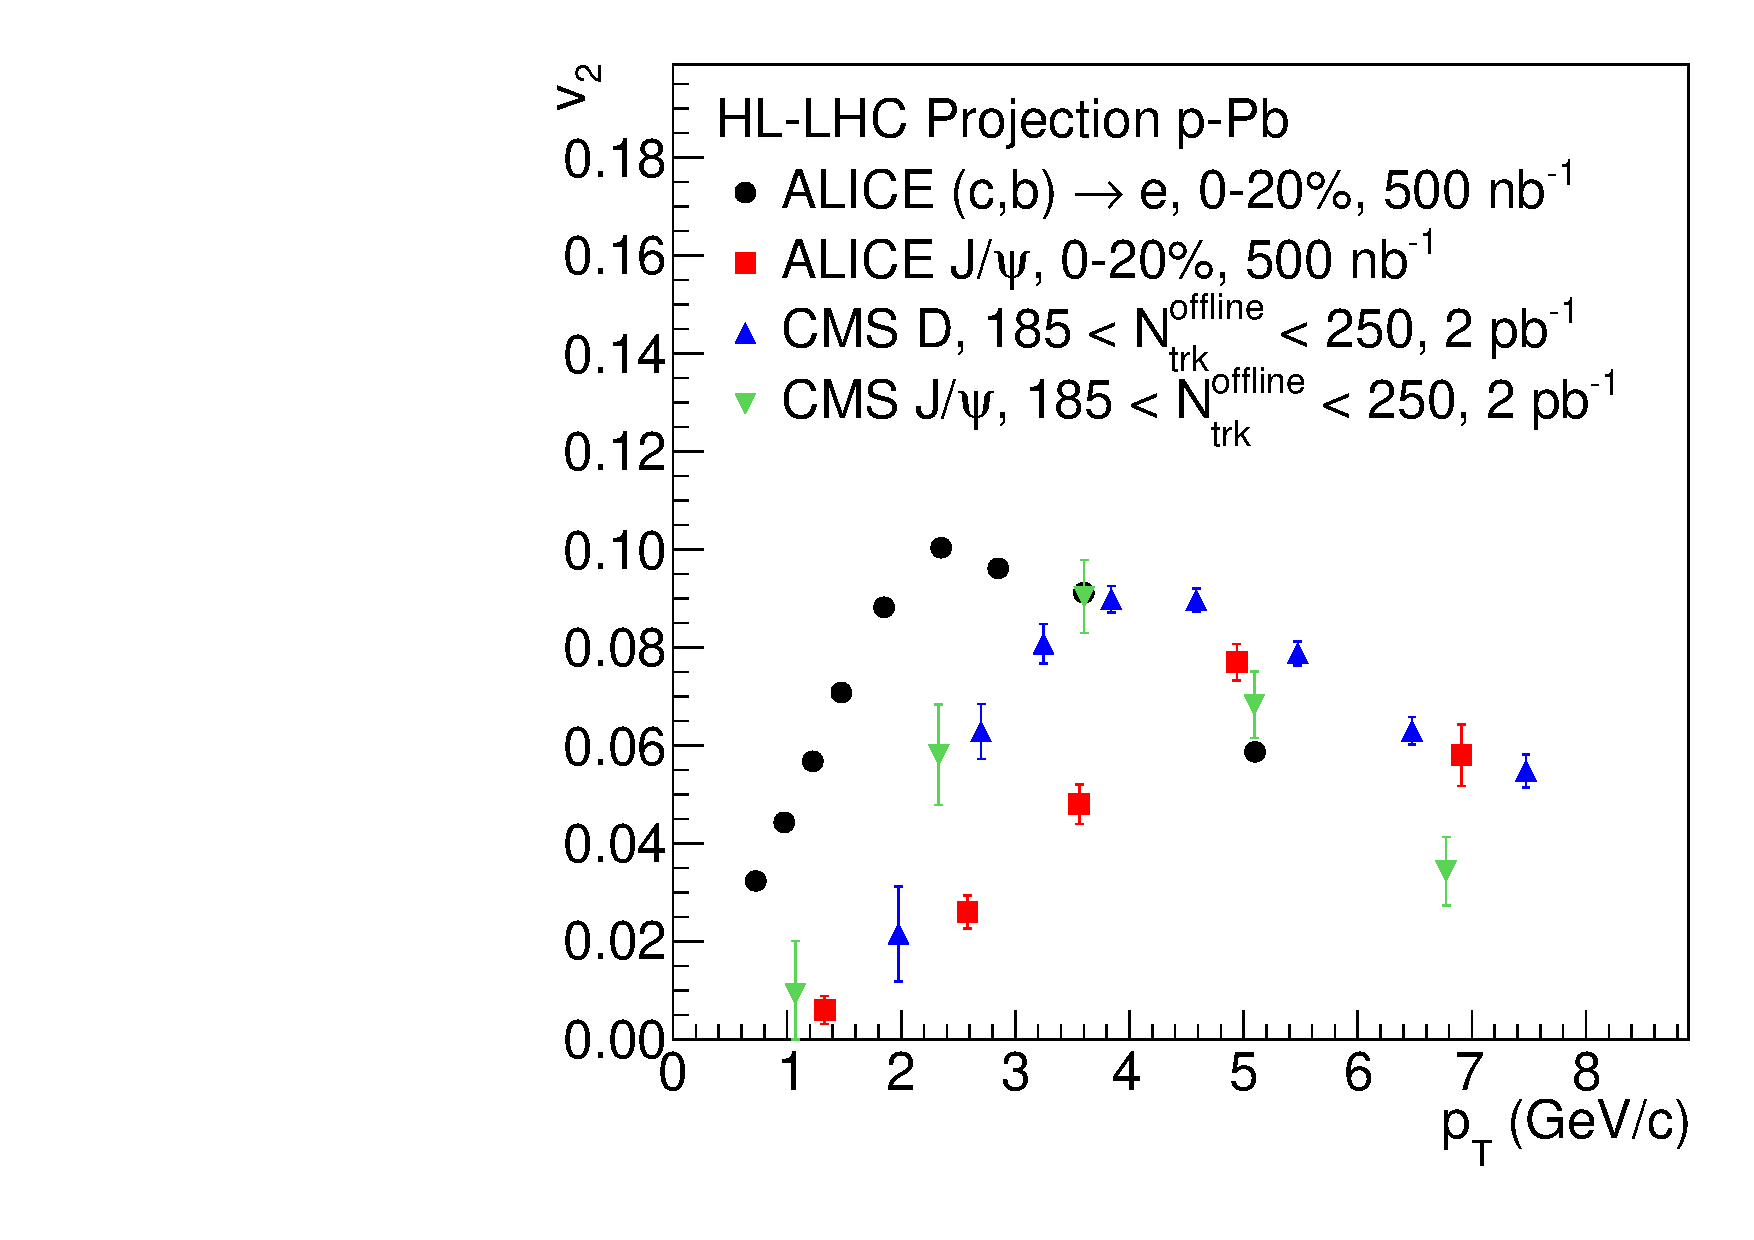
\includegraphics[width=.49\linewidth]{\main/smallsystems/img/v2_ppb.pdf}
\hfill
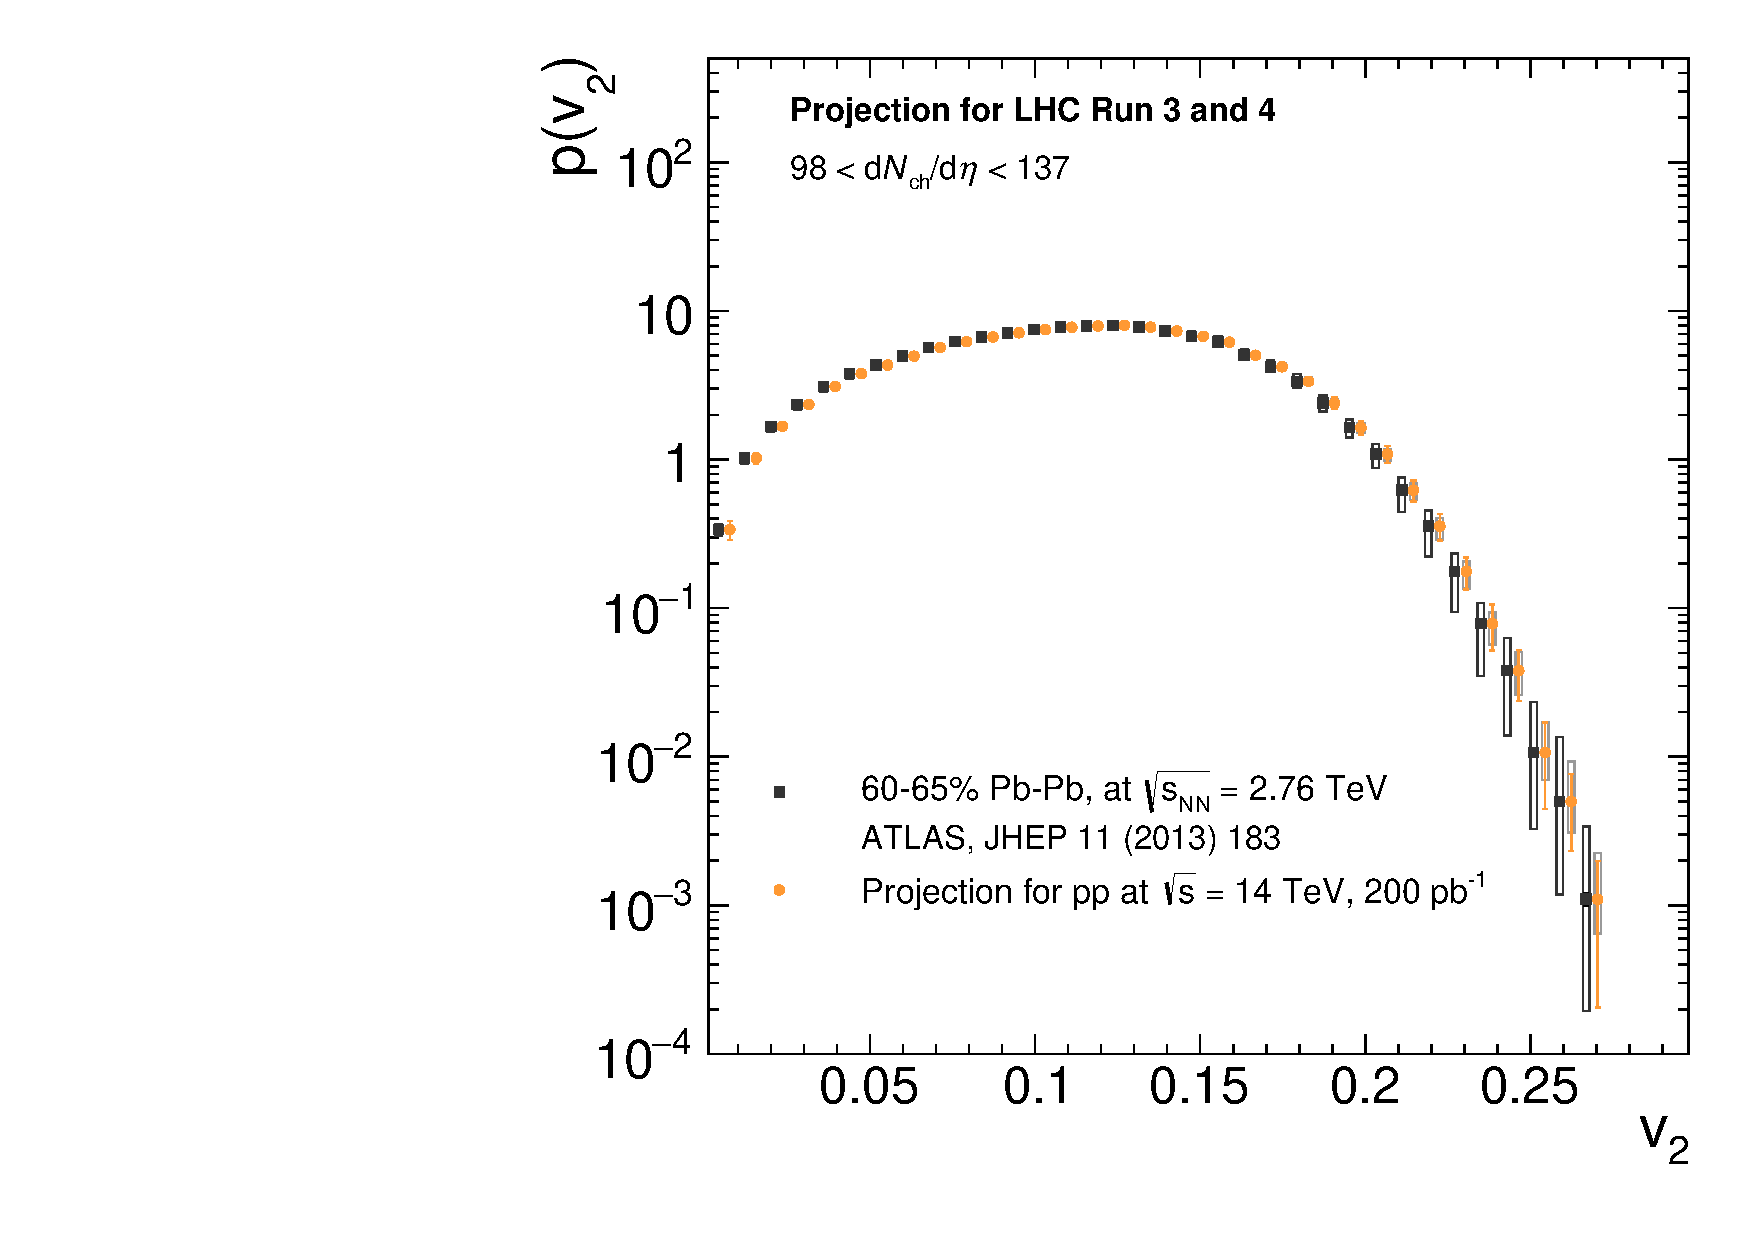
\includegraphics[width=.49\linewidth]{\main/smallsystems/img/ebye_v2_60-65_276TeVppprojection.pdf}
\caption{Left panel: Particle identified $v_{\rm{2}}$ coefficients for \pPb collisions as a function of $\pT$. Two different cases are shown: the ALICE projections are for the 20\% highest-multiplicity collision ($\Lint = \unit[500]{nb^{-1}}$) demonstrating the negligible statistical uncertainties for heavy-flavour decay electrons and $J/\psi$, while the CMS projection is for a bin with $4-5 \meannch$ ($\Lint = \unit[2]{pb^{-1}}$) demonstrating the wide reach in multiplicity achievable for $D$ mesons and $J/\psi$. 
Right panel: Projection of the measurement of the probability distribution of \vtwo in \pp collisions. To illustrate the reach the same signal as in \PbPb~\cite{Aad:2013xma} is assumed although the width of the distribution is most likely smaller in \pp collisions. The projection is for the equivalent \pp multiplicity (circles) as in 60--65\% centrality in \PbPb collisions (squares).}
\label{fig:smallsystems_corr_pid_pvn}
\end{figure}

The correlations of flow harmonics between different orders, called symmetric cumulants, are very sensitive to the initial state and the hydrodynamic evolution. In \PbPb collisions these are, for instance, used to constrain the shear viscosity over entropy ratio $\eta/s$. In addition, they challenge the description of the observed phenomena within initial-state saturation models.
Their measurement in small systems can provide important insight in the validity of the hydrodynamic description of the observed phenomena. Here, symmetric cumulants probe in particular the proton substructure~\cite{Albacete:2017ajt} which is needed to provide a solid description of the initial state, a necessary ingredient for the hydrodynamic description.
The present uncertainties of such measurement in small systems are too large for a definitive conclusion, in particular in \pp collisions, due to the dominance of non-flow like jets and resonance decays. Figure~\ref{fig:smallsystems_corr_symmetriccumulants} shows the performance projection of ${\rm SC}(2,3) = \langle v_2^2 v_3^2 \rangle - \langle v_2^2 \rangle \langle v_3^2 \rangle$ for HL-LHC for \pp and \pPb collisions. The uncertainties of the measurement without subevents becomes practically invisible, however, those stay dominated by non-flow effects. A measurement requiring two, three and even four subevents becomes possible with uncertainties of the order of a few times $10^{-7}$ depending on multiplicity. Such results can give a definitive answer if a similar hydrodynamic footprint is observed in small and large systems.

Figure~\ref{fig:smallsystems_corr_eta4} illustrates the reduction of the statistical uncertainty due to the larger tracker acceptance in Run~4 for ATLAS and CMS. For this 4-particle correlator a reduction of the uncertainties of about 2.5 is expected, and therefore even the measurement of a 1\% $v_3\{4\}$ signal comes into reach. The influence of the acceptance increase on 6- and 8-particle will be larger, factor 4 and 6.5, respectively. Similarly, the uncertainties on the SC measurement reduce significantly at larger \pT.

Figure~\ref{fig:smallsystems_corr_pid_pvn} (left panel) illustrates the reach which can be obtained for the $\vtwo$ measurement of heavy-flavoured objects in \pPb collisions. Shown are projections for heavy-flavour electrons and inclusive $J/\psi$ by ALICE as well as for prompt $D$ and $J/\psi$ by CMS. Minor uncertainties are expected for this observable with the potential to demonstrate for the first time with significance the final-state interaction of charm and beauty in a small collision system.

The \vn fluctuates on an event-by-event basis as no two nuclei have identical parton distribution. The probability density distribution of \vn, ${\rm p}(\vn)$ is closely related to event-by-event fluctuations of the eccentricities, ${\rm p}(\varepsilon_{\rm{n}})$ as $\vtwo \propto k_{\rm{2}\epsilon_{\rm{2}}}$. Therefore its measurement provides crucial information about the initial conditions and the final-state dynamics of the medium. To characterise the initial-state spatial anisotropy these measurements are fitted with Bessel-Gaussian and elliptic power functions. The measurements of probability density distributions for \vtwo at \PbPb collisions are described well by the Bessel-Gaussian function at central collisions and less in peripheral collisions~\cite{Aad:2013xma,Sirunyan:2017fts,Acharya:2018lmh}. This deviation from the Bessel-Gaussian function is expected in peripheral collisions as $k_{\rm{2}}$ increases slightly at large $\epsilon_{\rm{2}}$ values~\cite{Jia:2014jca}. Measurements are well described by the elliptic power functions in all centrality intervals of \PbPb collisions~\cite{Sirunyan:2017fts}. These measurement have not yet been attempted in small systems due to the insufficient available statistics. Figure~\ref{fig:smallsystems_corr_pid_pvn} (right panel) presents a projection for the measurement of ${\rm p}(\vn)$ in \pp collisions. This extrapolation is based on the ${\rm p}(\vtwo)$ measurement in 60--65\% centrality \PbPb collisions at $\sqrtsNN = \unit[2.76]{\UTeV}$~\cite{Aad:2013xma}. The same signal is assumed although the width of the distribution is most likely smaller in \pp collisions. Such a measurement would constitute the first measurement of ${\rm p}(\vn)$ in \pp collisions, and can shed important light on the nature of the observed \vtwo coefficients.


\subsection{Strangeness enhancement}
\label{sect:smallsystems_strangeness}

The unexpected increase of the strange-particle yield normalized by the pion yield as a function of $\nch$ is one of the key observations in small systems. In \pp collisions these ratios are measured up to $\dNdeta \approx 17$ with some overlap with \pPb collisions. The most peripheral \PbPb collisions measured have a $\dNdeta \approx 96$, nearly 6 times larger. Figure~\ref{fig:smallsystems_strangeness_omega_pi} presents the expected reach of the $\Omega/\pi$ ratio in \pp collisions which will bridge the present gap between \pp and \PbPb collisions. In particular, if the measured increasing trend would continue, the $\Omega/\pi$ ratio would grow larger than in peripheral \PbPb collisions. 
Assuming that strangeness enhancement scales with the energy density of the system, Fig.~\ref{fig:small_systems_energy_density} suggests that it should indeed be possible to see that the high-multiplicity \pp results exceed the low multiplicity \PbPb results (crossover). Whether the signature will be as striking as the projection in Fig.~\ref{fig:smallsystems_strangeness_omega_pi}, depends on the details of the assumed scaling law. At this point simulations are not precise enough to provide quantitative predictions of such a crossover, and HL-LHC experimental results on strangeness enhancement will as such be driving the theoretical development.
The scenario with a clear crossover will be immediately distinguishable from a scenario where the $\Omega/\pi$ ratio flattens, and connects smoothly with the \PbPb result. Such a result will in itself also be groundbreaking, as it will indicate that the thermal limit reached in \PbPb collisions will already be realized in high multiplicity \pp collision.

\begin{figure}[t]
\centering
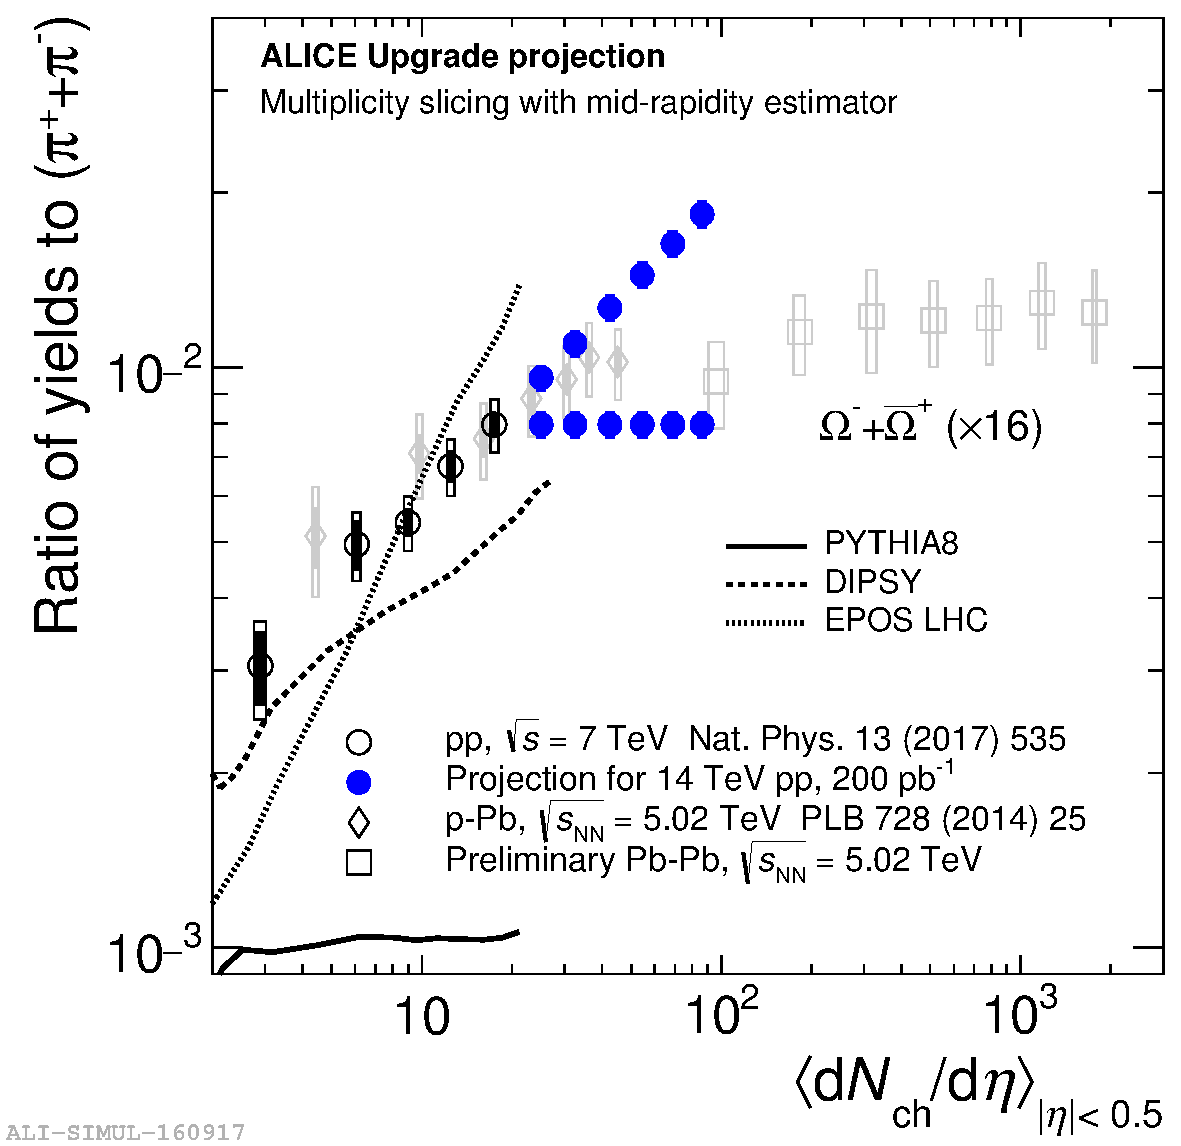
\includegraphics[width=0.49\linewidth]{\main/smallsystems/img/strangeness_omegapi.pdf}

\caption{$\Omega/\pi$ ratio as a function of $\dNdeta$ for \pp, \pPb, and \PbPb collisions. The existing data (from Ref.~\cite{ALICE:2017jyt}) is shown in open black symbols (\pp), grey diamonds (\pPb) and grey squares (\PbPb), while the extrapolation for \pp collision is shown in blue filled circles. Two scenarios are shown: a) assuming that the ratio continues increasing following the measured trend, and b) assuming that the value stays the same as at the largest measured $\dNdeta$.}
\label{fig:smallsystems_strangeness_omega_pi}
\end{figure}

\subsection{Energy loss}
\label{sect:smallsystems_energyloss}

\begin{figure}[t]
\centering
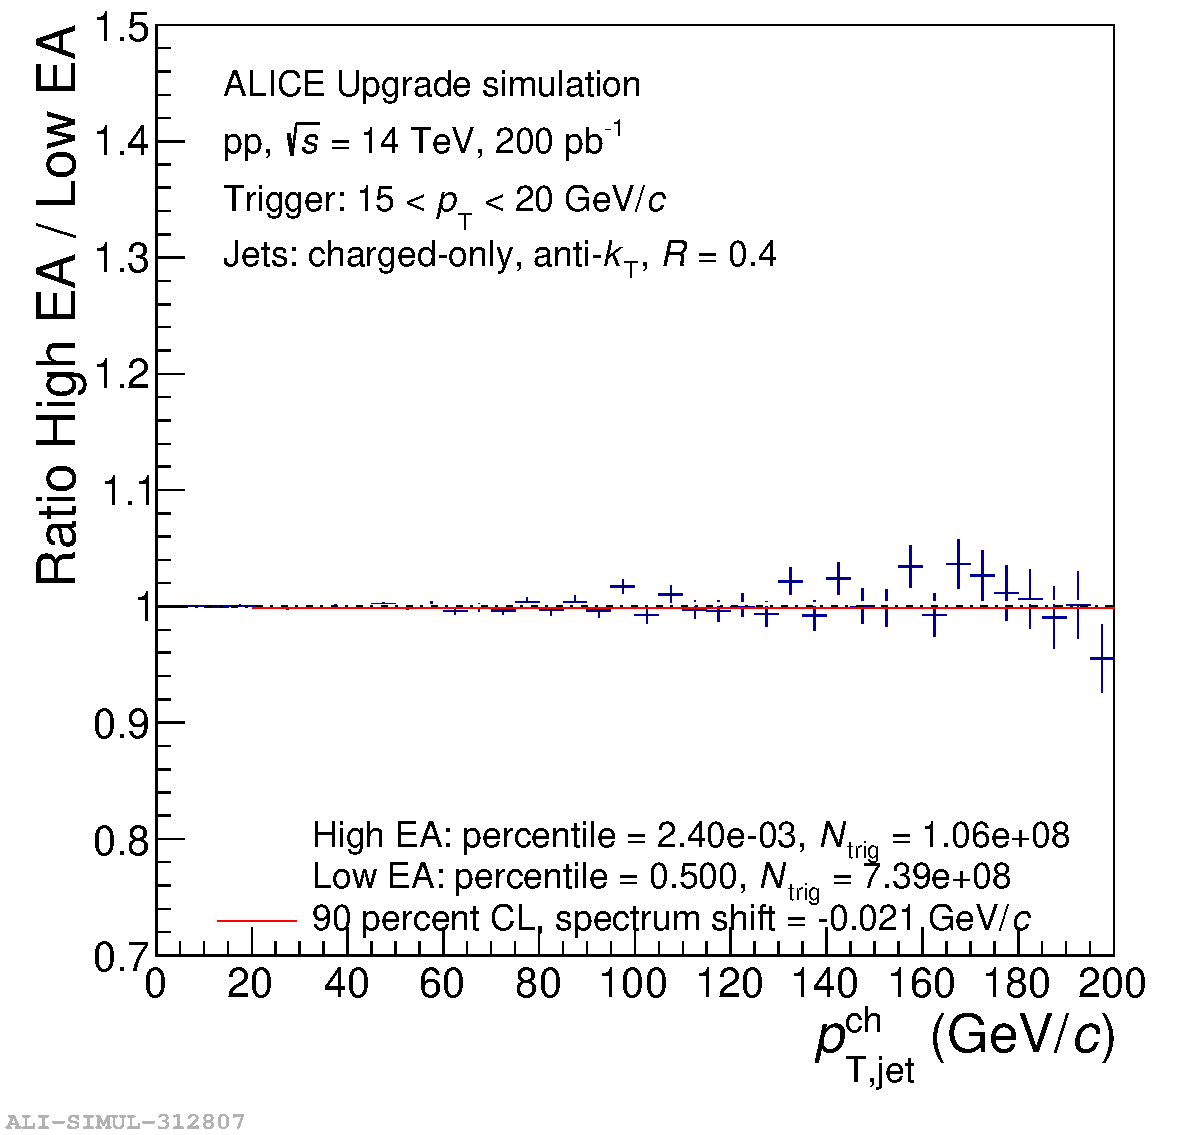
\includegraphics[width=0.49\linewidth]{\main/smallsystems/img/hjet_pp.pdf}
\hfill
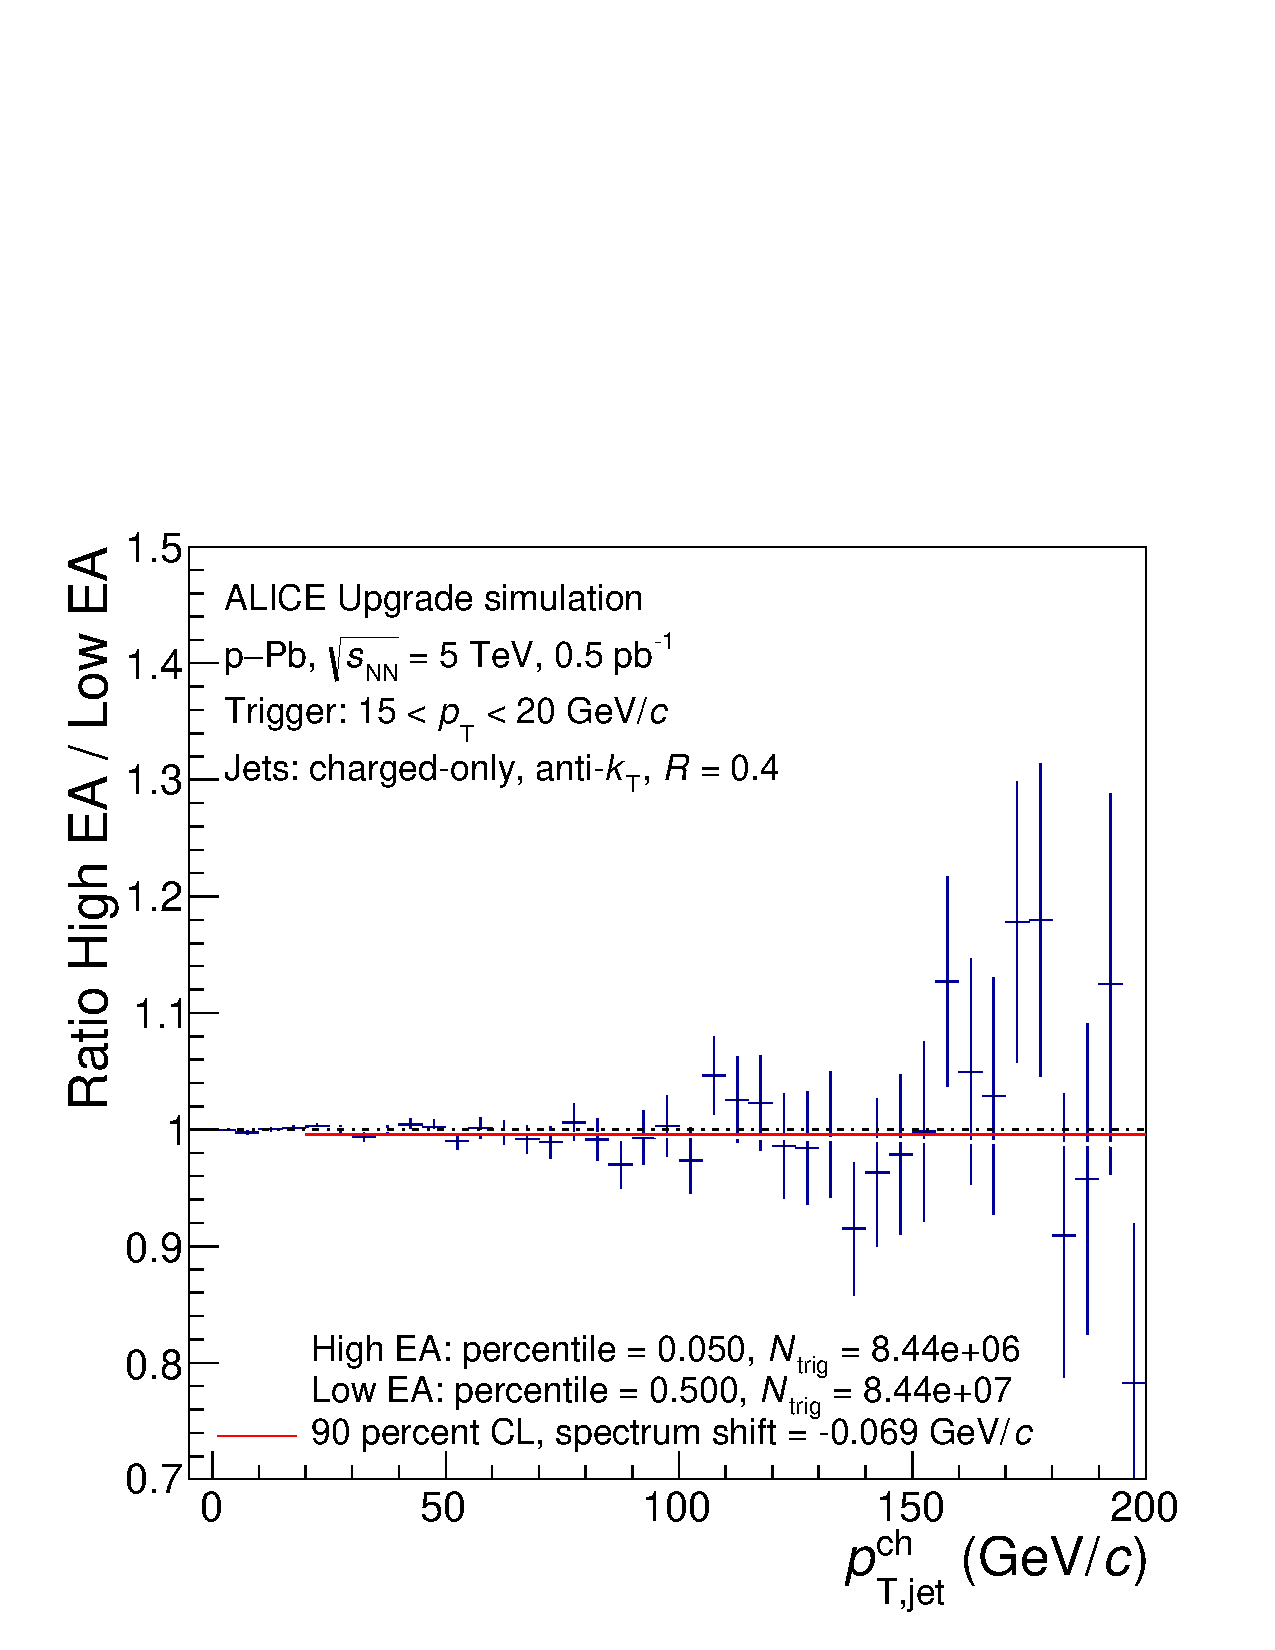
\includegraphics[width=0.49\linewidth]{\main/smallsystems/img/hjet_ppb.pdf}
\caption{Modification of jet recoil yields extracted from semi-inclusive hadron--jet correlations for \pp collisions (left) and \pPb collisions (right) within the ALICE acceptance. Shown is the ratio  of high event-activity (EA) and low-EA recoil spectra as a function of $p_{\rm T,jet}^{\rm ch}$, with high-EA corresponding to 5--7~$\meannch$ in \pp collisions (left panel), and the 0--5\% bin for \pPb collisions (right panel). Since no EA-dependent shift is imposed, the parent distribution of the ratio has the value of unity at all \pT. The red lines show the 90\% CL limit for a possible EA-dependent spectrum shift.}
\label{fig:smallsystems_energyloss_hjet}
\end{figure}

\begin{figure}[t]
\centering
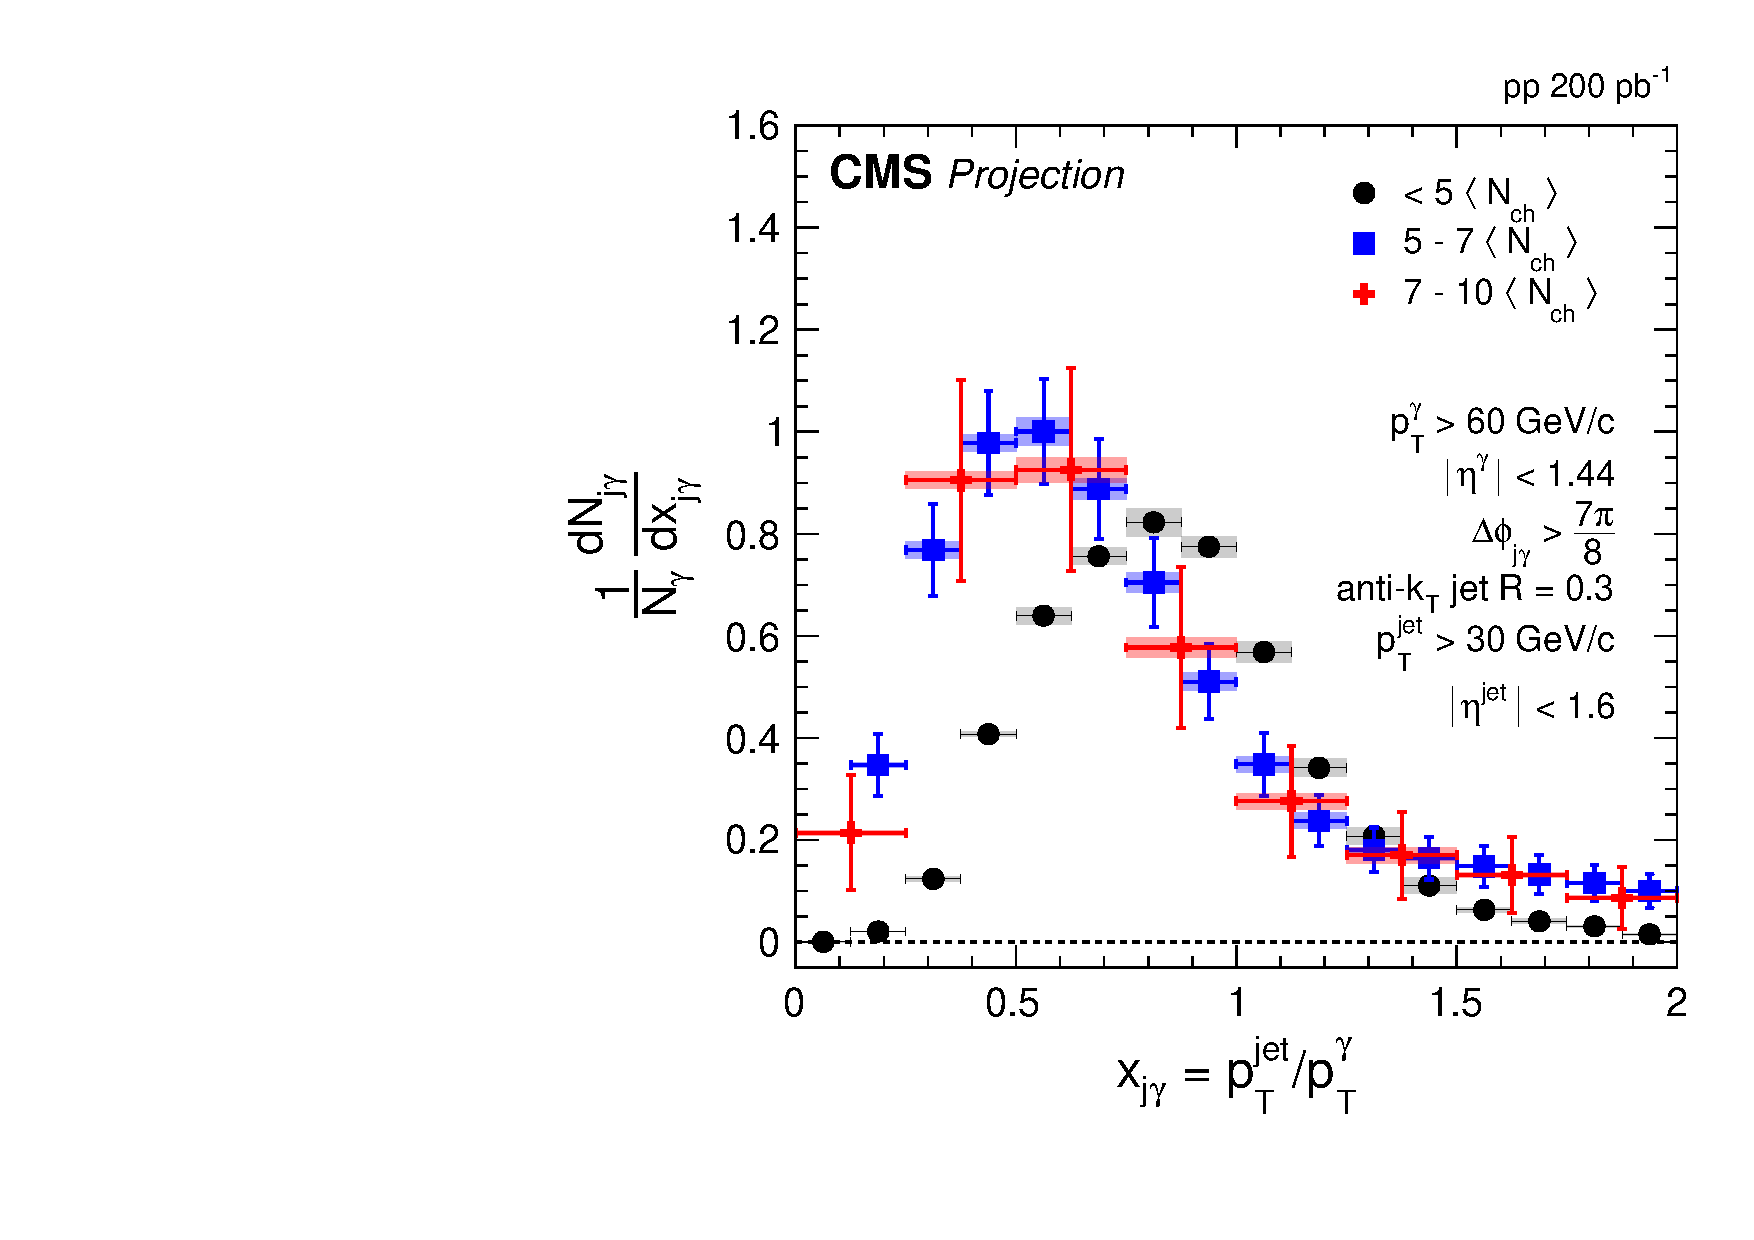
\includegraphics[width=0.49\linewidth]{\main/smallsystems/img/xjg_highmult_projection_rebin.pdf}
\hfill
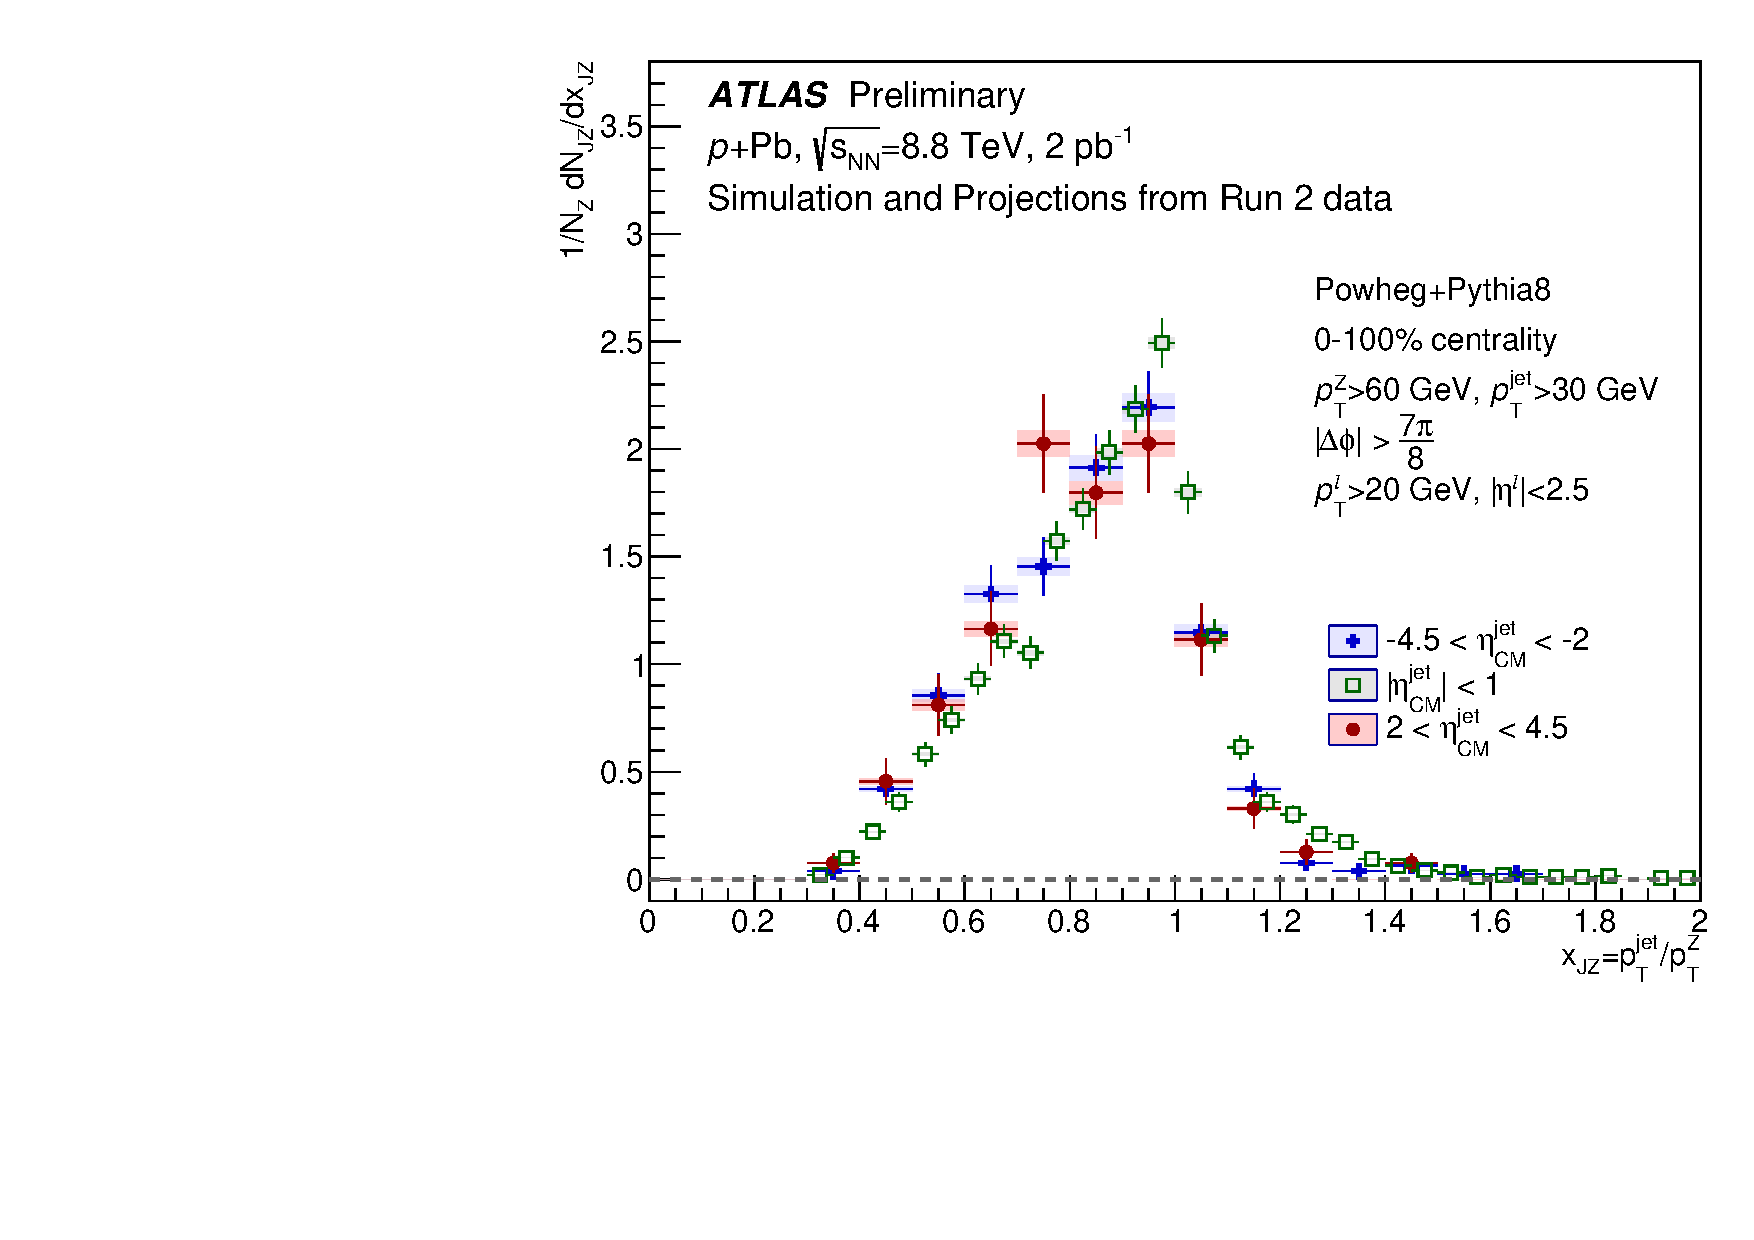
\includegraphics[width=0.49\linewidth]{\main/smallsystems/img/atlas_xj_dist_cm_2bins_forward_flipped.pdf}
\caption{Left panel: CMS projection of the measurement of the jet--$\gamma$ momentum fraction $x_{j\gamma}$ in \pp collisions for selected high-multiplicity bins. A jet with $\pT > \unit[30]{\UGeVc}$ is required to be back-to-back ($\Delta\varphi > 7/8\pi$) with a $\gamma$ with $\pT > \unit[60]{\UGeVc}$. The shape is based on Pythia. Figure from Ref.~\cite{CMS-PAS-FTR-18-025}. Right panel: ATLAS projection of the measurement of the jet--$Z$ momentum fraction $x_{jZ}$ in \pPb collisions in different pseudorapidity intervals. The momentum requirements are also \unit[30]{\UGeVc} for the jet and at least \unit[60]{\UGeVc} for the $Z$, with the same back-to-back requirement ($\Delta\varphi > 7/8\pi$). The projection is based on Powheg + Pythia 8 Monte Carlo samples with the CT10 PDF set. Figure from Ref.~\cite{}. UNDER APPROVAL.}
\label{fig:smallsystems_energyloss_xjg_xjz}
\end{figure}

As discussed in Sect.~\ref{sect:smallsystems_historicoverview}, inclusive high-\pT hadron and jet yields show at present no evidence of medium-induced energy loss in \pPb collisions, and suffer from selection biases if measured in event classes. 
%Furthermore, these typically require a unmodified reference, and can therefore not easily applied to \pp collisions itself. 
Inclusive measurements with the large event set expected at HL-LHC therefore do not help to resolve the question of energy loss in small systems. However, coincidence measurements of jets recoiling against a trigger object are not subject to such biases, and have the potential to identify small energy-loss effects or put stringent upper limits. In this section, projections are given for correlations between high-\pT hadrons and jets, as well as jets and $\gamma$ and $Z$.

Figure~\ref{fig:smallsystems_energyloss_hjet} shows a projection of the measurement of semi-inclusive hadron--jet correlations in LHC Run 3 and 4, for \pp collisions at $\sqrts = \unit[14]{\UTeV}$ and \pPb collisions at $\sqrtsNN = \unit[5.02]{\UTeV}$. The figure shows the ratio of trigger-normalized recoil spectra for events selected on high and low event-activity (EA) classes. 
This projection is based on Pythia simulations for \pp collisions, which gives the expected number of charged-hadron triggers in the interval $15<\ptt<20$~\UGeV\ (scaled by $A$ to model \pPb collisions), and the per-trigger recoil jet spectrum. The measured enhancement in the per-event high-\pT hadron yield for \pp collisions in high-multiplicity collisions~\cite{Acharya:2018orn} has been taken into account.

The projection represents the case where no energy loss occurs for high-EA relative to low-EA collisions, and demonstrates the statistically achievable limit. The 90\% confidence level for a possible EA-dependent spectrum shift due to large-angle energy transport from jet quenching~\cite{Acharya:2017okq} is \unit[70]{\UMeVc} for \pPb (5\% highest EA) and \unit[21]{\UMeVc} for \pp collisions (5--7~$\meannch$). These values are over 100 times smaller than the spectrum shift measured in \PbPb collisions~\cite{Adam:2015doa}. The high statistics of the HL-LHC dataset enables this approach to be applied to yet more stringent EA selections; for 7--10~$\meannch$ (10--12~$\meannch$) the corresponding 90\% CL limit on energy loss is expected to be \unit[69]{\UMeVc} (\unit[590]{\UMeVc}).

Projections for the correlation of jets and $\gamma$ as well as jets and $Z$ are presented in Fig.~\ref{fig:smallsystems_energyloss_xjg_xjz} for \pp and \pPb collisions. Shown are distribution of the momentum fraction $x_{jX} = \pT^{\rm jet}/\pT^X$ where $X$ is the $\gamma$ or $Z$. Given that the $\gamma$ and $Z$ can be considered unmodified by final-state interactions, a potential energy loss acting on the jet would directly alter the $x_{jX}$ distribution. For \pp collisions, the left panel of Fig.~\ref{fig:smallsystems_energyloss_xjg_xjz} presents the distribution for different classes in multiplicity based on Pythia, demonstrating the reach. 
It is, however, also seen that the distribution shifts significantly, without final-state interactions, but purely due to the presence of an underlying event. As this shift closely mimics the signature on jet quenching, while at the same time being highly sensitive to the underlying event, the importance of solid understanding of this type of background should be underlined.
The right panel of Fig.~\ref{fig:smallsystems_energyloss_xjg_xjz} presents the projection for \pPb collisions for MB collisions but in different pseudorapidity intervals sensitive to potential differences in the p and Pb hemisphere.

\subsection{Thermal Radiation}
\label{sect:smallsystems_thermalradiation}

\begin{figure}[t]
\centering
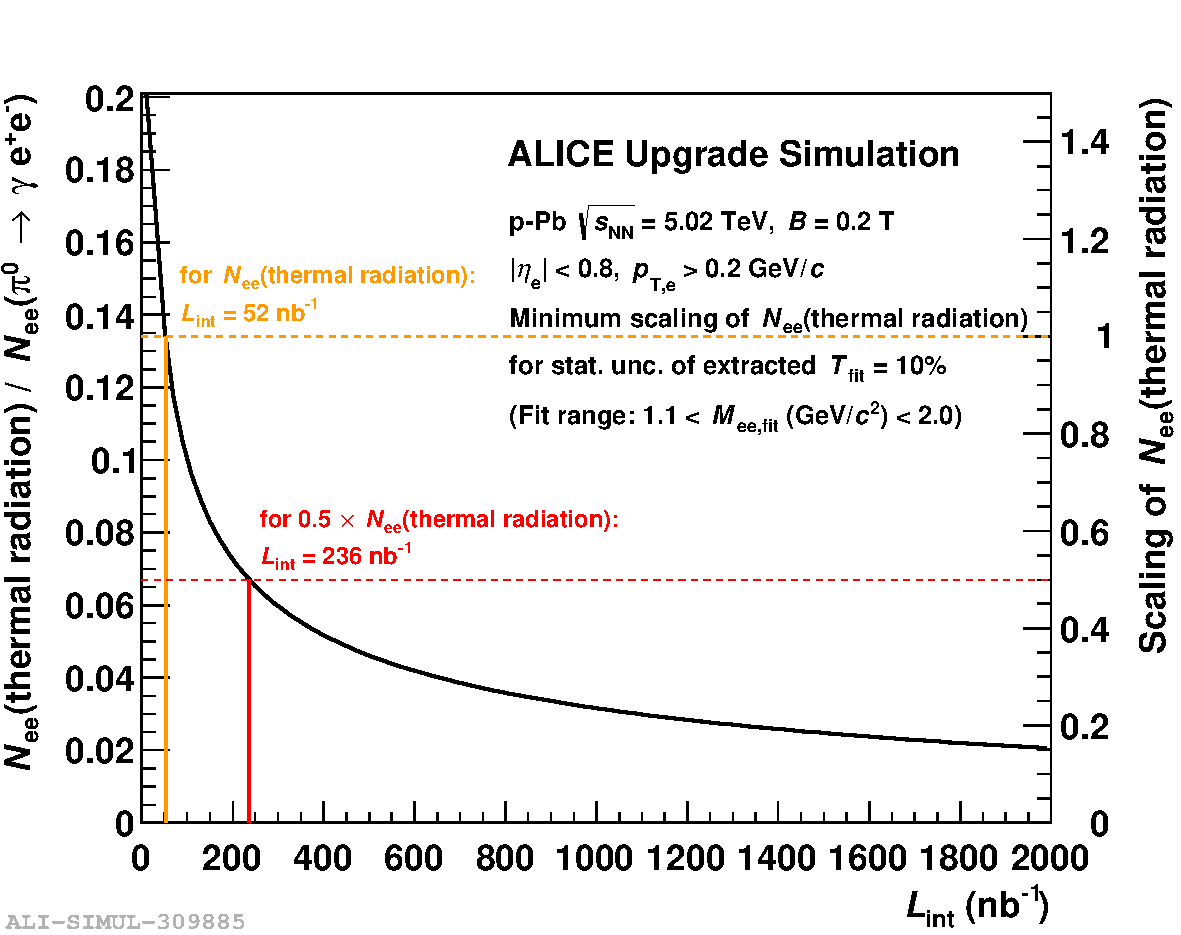
\includegraphics[width=0.6\linewidth]{\main/smallsystems/img/2018-10-26-finalPlotsTemperatureComparison_pPb_FastSim_FitBG_noDCAcut_fitResults_study010_33_38}
\caption{Projection of the measurement of the medium temperature extracted from thermal dileptons in \pPb collisions. As the expected signal is uncertain, the figure presents the required integrated luminosity relative to the prediction based on Ref.~\cite{Rapp:2011is} denoted by $N_{\rm ee}$(thermal radiation). It is expressed as the minimum thermal photon $N_{\rm ee}$(thermal radiation) to $\pi^0$ ratio (left axis) and scaling of $N_{\rm ee}$(thermal radiation) (right axis) for achieving a 10\% statistical uncertainty on the extracted temperature.}
\label{fig:smallsystems_thermal_radition}
\end{figure}

The measurement of thermal radiation in \pPb collisions can be considered as a smoking gun for the formation of a system with an energy scale above the phase transition temperature, see Chapter~\ref{chapter:electromagnetic_radiation}. In order to estimate the sensitivity to the thermal radiation in \pPb collisions, a similar strategy as in Sec.~\ref{sec:thermalradiation:dileptons} was used.
The combinatorial background was scaled from \PbPb collisions to the expected number of pairs in \pPb collisions. The pair efficiency (including the efficiency for rejecting \Pepem pairs from semileptonic charm decays) is assumed to be the same as in \PbPb collisions.
Subsequently, the temperature of the QGP is extracted in the same way as in Sec.~\ref{sec:thermalradiation:dileptons}. The minimum thermal photon to $\pi^{0}$ (both decaying into \Pepem) ratio that is needed for a fit to the invariant mass spectrum with a statistical uncertainty $\sigma_{\rm T,stat} = 10\%$ as a function of \Lint\ up to \unit[2000]{nb$^{-1}$} is shown in Fig.~\ref{fig:smallsystems_thermal_radition}. If the considered prediction is accurate, an integrated luminosity of about $\unit[50]{nb^{-1}}$ is sufficient for the measurement. In case the signal is 50\% smaller about 4--5 times the statistics is needed.

\begin{figure}[t]
\centering
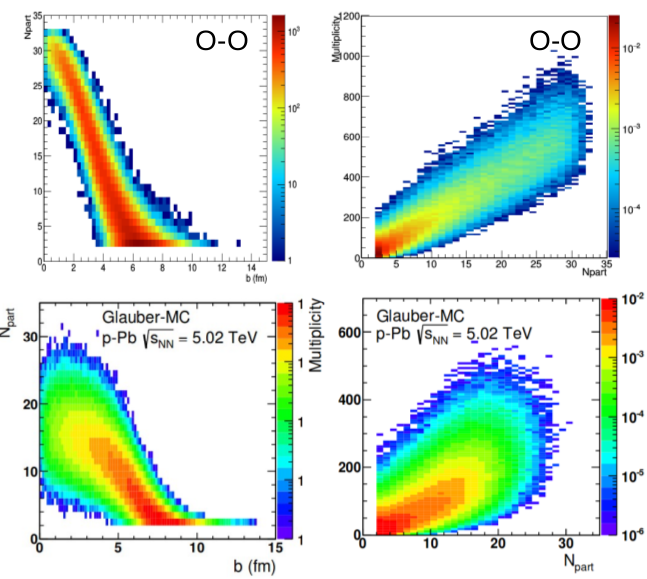
\includegraphics[width=0.8\linewidth]{\main/smallsystems/img/oo-geom}
\caption{Glauber MC calculations are presented for for \pPb (top panels) and \OO collisions (bottom panels). Shown are \Npart as a function of impact parameter (left panels) and forward multiplicity as a function of \Npart (right panels).}
\label{fig:smallsystems_oo_glauber}
\end{figure}


\begin{figure}[t]
\centering
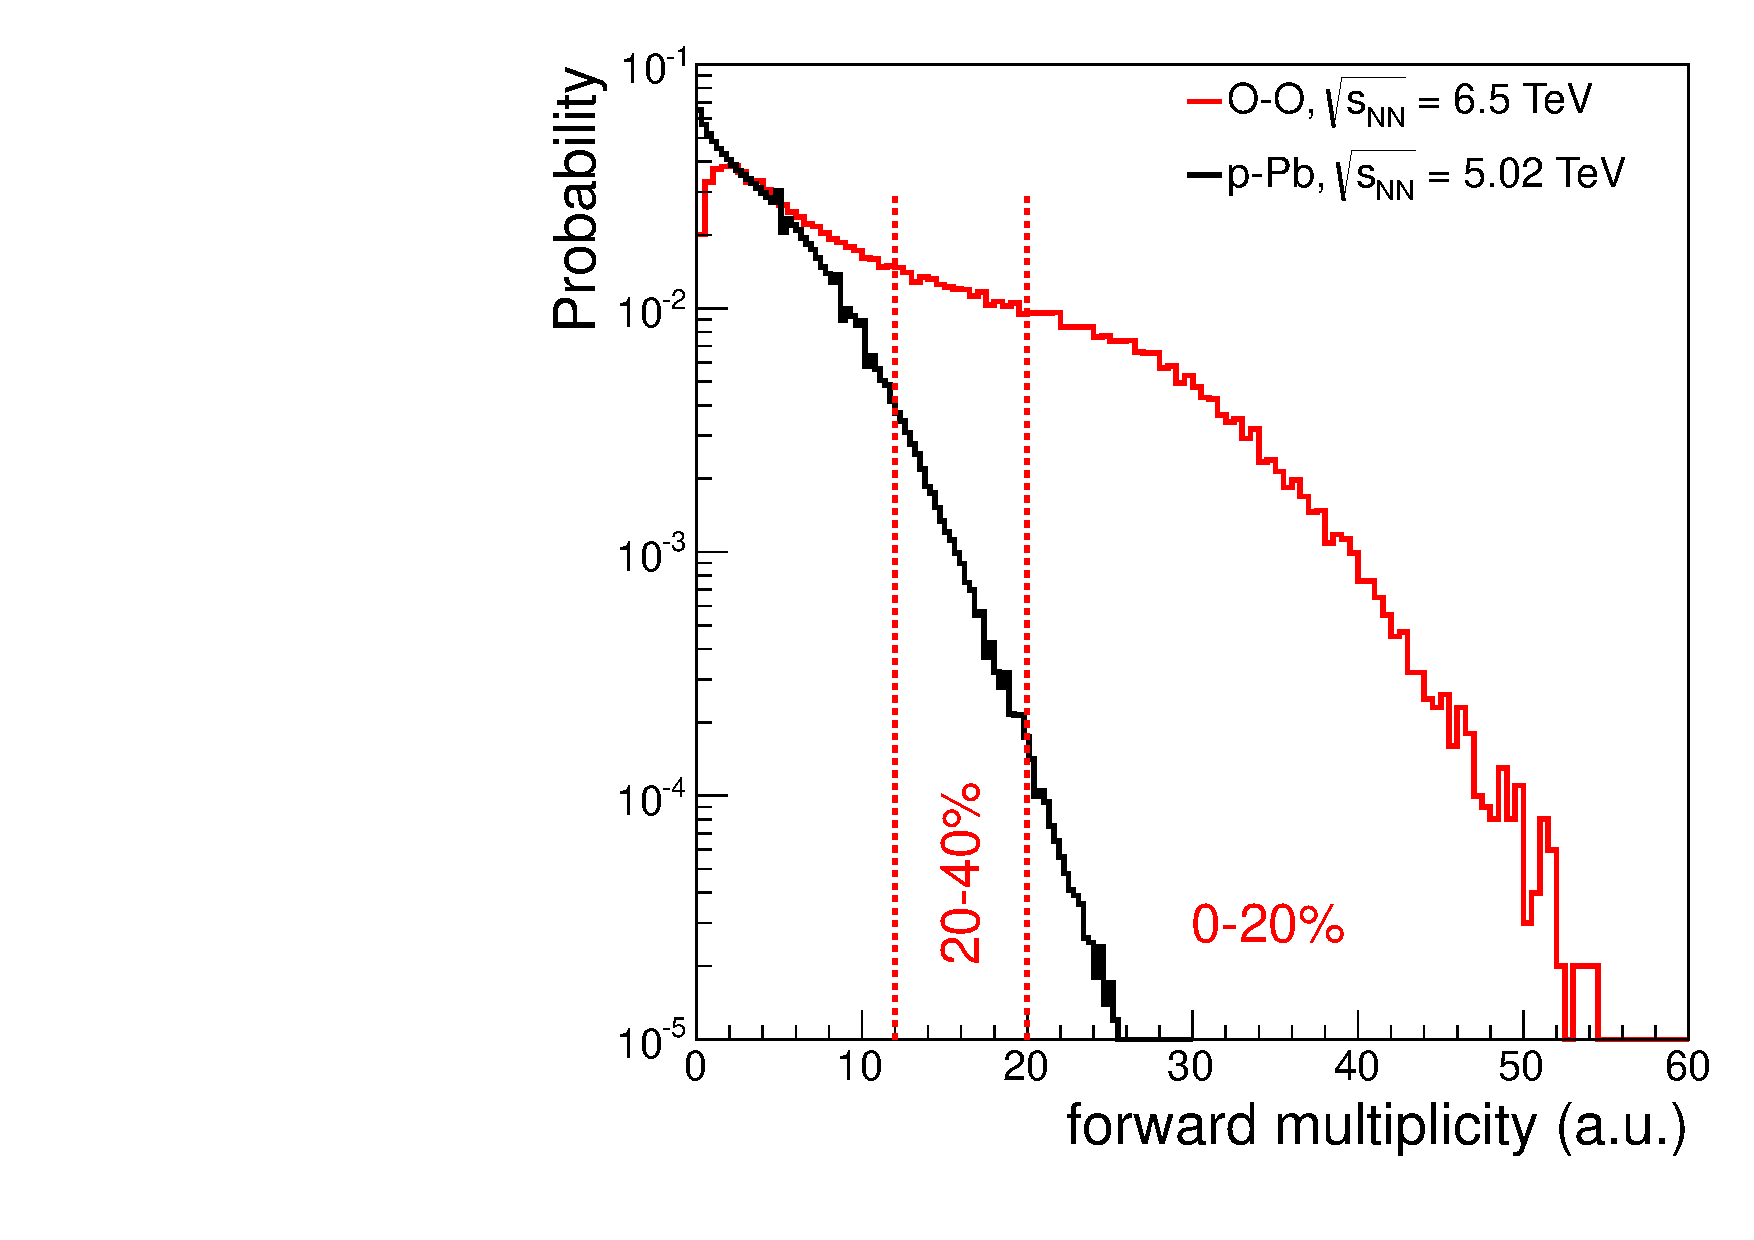
\includegraphics[width=0.5\linewidth]{\main/smallsystems/img/oo-cent}
\caption{Estimated multiplicity distributions in the forward region in \OO and \pPb collisions. The event classes of highest multiplicity in \OO collisions are indicated with 0--20\% and 20--40\%.
The \OO studies have been been performed for the 2018 beam configurations at $\sqrtsNN = \unit[6.5]{\UTeV}$, while the Run 3 configuration would yield $\sqrtsNN = \unit[7]{\UTeV}$, with the advantage that a large \pp reference data set already exists from earlier LHC running (2010--11).
}
\label{fig:smallsystems_oo_mult}
\end{figure}

\subsection{Potential of \OO Collisions}
\label{sect:smallsystems_OO}

A promising opportunity to study the emergence of collective phenomena further as well as the presence of possible parton energy loss in small collision systems, are collisions of smaller nuclei. 
In particular, collisions of Oxygen-16 are a very efficient way of investigating the properties of low-multiplicity heavy-ion collisions, which in large \AOnA systems only occurs for peripheral geometries.
The achieved multiplicities in \OO collisions are similar to \pPb collisions with the significant advantage that the collision geometry is much better defined.
This is demonstrated in Fig.~\ref{fig:smallsystems_oo_glauber}, which shows the correlations between number of participants, multiplicities and impact parameter in \OO and \pPb collisions. The correlations between \Npart and impact parameter as well as multiplicity and \Npart is much narrower in \OO collisions as compared to \pPb collisions. Consequently, highest multiplicities in \pPb collisions are only accessible in the tail of the distribution while similar multiplicities are already reached in \OO collisions in the plateau region. This is shown in Fig.~\ref{fig:smallsystems_oo_mult} illustrated by the 20--40\% event class.

Scaling the measured nuclear-modification factor in \PbPb collisions at \unit[5.02]{\UTeV}~\cite{Acharya:2018qsh} at similar multiplicities as for central \OO collisions while roughly accounting for the artificial suppression caused by the multiplicity bias present in such peripheral \PbPb collisions~\cite{Acharya:2018njl}, allows to estimate the expected \RAA in \OO collisions to about 20\%.
Out of this deviation from unity, about half can be attributed to biases due to the multiplicity selection in such small collision systems already in absence of nuclear effects~\cite{Adam:2014qja}. An observable deviations from unity of about 10\% caused by energy loss in the produced medium remains. While this expected suppression may seem small, it should be possible to measure it already with an $\Lint$ of a few $\unit[100]{\mu b^{-1}}$. 
In case such a suppression was absent, the conclusion can be drawn that such small collision systems do not exhibit measurable energy loss, while other collective features are present.
It should be noted that the absence of suppression can most likely not be taken as a proof against the formation of the QGP, as it may be that the fast partons are emerging without seeing the medium (surface effect).

\begin{figure}[t]
\centering
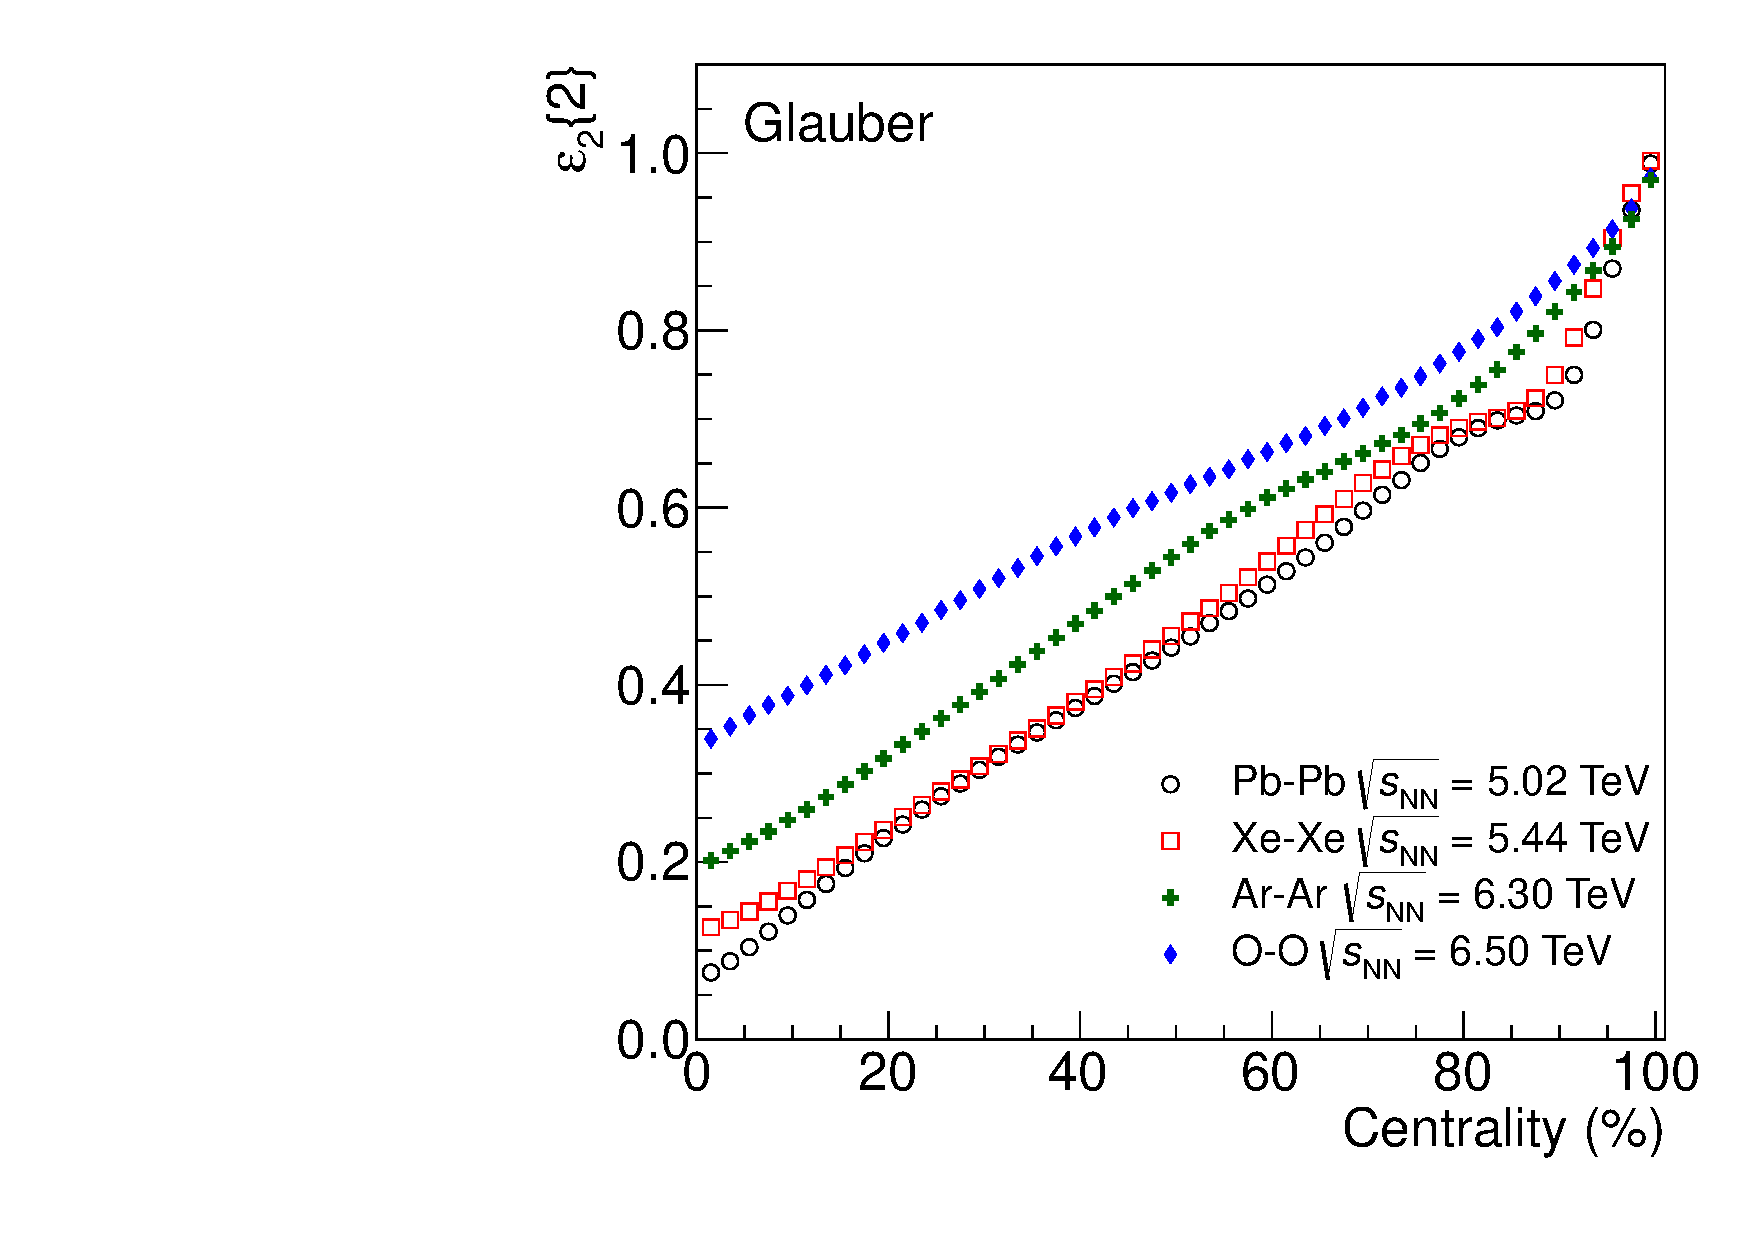
\includegraphics[width=0.48\linewidth]{\main/smallsystems/img/eps2_glauber}
\hfill
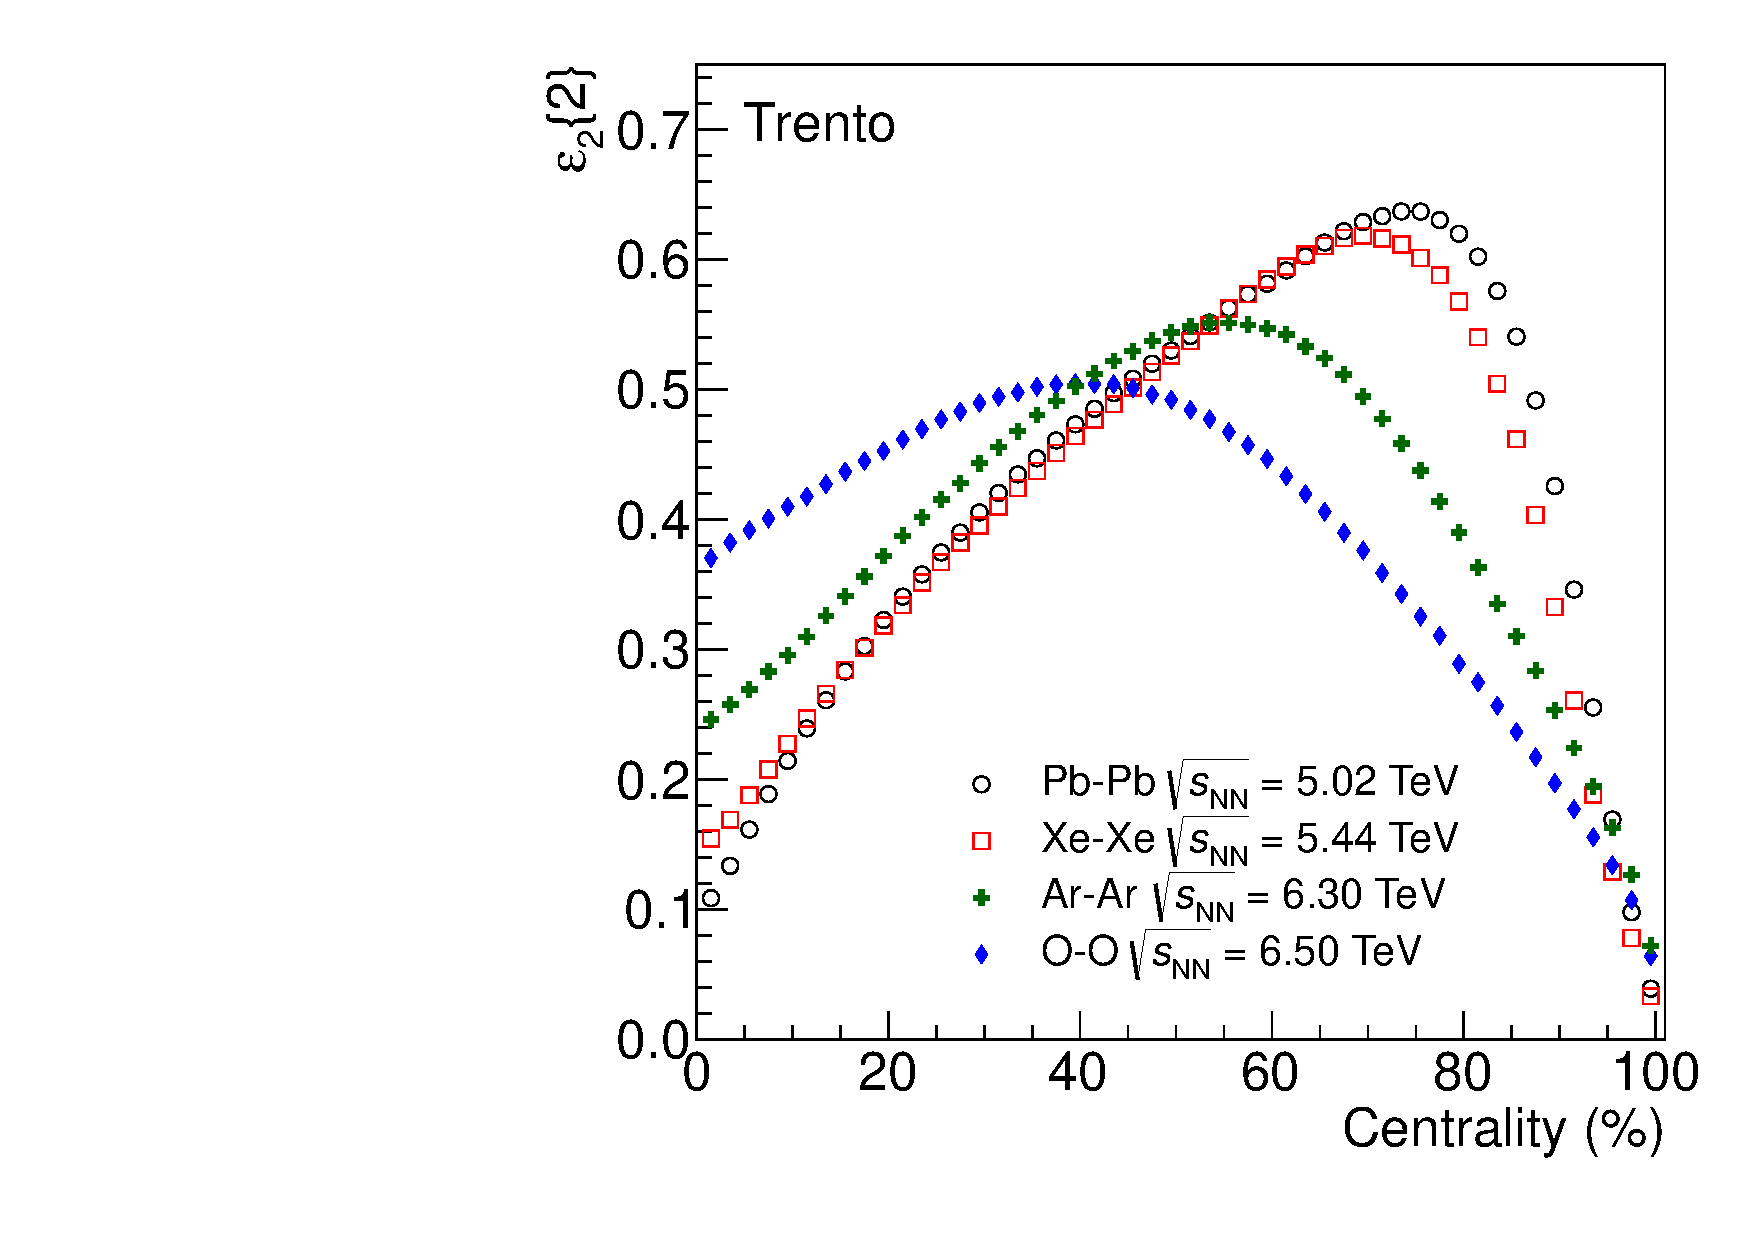
\includegraphics[width=0.48\linewidth]{\main/smallsystems/img/eps2_trento}
\caption{Second-order eccentricity coefficient $\epsilon_2$ as a function of centrality for \OO, \ArAr, \XeXe and \PbPb collisions from MC-Glauber (left panel)~\cite{Miller:2007ri,Loizides:2017ack} and Trento (right panel)~\cite{Moreland:2014oya} initial conditions.}
\label{fig:smallsystems_ecc}
\end{figure}

A strong correlation between initial state geometry (collision eccentricity) and observed flow has been established since RHIC~\cite{Drescher:2007cd}, and pertains at LHC, also in systems as small as \XeXe~\cite{Acharya:2018ihu}. As shown in Fig.~\ref{fig:smallsystems_ecc}, the eccentricity profiles of \XeXe and \PbPb collisions are, however, quite similar, and collision systems exhibiting a different geometry as \OO could therefore provide further insight into the connection between initial-state geometry and multi-particle correlations.

\subsection{Summary}

The discoveries made in recent years in small collision systems have caused a paradigm shift in the field with impact on both, the modelling of heavy-ion collisions as well as the underlying event of elementary \pp collisions. 
Experimental evidence for final-state interactions in small systems, manifested as strangeness enhancement and multi-particle correlations suggests that energy loss should also be present. But up to this point no hint of energy loss in \pp or \pPb collisions has been seen. The increased luminosity will allow both for precision studies of the established signatures of small system collectivity, and to either establish evidence or place exclusion limits on the latter.

Significant progress is expected in the study of small collision systems at HL-LHC. This chapter has presented a set of performance studies ranging from largely non-flow suppressed high-order correlations, over measurement of strange-particle yields and thermal radiation, to energy-loss signals. Together with expected progress on the theoretical understanding, the community can look forward to a deepened understanding of non-perturbative QCD and a universal description of small to large collision systems in the next decade.

\end{document}
